\chapter	{Compton camera application for ion beam therapy monitoring}

\vfill

\minitoc

\newpage


\section{Introduction}\label{section::Intro}
Ion beam therapy is a cancer treatment technique which is rapidly gaining importance in the global tumor therapy panorama. In addition to the already operational 70 clinical facilities, with more than 175000 patients already treated by the end of 2017, several new centers have been designed and approved for construction worldwide~\cite{PTCOG_stats}. The favorable feature of this treatment technique is connected to the peculiar energy deposition profile of charged particles as a function of depth in matter. As first observed by Bragg~\cite{Bragg_main}, the depth-dose profile of charged particles shows a maximum close to the end of their range in matter; in addition to this, a strong enhancement of the relative biological effectiveness (RBE) is observed for ions heavier than protons in the region of the Bragg peak~\cite{RBE_Elsasser, RBE_Weyrather}, which further enhances the 
dose ratio between target and healthy tissues.

The maximum of the dose is deposited in the Bragg peak region in the patient and must be tuned to cover the target volume (defined via CT scan) and, at the same time, spare the surrounding healthy tissues. Treatment planning and delivery uncertainties limit the tumour targeting capabilities, like uncertainties in the material composition determination, CT units conversion to ion stopping power, patient mis-positioning, organ motion or morphological changes between treatment fractions. These uncertainties force the clinicians to fix relatively large safety margins around the planned treatment volume, up to 3.5\% + 3 mm~\cite{Paganetti:2012aa}. Ion-range verification is one of the conditions required for a broader usage of ion beam therapy and for its further development. With the goal of fully exploiting the ion beam therapy dosimetric potential, the monitoring should be in real-time and ideally in 3 dimensions, in order to detect important deviations between the planned and delivered dose to the target volume or to surrounding organs, in particular in case of proximity to organs-at-risk~(OAR). This capability would allow for a reduction of the above mentioned safety margins and for a better tumor targeting; in addition to this, it could permit the use of new irradiation fields with OAR downstream with respect to the tumor position~\cite{Knopf:2013aa}.   

Several range verification techniques have been considered worldwide for twenty years. Most of them rely on the detection of secondary radiation generated during the slowing down process of incident ions, in particular during nuclear reactions. Among theses secondary radiations, positron emitters have been deeply studied in order to exploit positron emission tomography (PET) machines for treatment monitoring. The only available and functional range monitoring system in a clinical center is based on this technique~\cite{ENGHARDT2004}, which is anyway affected by physical and technical limitations\cite{PARODI2016}.

%PET techniques are based on the detection of the two back-to-back 511~keV photons produced by the annihilation of positrons (created by the emitter fragments of nuclear reactions) with patient electrons, resulting in a delayed radiation which should be detected with time coincidences, allowing for an intrinsic background reduction. Nevertheless, the monitoring with positron emitters secondary signal must deal with a limited count rate compared to medical imaging PET, with the lifetime of emitters providing a delayed information that implies the signal integration over a whole treatment fraction (not a single spot or group of spots), with physiological washout effects depending on to the emitters lifetime.
%
%Even if the only available and functional range monitoring system in a clinical center is based on this technique~\cite{ENGHARDT2004}, several clinical experience with commercial or adapted PET system already shown intrinsic limitations mainly connected to the ring geometry (not directly applicable to the treatment monitoring due to the presence of the beam) or in general to geometrical constraints limiting the field of view and the resulting system global efficiency and spatial accuracy (the limited detection angle generates artifacts in the final image)~\cite{PARODI2016}. The research is ongoing and new results are expected for the next years thanks to the introductions of new systems with adapted geometries, to the improvements in acquisition and reconstruction techniques and to the clinical introduction of time-of-flight systems, intrinsically able to improve the detector spatial resolution via interaction time information, and depth-of-interaction reconstruction, which will allow for a more precise spatial reconstruction for reduced angular artifacts effects.

In addition to positron annihilation products, the relaxation of excited nuclei also produces secondary photons in a wide energy range, between some hundreds of keV till about 8-10~MeV. After the first idea proposal published in 2003~\cite{PG_first}, these secondary products of particle treatment have been deeply investigated and the correlation of this gamma radiation to the ion depth-dose profile has been confirmed by several research groups, starting from~\cite{Min_PG} for protons and~\cite{Testa_PG} for carbon ions. The so-called prompt gamma-rays (PG) have the advantage to be emitted almost instantaneously after the beam interaction in the tissue, making them more adapted than PET 511~keV gammas for real-time monitoring. Moreover, as shown in~\cite{Robert2013}, the emission rate is compatible to the one of the annihilation gammas for both protons and carbon beams. Consequently, different techniques have been proposed to exploit this signal for treatment monitoring purpose, with the related detection systems. Some methods are based on PG timing~\cite{Golnik:2014aa, Krimmer_PGPI} or energy~\cite{Verburg:2014aa} information and rely on non-collimated systems; more complex detection apparatus can achieve an actual PG imaging, by exploiting mechanical or electronic collimation (i.e.~with collimated gamma camera or Compton camera, respectively) for the photon selection (see e.g.~\cite{Min_PG, Bom_collimated, Priegnitz:2015aa, Smeets:2012aa, Roellinghoff_2014, Frandes_2010, LLOSA2012105, KORMOLL2011114, MCCLESKEY2015163, Matsuoka:2014qna, Peterson:2010aa, Solevi:2016aa, ALDAWOOD2017190}). For a review on PG monitoring, see~\cite{krimmer:hal-01585334}.

Originally designed for astrophysics applications, the potential of Compton cameras for medical imaging has been soon recognized~\cite{TODD:1974aa} and then directly translated to the ion beam therapy monitoring domain. Such a gamma detection system is generally  composed of two sections: a scatterer and an absorber. The scatterer is dedicated to the gamma Compton scattering, and should be designed to optimize the Compton scattering probability in the prompt gamma energy range, while reducing the so-called Doppler broadening effect due to electron bounding and motion~\cite{Doppler}; in most of the cases, this leads to the choice of a light material (low $Z$), segmented in several subsections. On the other hand, heavier materials may be used to improve photon detection efficiency~(\cite{Solevi:2016aa, ALDAWOOD2017190, 0031-9155-60-18-7085}). The absorber finally intends to capture the Compton scattered photons via photoelectric effect and is often composed of segmented high-$Z$ scintillating materials. A slightly different Compton camera configuration can also achieve Compton electron tracking in the scattering detector~\cite{Frandes_2010, Yoshihara_ETCC}, which results in additional information for the further reconstruction algorithm.
 The collected interaction positions and energy depositions in the two detector sections are used to constrain the emission point to the surface of a cone (or to a segment in the cone if the Compton electron track information is retrieved), via Compton kinematics (for an electron initially at rest):
\begin{equation}
\cos\theta\,=\,1-\frac{m_{e}c^{2}E_{1}}{E_{2}(E_{1}+E_{2})},
\label{Compton_equation}
\end{equation} 
where \(m_{e}c^{2} = 511\)~keV, \(E_{1}\) and \(E_{2}\) are the energies, respectively, deposited in the scatterer and the absorber. 
Analytic or iterative algorithms use these cones to create the image of the prompt gamma emission distribution, with intrinsic 3 dimensional capability~\cite{McKisson3D, Kuchment:2016uiw}. 


Several sources of uncertainty and signal background are connected to the above described detection method. The reported Compton kinematics formula assumes valid the relation in equation~\ref{energy_equation}:
 \begin{equation}
E_{0} = E_{1}+E_{2}.
\label{energy_equation}
\end{equation} 
Since the initial photon energy (\(E_{0}\)) is not known a priori, a complete photon energy absorption is needed for the cone calculation, or at least three interactions are required in a single event. An underestimation of the total initial energy (caused by a photon non-complete absorption in the absorber section or by the Compton electron escape from the scatterer section), leads to an underestimation of the Compton angle, so to a Compton cone reconstruction uncertainty. If double scattered photons are selected, the initial photon energy can be calculated analytically so that a complete absorption is not mandatory. In addition to this, the Compton formula considers the Compton scattering electron initially at rest, and its energy configuration creates a blur in the Compton angle reconstruction, resulting in the already cited Doppler broadening effect~\cite{Doppler}. Furthermore, the detection principle is based on time coincidences between the two detector sections, therefore the time structure of the incoming particles plays an important role. The final image accuracy suffers from random coincidences generated by two prompt gammas interacting within the same time window or by contamination of secondaries, mainly neutrons and protons. The effect of random coincidences can be reduced by high detector time resolution or background rejection methods~\cite{Draeger:2017aa}. Energy selections can be applied to the collected coincidences~\cite{Polf:2009aa, Hilaire:2016aa} or the homogeneous neutron background can be reduced via time-of-flight information~\cite{Testa:2010aa}.

Ortega and colleagues~\cite{Ortega:2015aa} presented a detailed analysis of the noise sources for Compton imaging in proton therapy monitoring, and the clinical application of this method for detecting range shifts is tested. The simulation study showed the relative expected rate of prompt gammas and neutrons, and the resulting rate of random coincidences ranging from 19 \% to more than 60 \% depending on the beam energy and the coincidence time window. This amount of fake events leads to complex reconstruction scenarios, where the identification of a 3~mm range shift is not clear for all cases.

Starting from these results, we propose in this paper to study with Monte Carlo simulations a Compton camera prototype based on semiconductor and scintillator detectors~\cite{krimmer:hal-01101334} developed by the CLaRyS collaboration (four French research institutions: IPNL and CREATIS in Lyon, LPSC in Grenoble, and CPPM in Marseille). % which is currently working on the design and development of gamma detectors for online ion beam therapy monitoring. 
The camera performance is studied with respect to the gamma energy in the prompt gamma energy range. Furthermore, the feasibility of its clinical application as depth-dose profile monitor during ion beam therapy clinical treatment is analyzed. After a preliminary study with point-like gamma sources irradiation focused on detector efficiency measurements as a function of the source position and gamma energy, clinical proton and carbon beams impinging on an homogeneous PMMA phantom are simulated to reproduce treatment conditions and analyze the prompt gamma detection resulting scenario. The ratio between true and random coincidences is studied as a function of the beam intensity. Two kinds of reconstruction algorithms, a line-cone analytic method and a MLEM iterative one, are applied to the collected data in order to compare the imaging results. Finally, the precision with which the dose profile fall-off can be detected with the Compton camera is reported.   


%The ClaRyS collaboration (Institut de Physique Nucleaire and Centre de Recherche en Acquisition et Traitement de l'Image pour la Sant\'e in Lyon, Laboratoire de Physique Subatomique et Cosmologie in Grenoble, Centre de Physique des Particules in Marseille) is currently working on the design and development of gamma detectors for online ion beam therapy monitoring. The project includes the development and clinical test of a Compton camera prototype based on semiconductor and scintillator detectors~\cite{krimmer:hal-01101334}. The feasibility of its clinical application is studied in this work with Monte Carlo simulations.


\section{Material and methods}

\subsection{Simulation setup}

The monitoring system modeled in this simulation work is a Compton camera prototype under development within the French collaboration CLaRyS. The detectors detailed characteristics can be found in \cite{krimmer:hal-01101334}.\\
%Like most of the Compton camera devices, the CLaRyS prototype includes a scatterer and an absorber. 
The scatterer consists of seven parallel planes of silicon detectors (double-sided silicon strip detectors, DSSDs), $9\times9\times0.2$~cm$^3$, with 1~cm distance between the centers of two neighboring planes, while the absorber is composed of an array of $10\times10$ BGO (Bismuth Germanate - Bi$_{12}$GeO$_{20}$) blocks ($3.5\times3.5\times3.0$~cm$^3$ each) placed behind the silicon layers at a distance which can be tuned according to the requirements.

\begin{figure}	
  \centering
  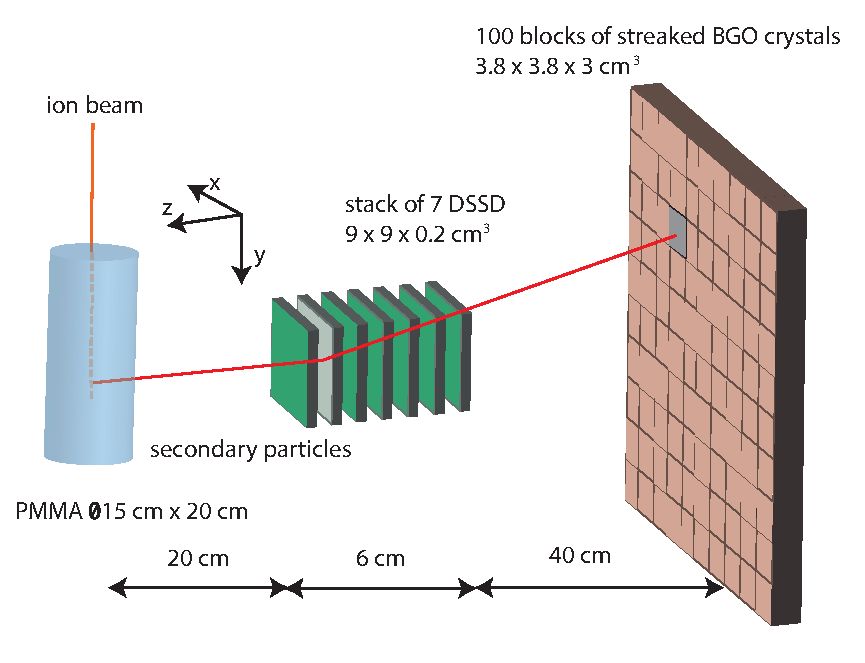
\includegraphics[width=0.7\textwidth]{03_GraphicFiles/chapter3/HT/Compton_Camera_hadontherapy_PMMA_Cylinder_EN.pdf}
  \caption{Scheme of the simulation setup (not at scale): a PMMA cylindrical phantom is set in front of the Compton camera prototype. The Compton camera is composed of a stack of 7 double sided silicon strip detectors (scatterer) and a plan of 100 single BGO blocks. The set distances are realistic for clinical conditions. This geometrical configuration has been used for all the simulations presented in this work.}
  \label{fig:fig_setup_CC_simulation_Hadronth}
\end{figure}

The silicon detectors have a strip pitch of 1.4~mm, for a total of 64 strips per side (double-sided readout based on electron and hole pairs collection). 
Regarding the BGO blocks, their entrance surface is streaked in a 8$\times$8 matrix of pseudo-pixels, $4.4\times4.4$~mm$^{2}$ size, and the readout is performed via 4 photo-multiplier tubes. The position reconstruction is achieved via Anger logic.

A scheme of the simulation setup is given in figure~\ref{fig:fig_setup_CC_simulation_Hadronth}. The ion beam interacts with a cylindrical PMMA (PolyMethylMethAcrylate) phantom (15~cm diameter and 20~cm length) placed in front of the Compton camera as target. It is placed 20~cm far from the first silicon plane (center-to-center distance) which seems a realistic distance in clinical conditions. The distance between the last silicon layer and the absorber array (center-to-center) is set to 40~cm in order to permit time-of-flight measurements (see section~\ref{MatMeth::TOF_Ecut}).

The silicon detector strips are not reproduced in the simulation code, and the transverse spatial resolution is set to 0.9~mm FWHM at the reference energy of 1~MeV, according to preliminary measurements performed on smaller detector prototypes. Concerning the transverse direction (perpendicular to the beam line), the interaction position is set to the center of the involved silicon plane. A mono-block crystal is simulated for the absorber for simplicity. The events are selected to be limited to a single block component based on the interaction localization, and the interaction position is reconstructed via center of gravity calculation if multiple interactions occur. An uncertainty contribution, randomly extracted by a Gaussian of 5~mm FWHM, is added to the reconstructed position to mimic the pseudo-pixel-based readout. For what concerns the parallel direction, given the fact that the employed BGO blocks have not depth of interaction reconstruction capabilities, the interaction position is fixed to the center of the mono-block crystal.

The energy resolution of the BGO blocks was estimated in preliminary measurements and is accordingly set to 17\% FWHM at the reference energy of 667~keV (a 137-cesium source has been used for the measurements). The energy resolution of the silicon detector is set to 5~keV (FWHM) according to the design expectations.

The time resolution has been set to 3.0~ns FWHM for the BGO blocks and to 15.0~ns FWHM for the silicon slabs, according to preliminary measurements performed on test detector modules at the GANIL %(Grand Accelerateur National d'Ions Lourds) 
center in France.

The detector resolutions play an important role in the Compton camera performances. The spatial resolution of the absorber influences the position of the apex of the Compton cone as well as its axis orientation. The energy resolution of the scatterer determines the Compton cone aperture angle. The time resolution impacts the coincidence window between the absorber and the scatterer, and therefore the detectors ability to distinguish between true and random coincidences.

The CLaRyS project also includes the development of a beam tagging hodoscope, composed of scintillating fibers read out by multi-channel photomultipliers. This detector is used to synchronize the beam time and space structure to the prompt gamma detection in order to tune the detection window reducing the background contamination. In addition to this, the spatial localization of the impinging beam bunch can be included in the event reconstruction algorithm to add constraints to the obtained solutions (see section~\ref{MatMeth:reconstruction}). The hodoscope is not included in the simulation, but its spatial and time resolution have to be taken into account for the time-of-flight discrimination (see section~\ref{MatMeth::TOF_Ecut}) and events reconstruction. They are set to 1~ns and 1~mm FWHM, respectively.\\ 
The detector's spatial, energy, and time resolutions are summarized in table \ref{table:table_resolution_detecteurs_CC_simulation_Hadronth}.

\begin{table}
\centering
%\begin{tabular}{>{\columncolor[gray]{0.9}}ccc}
\caption{Estimations of reachable resolutions with the detectors. Those resolutions are applied during the simulations.}
\begin{tabular}{cccc}
\hline
\textbf{Resolution (FWHM) at 1~MeV} & \textbf{Scatterer} & \textbf{Absorber} & \textbf{Hodoscope}\\
\hline 
\textbf{spatial [mm]	}			 &     0.9		 &  5 &	 1\\
%\hline
\textbf{energy}				&	5~keV		&  17~\%	&	/\\
%\hline
\textbf{timing [ns]}	        		&	15			&	3 	&  1\\
\hline
\end{tabular}
\label{table:table_resolution_detecteurs_CC_simulation_Hadronth}
\end{table}
    
The Monte Carlo simulation is performed with the Geant4 toolkit, version 9.6.02. 
%Geant4 has been developed at CERN %(Conseil europ\'{e}en pour la recherche nucl\'{e}aire) for high energy physics experiments, but it has been shown that it can be used for ion beam therapy studies \cite{cirrone_hadrontherapy_2011,toshito_new_2010}. 
%Some improvements are still needed in order to extend the hadronic models to low energy applications~\cite{dedes_assessment_2014, Pinto:2016aa}.
The particle interactions in matter are described in this work by means of the models listed in table~\ref{table:table_modele_physic_CC_simulation_Hadronth}. Additionally, the Doppler broadening and the photon polarization effects are included.
 

\definecolor{Gray}{gray}{0.9}

\begin{table}
\label{physlist_ion}
\caption{Hadronic models used in the Geant4 simulations.}
\begin{scriptsize}
\begin{center}
\renewcommand{\arraystretch}{1.2}
%\begin{tabular} {>{\columncolor[gray]{0.9}}cccc}\hline  
\begin{tabular} {cccc}\hline
%\rowcolor{Gray}
\textbf{Process} & \textbf{Protons} & \textbf{Ions} & \textbf{Neutrons} \\ \hline 
\textbf{Electromagnetic} & \multicolumn{3}{c}{standard$_{\rm{option3}}$} \\ %\hline
\textbf{Inelastic} & G4BinaryCascade & G4QMDReaction  &  G4BinaryCascade  \\ 
 & & (G4IonsShenCrossSection)&+ G4NeutronHPInelastic ($<$19~MeV)\\ %\hline
\textbf{Elastic} & G4LElastic & G4LElastic & G4LElastic + G4NeutronHPElastic ($<$19~MeV)\\ %\hline
\textbf{Fission} & / & / & G4LFission + G4NeutronHPFission($<$19~MeV) \\ %\hline
\textbf{Capture} & / & / & G4LCapture +  G4NeutronHPCapture ($<$19~MeV) \\ %\hline
\textbf{Radioactivedecay} & / & G4Radioactivedecay & / \\ \hline
\end{tabular}
\end{center}
\end{scriptsize}
\label{table:table_modele_physic_CC_simulation_Hadronth}
\end{table}

%\subsection{Data processing}
%\label{subsection:Treatment_data_CC_hadrontherapy_Geant4}

\subsection{Beam structure}
\label{subsection:modelisation_fasceau_ions_CC_hadrontherapy_Geant4}
\subsubsection{Beam structure measurements at HIT}\label{beam_measurement}
Our group performed a set of measurement to characterize the beam time structure of the synchrotron installed in the Heidelberg Ion Therapy Center (HIT), Germany~\cite{HIT_timestructure}. This set of measurements extends the results reported in~\cite{HIT_timestructure} and is then used to reproduce a realistic beam in the simulation.\\
The beam characterization has been performed for 200~MeV/u and 400~MeV/u primary ion energy with a two-fiber hodoscope (basic prototype of the one at present under development) and the spill signal was given by the accelerator. Figure \ref{fig:fig_structure_temps_faisceau_HIT_2013_CC_simulation_Hadronth} shows the results for carbon ions at 400~MeV/u. The pulses have a spill period of 150.2~ns and each bunch is approximately 21.5~ns.
The mentioned measurements have shown that the spill phase changes during the extraction: this implies that the HF signal from the synchrotron can not be used to trigger the pulses, so that the use of an additional beam time stamp system like the hodoscope seems required for time-of-flight background rejection purposes.

\begin{figure} [!hbtp]	
  \centering
  %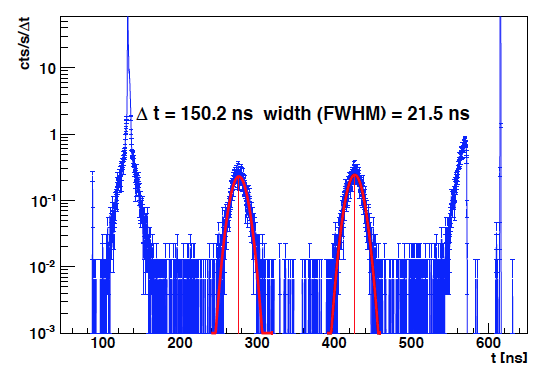
\includegraphics[width=0.6\textwidth]{./Figure/2013_Structure_Time_Beam_400MeV.png}
  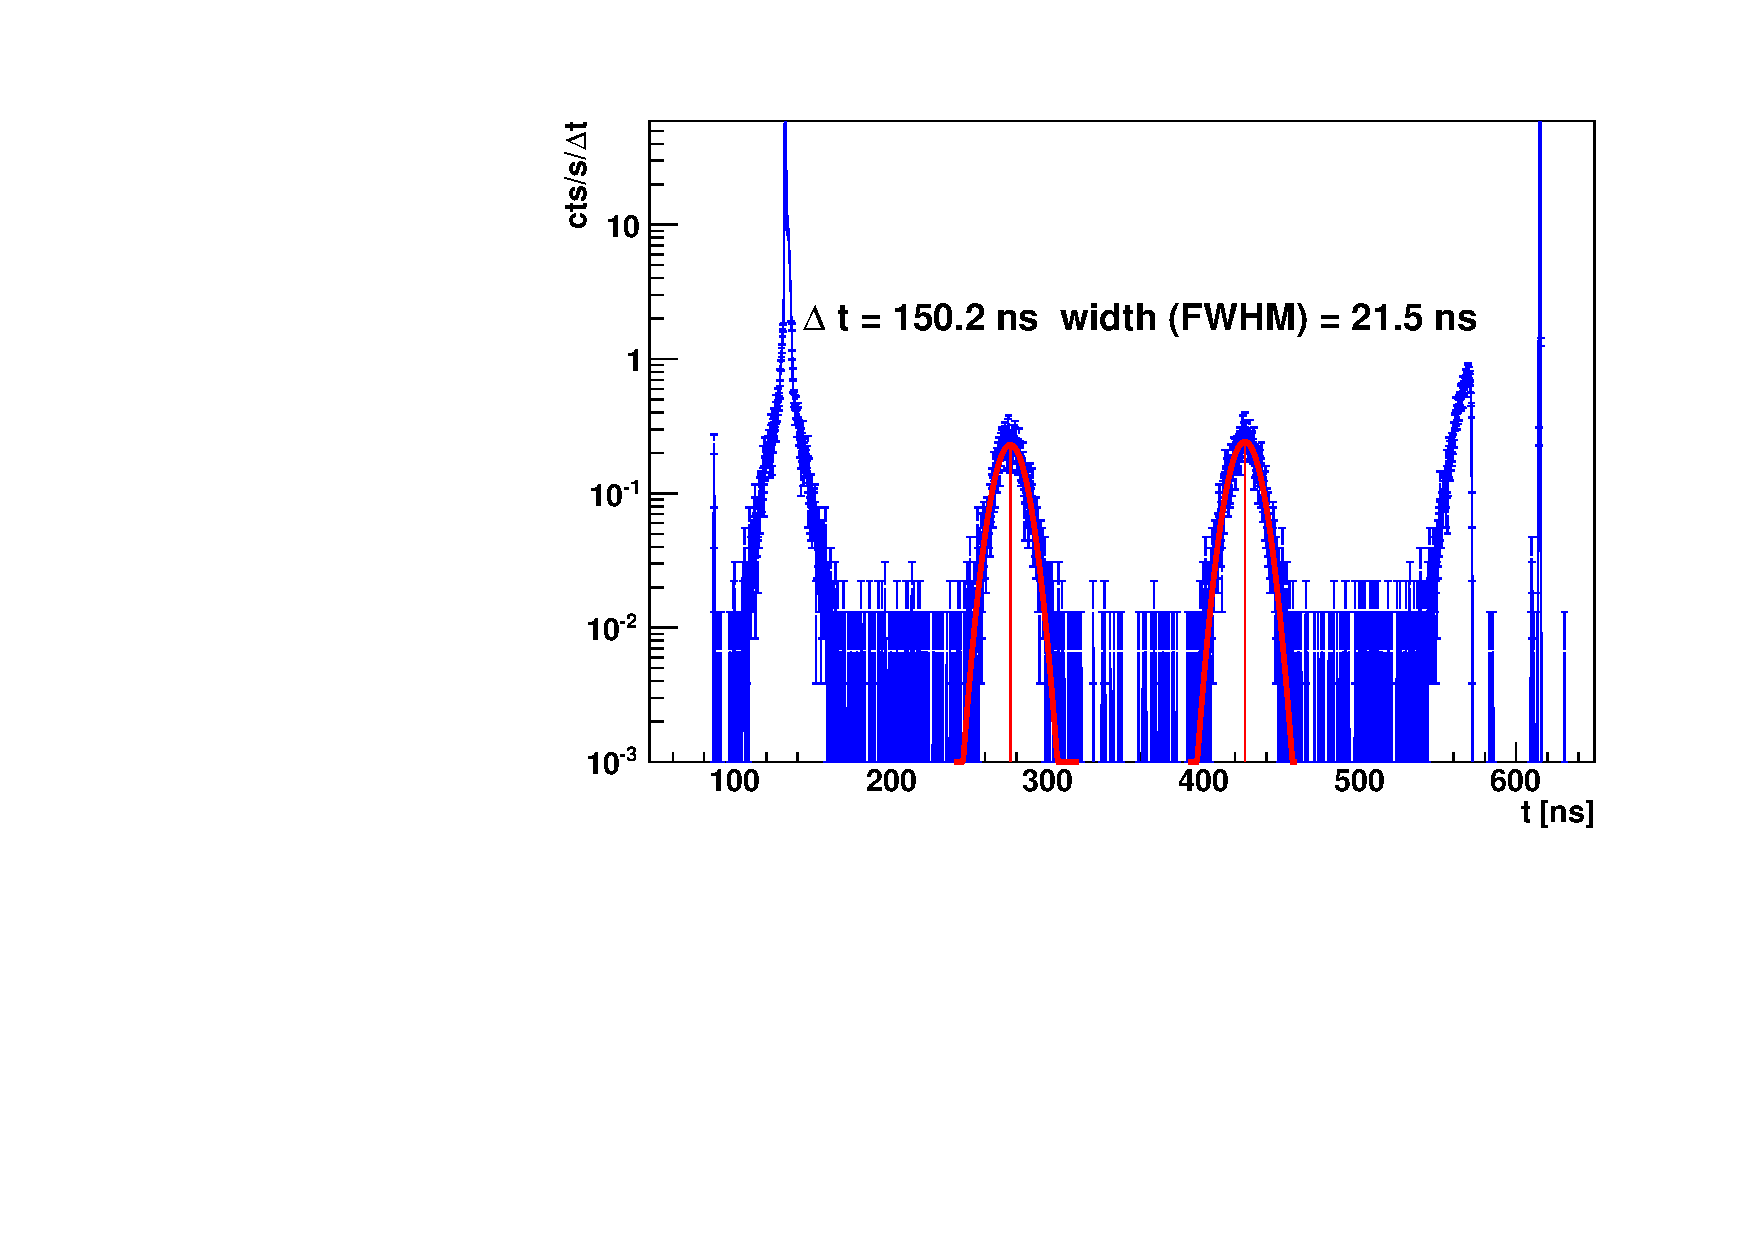
\includegraphics[width=0.6\textwidth]{03_GraphicFiles/chapter3/HT/fiber_vert_hor_run14.pdf}
  \caption{Time micro-structure measured from a carbon ion beam at 400~MeV/u delivered at HIT. The pulses have an extraction period of 150.2~ns and the bunches are 21.5~ns FWHM.  On the x axis the time has been measured with a two-scintillating-fiber hodoscope, with 1~ns FWHM time resolution.}
  \label{fig:fig_structure_temps_faisceau_HIT_2013_CC_simulation_Hadronth}
\end{figure}


\subsubsection{Beam modeling}\label{beam_modeling}
The two main beam particles used in clinics are considered in the simulation: protons and carbon ions. The beam range of interest is 15.2~cm in the PMMA phantom, and the associated energy is 160~MeV for protons and 305~MeV/u for carbon ions.\\ 
The beam transverse dimension is modeled with a Gaussian distribution with a standard deviation of 5~mm for protons at 160~MeV and 3.5~mm for carbon ions at 305~MeV/u. The number of incident ions for a spot in pencil beam scanning (PBS) mode is $10^8$ for protons (distal spot - upper intensity limit) and $10^5$ for carbon ions (average spot intensity)~\cite{Kramer:2000aa, Grevillot_2011,smeets_2012}. In the simulation, the beam intensity is modeled by an average number of particles per bunch. The exact number of particles in each bunch is given by a random extraction from a Poisson distribution, where the mean value is the selected beam intensity.\\
The beam time structure is applied at the data analysis stage. Two different time structures have been considered for this study, related to two kinds of accelerators used in clinical practice: the IBA C230 cyclotron for protons (used in 16 clinical centers worldwide) and the HIT synchrotron for carbon ions. For protons at 160 MeV, the primary particles are grouped in bunches of 2~ns (this value may vary also according to the distance between the cyclotron and the treatment room, and energy spread selection) at a frequency of 106~MHz (9.42~ns)~\cite{Roellinghoff_2014}. The clinical beam intensity is 3.2~nA which corresponds to about 200 protons per bunch. Concerning the carbon ion beam at 305~MeV/u, the simulated time structure refers to the measurements presented in section~\ref{beam_measurement}. We used 30~ns duration bunches a frequency of 5.9~MHz (170~ns period). The clinical beam intensity for carbon ions is $5\times10^7$~ions/s during extraction, corresponding to about 9~ions per bunch. 

The coincidence window (between scatterer and absorber events) is set to 40~ns, centered on each absorber detected interaction. This value is adapted to the detectors time resolutions. At the simulation stage, each interaction in the detector layers is collected with the related local time. The beam time structure is then applied to each single hit, and the selected coincidence window is used to retrieve scatterer-absorber coincidence events.\\ 
Table~\ref{table:definition_beam_structure_CC_hadrontherapy_Geant4} summarizes the presented beam time structures and coincidence reconstruction features.

\begin{table} [!htbp]
\footnotesize
\centering
\caption{Description of the two beam structures studied: the IBA cyclotron C230 for protons and the synchrotron installed at the Heidelberg Ion Therapy Center (HIT) in Germany for carbon ions. The macro-structure of the synchrotron, at the second time scale, is not considered here. The beam structures are applied to the simulation data.}
\setlength{\tabcolsep}{2pt}
%\hspace{-2.1cm}
\begin{tabular}{c|c|cc}
%\cline{2-4}
\hline
		\multicolumn{2}{c}{ }		 & 					\textbf{Protons} & \textbf{Carbon ions}\\ 
\hline
%\cline{2-4}%\hline
\multirow{3}{*}\textbf{Clinical features}		&	Facility	& IBA Cyclotron C230 &   Synchrotron at HIT\\
											& Clinical intensity& $  2\times10^{10}$ p/s  & $  5\times10^{7}$ ions/s\\
											& Energy 			&160~MeV 			&    305~MeV/u\\
%\cline{2-4}%
\hline
\multirow{3}{*}\textbf{Beam structure}		&	Bunch time [ns]	& 3.2				&  30\\
											& Period [ns]		&   9.4 				& 170\\
											& Primaries/bunch 	&217 			& 9\\
%\cline{2-4}%
\hline
\multirow{2}{*}\textbf{Detectors}						& Coincidence window [ns]		& 40 	&  40 \\
											&Time resolution (FWHM) [ns] & \multicolumn{2}{c}{Si: 15 and BGO: 3}\\
%\cline{2-4}%
\hline
\end{tabular}
\label{table:definition_beam_structure_CC_hadrontherapy_Geant4}
\end{table}



%\newpage
%---------------------------------------------------------------
%---------------------------------------------------------------
\subsection{TOF and energy based data selection}
\label{MatMeth::TOF_Ecut}

The Compton detection principle is based on a double interaction in the scatterer and absorber section, where an interaction is defined as an energy deposit in a detector module. As discussed in section~\ref{subsection:modelisation_fasceau_ions_CC_hadrontherapy_Geant4}, the coincidence reconstruction relies on a defined time window, fixed according to the detector resolution. In a simulation environment, different kinds of coincidence events can be distinguished and studied: 
\begin{itemize}
\item[-] real coincidences: created by a single photon first interacting in a single scatterer plane and then in a single absorber block;
\item[-] quasi-simultaneous interaction of two secondary particles;
\item[-] double interaction of the same particle, not a photon (e.g. protons, neutrons).
\end{itemize}

In an experiment the collected data are affected by a certain number of the so-called random coincidences, which cannot be experimentally distinguished from true coincidences, from the timing coincidence point of view. The amount of random coincidences depends on the detector time resolutions, the fixed time coincidence window and the beam time structure, the phantom composition and camera prototype setup. In figure~\ref{fig:fig_explication_coincidence_CC_simulation_Hadronth}, a schematic view of the different kinds of coincidences is presented.

\begin{figure}
  \centering
  \includegraphics[width=0.9\textwidth]{03_GraphicFiles/chapter3/HT/Schema_coincidence_EN.eps}
  \caption{Diagram showing the different definitions of coincidences in the Compton camera.}
  \label{fig:fig_explication_coincidence_CC_simulation_Hadronth}
\end{figure}

In addition to this, the prompt gamma measurement is contaminated by other secondary particles (mainly massive and charged particles like protons and neutrons), produced by the interaction of the primary particles with the patient/phantom.
Ad-hoc filtering methods are applied to reduce the above described contamination.

\begin{itemize}
\item Time-Of-Flight: it has been demonstrated that a time-of-flight discrimination is possible and effective in reducing the background generated by massive particles interactions~\cite{Testa:2010aa}. The massive particles approach the detector at a lower speed with respect to photons. The time information provided by the hodoscope and the absorber can be combined to fix a detection time window and reject all the events outside the window. The time elapsed between the incident particle creation ($\mathrm{t_{creation}}$) and the secondary particle detection in the absorber ($\mathrm{t_{absorber}}$) is considered as the time-of-flight. The particle creation time is modeled according to the beam time structure, as presented in section~\ref{beam_modeling}. The detection time in the absorber is calculated with the simulation local time of the hit in the detector layer. The hodoscope time resolution (1~ns FWHM) is applied to the primary particle creation time, with a contribution randomly extracted from a Gaussian with $\sigma\,=$ 1/2.35~ns ($u_{\mathrm{hodoscope}}$) . The detection time in the absorber is affected by the absorber time resolution, already included in the simulation code.

 \begin{eqnarray}
%TOF = t_{\mathrm{absorber}}-t_{\mathrm{hodoscope}} \\
TOF_{\mathrm{simulation}} = t_{\mathrm{absorber}}-(t_{\mathrm{creation}} + u_{\mathrm{hodoscope}})
\label{TOF_equation}
\end{eqnarray} 

The time-of-flight spectrum resulting from the simulation shows that the coincidences of interest (produced by prompt-gamma rays) are included in a window between 0 and 8~ns (figure \ref{fig:fig_TOF_distribution_CC_simulation_Hadronth}). Therefore, all the coincidences with a TOF no included in this time window have been rejected.
\begin{figure}	
  \centering
  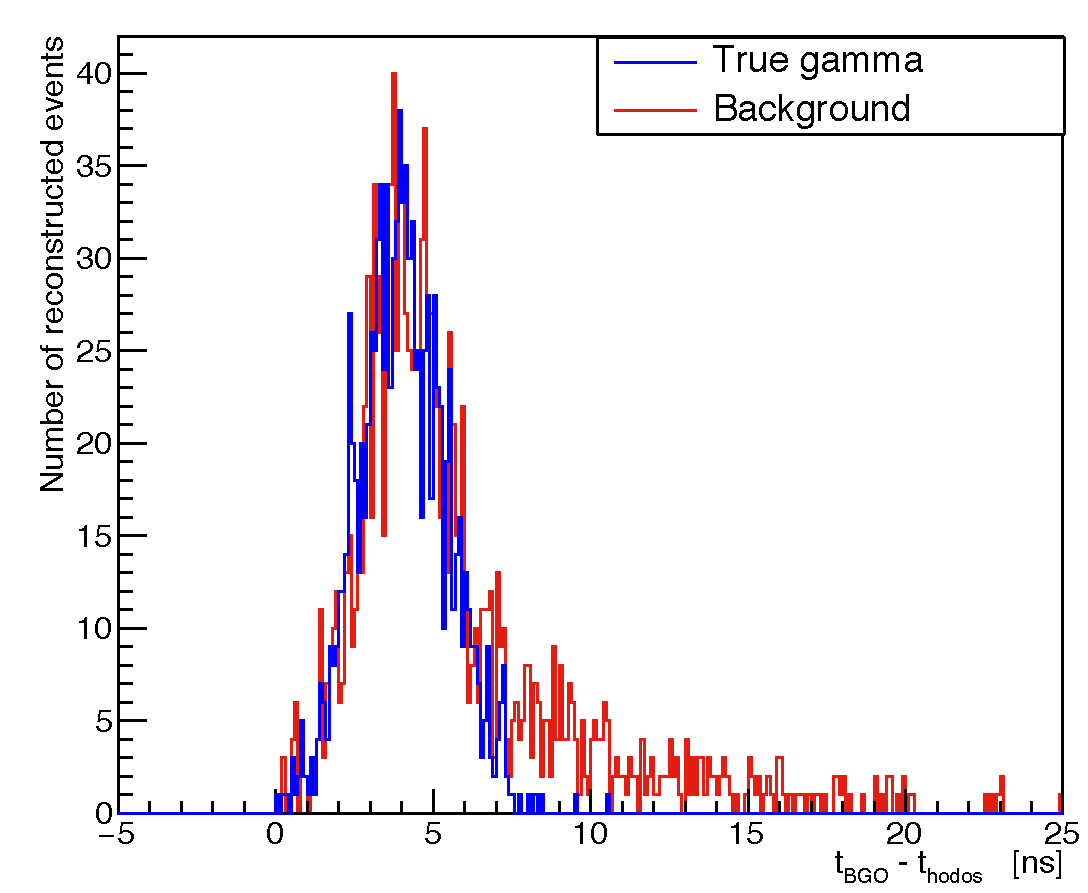
\includegraphics[width=0.6\textwidth]{03_GraphicFiles/chapter3/HT/TOFspectra_2}
  \caption{Time of flight spectra of true gamma coincidences (blue) and background events (red) obtained with $10^{8}$ 160~MeV incident protons.}	
  \label{fig:fig_TOF_distribution_CC_simulation_Hadronth}
\end{figure}

\item Energy selection: energy thresholds are defined for the event detection. 50~keV and 100~keV are set as lower threshold for the energy deposited in a single silicon layer and absorber, respectively. For a complete event, a total absorbed energy lower limit is set to 1~MeV. In addition to the effect of background rejection, this selection also reduces the impact of partially absorbed photons and events with Compton electron escape.

Further energy selections, assuming for instance $E_1+E_2$ equal to one of the strong gamma lines, have been applied by other authors. Also, filters checking the possibility of reconstructing a Compton cone could be used. At this stage we did not consider such approaches, in order to cope with simple considerations on signal to noise on raw data.

\end{itemize}

\subsection{Reconstruction algorithms}
\label{MatMeth:reconstruction}
Once the coincidences are defined and selected according to the fixed physical cuts, the prompt-gamma emission point has to be reconstructed for each event. This can be done via analytic or iterative algorithms based on the Compton kinematics. Both are presented in the following sections.


\subsubsection{Line-cone algorithm}
The reconstruction via line-cone algorithm exploits the energy deposit and position information collected by the camera in addition to the beam spatial information provided by the hodoscope. Thanks to the deposited energies in the detectors and the interaction positions, a cone surface is analytically defined via the Compton equation~\ref{Compton_equation}. Figure~\ref{fig:reconstruction_scheme} shows a sketch of the reconstruction principle. The interaction position in the scatter gives the cone apex and the line connecting the interaction positions in scatterer and absorber gives the cone axis. We assume that the initial energy of the gamma ray is fully absorbed in the absorber. According to previous simulation results, the rate of events fully absorbed in the Compton camera is more than 60~\% in the PG energy range. In order to constrain the reconstruction, the beam direction is used to limit the possible solutions (lying on the reconstructed cone surface) to two points (intersection of the beam direction and the reconstructed cone). The set of all the reconstructed points gives the emission source distribution. The final image is the mono-dimensional projection of the prompt gamma emission spectrum. 

\begin{figure}
\centering
  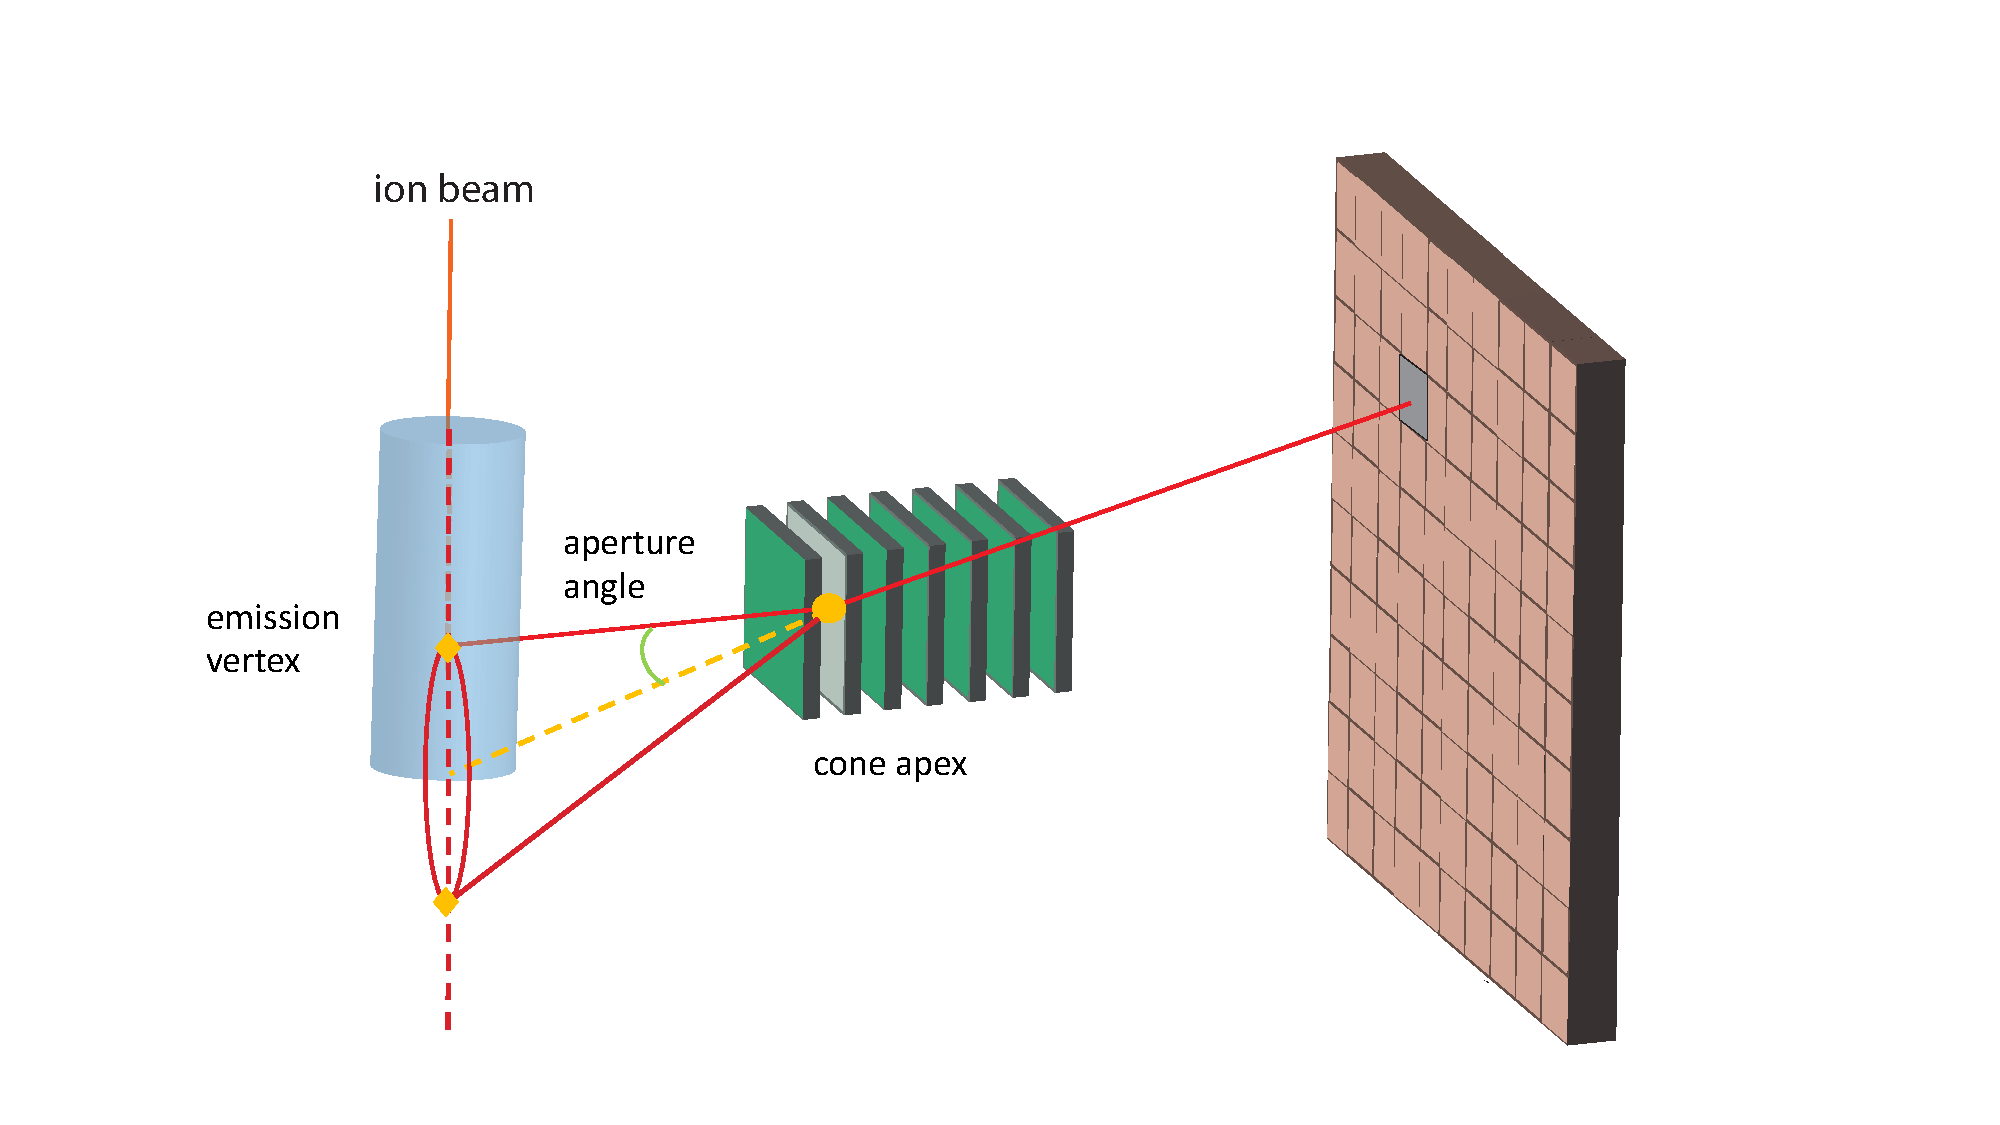
\includegraphics[width=0.8\textwidth]{03_GraphicFiles/chapter3/HT/reconstruction_scheme}
  \caption{Scheme of the reconstruction principle for Compton events. For line-cone reconstruction methods, two points are extracted for each event (diamonds in the figure), provided by the intersection between the reconstructed Compton cone and the beam line. The reconstructed image is strictly 1D. For the iterative MLEM algorithm, each algorithm iteration adds constraints to the reconstructed cone surfaces, leading to  a 3D image.}	
  \label{fig:reconstruction_scheme}
\end{figure}

\subsubsection{LM-MLEM algorithm}	
The iterative methods allow to get a 3D image reconstruction, potentially by taking into account the spatial resolution and the energy resolution of the detectors. Few iterative algorithms have been developed for Compton event reconstruction~\cite{schone_common_2010, zoglauer_design_2011,gillam_compton_2011,mackin_evaluation_2012,lojacono_low_2013}.

The \textit{List-Mode Maximum Likelihood Expectation Maximization} (LM-MLEM) algorithm is an MLEM version which allows to reconstruct the image directly from the list of detected events.
The LM-MLEM algorithm used for this study is detailed in~\cite{hilaire_compton_2014}.%\cite{maxim_filtered_2014,hilaire_compton_2014}.%\cite{maxim_analytical_2009,lojacono_low_2013,maxim_filtered_2014,hilaire_compton_2014}.\newline

%The first step is to define the volume which includes the origin of the prompt gamma ray detected. This volume is divided into equal voxels and the emission intensity is assumed homogeneous for each voxel $j$, with a Poisson distribution of parameter $\lambda_j$ (a vector of the emissions intensities of all the voxels). The algorithm is based on a system matrix $T$ composed of the coefficients  $t_{ij}$ which represent the probability that a photon produced in the voxel $j$ is detected in coincidence by the Compton camera as an event $i$. The probability for a gamma detected in coincidence to be emitted from the voxel $j$ is denoted as $s_j$.
%The LM-MLEM algorithm starts with an initial value $\lambda^{(0)}_j$, which can be the simple back-projection reconstruction.
%The iterations rely on the following recurrence relation:
%
%\begin{equation}
%\lambda_j^{(l+1)} =  \frac{\lambda_j^{(l)} }{s_j} \sum\limits_{i=1}^{N_{\gamma}} t_{ij} \frac{1}{P_i^{(l)}},\quad \rm{with}\quad  P_i^{(l)}=\sum\limits_{k=1}^{N_{v}} t_{ij}\lambda_k^{(l)},
% \label{eq:equation_lambda_compton_med_nucleaire}
%\end{equation}
%where $N_{\gamma}$ is the number of detected events and $N_v$ is the number of voxels in the image.
%
%For each photon detected, the coefficients in column i are calculated by taking into account the uncertainties on the angle between the source and the involved scatterer plane and the angle between the scatterer plane and the absorber involved module.
%The matrix elements $t_{ij}$ are calculated as:
%\begin{equation}
% t_{ij} = K(\beta_i,E_{tot})\frac{|\rm{cos}(\theta_{{V_2V_1}}) |}{V_2V_1^2} \int\limits_{M\in v_j} \frac{|\rm{cos}(\theta_{V_1M})|}{V_1M^2} h_i(M)dv,
% \label{eq:equation_tij_compton_med_nucleaire}
%\end{equation}
%where $\beta_i$ is the Compton scattering angle, $V_1$ the interaction position in the scatterer, $V_2$ the interaction position in the absorber, $h_i$ the spatial kernel which models the uncertainties on the Compton angle for each voxel $M$, $K(\beta_i,E_{tot})$ the differential cross section and $v_j$ the reconstructed volume.
%
%In order to simplify and speed up the calculation of the $t_{ij}$ matrix, the voxels located far from the reconstructed cone are set to 0. The distance between the cone and the voxel is calculated by taking the voxel center as reference point. %The spatial resolutions are not included in this version of the algorithm.\newline
%For each iteration, the matrix $T$ is stored and the reconstructed image can be produced.


\subsection{Performance study}
\label{MatMeth:performance}
In this section the parameters studied for the camera performance evaluation are explained. The study is mainly divided into three sections:
\begin{itemize}

\item Absolute efficiency: the camera absolute efficiency for gamma detection is studied by means of mono-energetic irradiation with point-like sources;
\item Rate of random coincidences: with proton and carbon beams interacting with the PMMA phantom, the rate of random and true detected coincidences is studied as a function of the beam intensity;
\item Camera precision: the camera capability of identifying the fall-off of the prompt-gamma emission profile is tested and the two reconstruction methods presented above are compared. 

\end{itemize}


\subsubsection{Absolute detection efficiency}
The absolute efficiency is crucial for the Compton camera performances and for its possible application in treatment monitoring. An efficient monitoring system should be ideally in real time, in order to allow for a treatment adaptation or interruption in case of severe issues detected in the delivered dose profile with respect to the planned treatment. In order to achieve an online detection of such deviations, given the limited prompt gamma emission rate per incident ion~\cite{Ortega:2015aa}, a high detection efficiency is required to perform a monitoring on, ideally, a beam spot basis. In addition to this, the absolute detection efficiency directly affects the image reconstruction quality, which is in general increased for increased statistics.

In order to well define the expected camera efficiency, it has been studied with the irradiation from point-like mono-energetic gamma sources, set in different positions with respect to the center of the camera on the transverse plane.	

The absolute efficiency $\epsilon$ is defined as:
\begin{equation}
\epsilon =\frac{\mathrm{N}\gamma_{\mathrm{coinc}}}{\mathrm{N}\gamma_{\mathrm{total}}},
\end{equation}
\label{eq:equation_efficacite_absolue}
with $N\gamma_{\mathrm{coinc}}$ the number of gamma events corresponding to true coincidences, $N\gamma_{\mathrm{total}}$ the total number of emitted gammas.

The setup is the same as figure~\ref{fig:fig_setup_CC_simulation_Hadronth}, with the exception of the PMMA phantom which is removed to leave the gamma source in air.
The point-like source is set in the range $-300$~mm to $+300$~mm (with the center of the camera transverse section set in the position 0), and moved in variable length steps: 20~mm close to the center of the camera, then increasing up to 1~cm for the most peripheral point. The movement followed the transverse axis of the camera. Different energies have been tested to mimic different prompt gamma lines: 300~keV, 500~keV, 1~MeV, 2~MeV, 4~MeV, 6~MeV. No time structure is reproduced for this part for the study.\\
Moreover, the rate of events with a almost full primary energy absorption has been studied as a function of the primary gamma energy and the position in the range presented above. The threshold for the energy absorption has been set to 90\% of the primary gamma energy.\\ 

\subsubsection{Rate of random coincidences}

As the Compton detection principle relies on time coincidences, in addition to the main importance played by the detectors energy resolutions, the beam intensity and time structure are important parameters to be studied in order to assess the possible clinical implementation of a Compton detection based monitoring of ion beam treatment. The ability of the detection system to distinguish between true and random coincidences, i.e.~the resulting signal over noise ratio, strongly depends on the beam time structure. The number of true and random coincidences (where the two cases listed in section~\ref{MatMeth::TOF_Ecut} are included in the random coincidences) is studied as a function of the beam intensity, before and after data reconstruction via line-cone algorithm~(see section~\ref{MatMeth:reconstruction}).

The range of intensities is defined in order to cover a wide range of operation: from a very low beam intensity to a realistic clinical particle rate. Therefore, for proton and carbon ions, the lowest beam intensity is set to 0.1 particles per bunch on average, while the upper limit is set to 217 protons or 70 carbon ions per bunch. All the simulations are performed with a total of $10^{8}$ primary protons and  $2\times10^{5}$ primary carbon ions (see section~\ref{beam_modeling}). For the analysis of the results, the coincidence yields are scaled to the number of incident ions and the beam intensity to the average number of ions per bunch.

\subsubsection{Camera precision}
\label{MatMeth:precision}

The camera precision is defined as the difference between the predicted PG fall-off position - FOP - (according to the treatment planning) and the detected one.
In this study, a reference profile has been defined as the reconstructed emission vertex profile at high statistics ($\mathrm{10^{10}}$ incident protons). This Bragg peak position is used as reference and compared to the ones at lower statistics, deduced as described in the following.

For the LM-MLEM reconstruction, the reconstruction volume is set to $20\times40\times1$~cm$^3$ around the expected FOP, with a $100\times200\times5$ voxel matrix. To be noticed that the two reconstruction methods produce different results: the line-cone method is based on the beam direction information, so that it naturally returns a mono-dimensional image as result, while the LM-MLEM method is able to reconstruct the prompt-gamma emission distribution in three dimensions. A mono-dimensional projection along the beam direction is used for the falloff identification and for a direct comparison of the line-cone method.
The \textit{SmoothKern} method, with the Nadaraya-Watson regression~\cite{Nadaraya_regression, Watson_regression}, is used to smooth the reference profiles in order to reduce relative statistical fluctuations.

A region of interest (ROI) ranging from $y=0$ mm to $y=+100$ mm is defined around the expected Bragg peak position, located at $y=+50$~mm in the phantom. The reference reconstructed profiles are modeled in the ROI by a linear combination of Non-Uniform Rational Basis Splines (NURBS)~\cite{NURBS}. 

The reference data set is normalized in order to obtain lower statistics profiles, in the range 1$\times$10$^8$ to 5$\times$10$^9$. Statistical fluctuations, randomly extracted following a Poisson law, are added to the obtained PG profiles to mimic realistic reconstructed profiles. This method is used to reduce the analysis time.

For each chosen statistics, 1000 PG profiles are generated and a custom minimization method is applied to deduce the minimal shift between the reference profile and the one at lower statistics. The minimization algorithm shifts the reference profile in a 60~mm range, between $-30$~mm and $+30$~mm with respect to the initial position, with a step of $0.1$~mm, and for each position it compares its position to the low statistics profile by calculating the $\chi^2$ as follows:
\begin{eqnarray}
\chi^2 = \sum\limits_{i=1}^{N_{bin}} {(y_{\mathrm{sample,i}}-y_{\mathrm{NURBS,i}})^2},
\end{eqnarray}
where for every bin $i$ $y_{\mathrm{sample}}$ is the number of events in the low statistics profile, $y_{\mathrm{NURBS}}$ is the number of events for the reference profile NURBS (scaled at the same low statistic). Several minimization algorithms are available, but in order to avoid artifacts at low statistic, a robust custom defined approach has been preferred.

%Figures~\ref{fig:fig_Results_Chi2_Distribution_Variation_CC_simulation_Hadronth_LC} and~\ref{fig:fig_Results_Chi2_Distribution_Variation_CC_simulation_Hadronth_MLEM} show the distribution of $\chi^2$ calculated for a low statistic profile at $10^8$ incident protons.

The global minimum of all the calculated $\chi^2$ is then retrieved and the shift associated to this value is added to the shift distributions. % shown in figure~\ref{fig:fig_Results_Precision_Distribution_Variation_CC_simulation_Hadronth_LC} and~\ref{fig:fig_Results_Precision_Distribution_Variation_CC_simulation_Hadronth_MLEM} for the line-cone and LM-MLEM algorithm respectively, for $10^8$ incident protons. 
The standard deviation of the distribution resulting of the thousand results gives the precision of the camera for a given number of incident protons. 



% \begin{figure}
% \centering
% \subfloat[\label{fig:fig_Results_Estimation_Camera_Profil_highStat_CC_simulation_Hadronth_LineCone}]{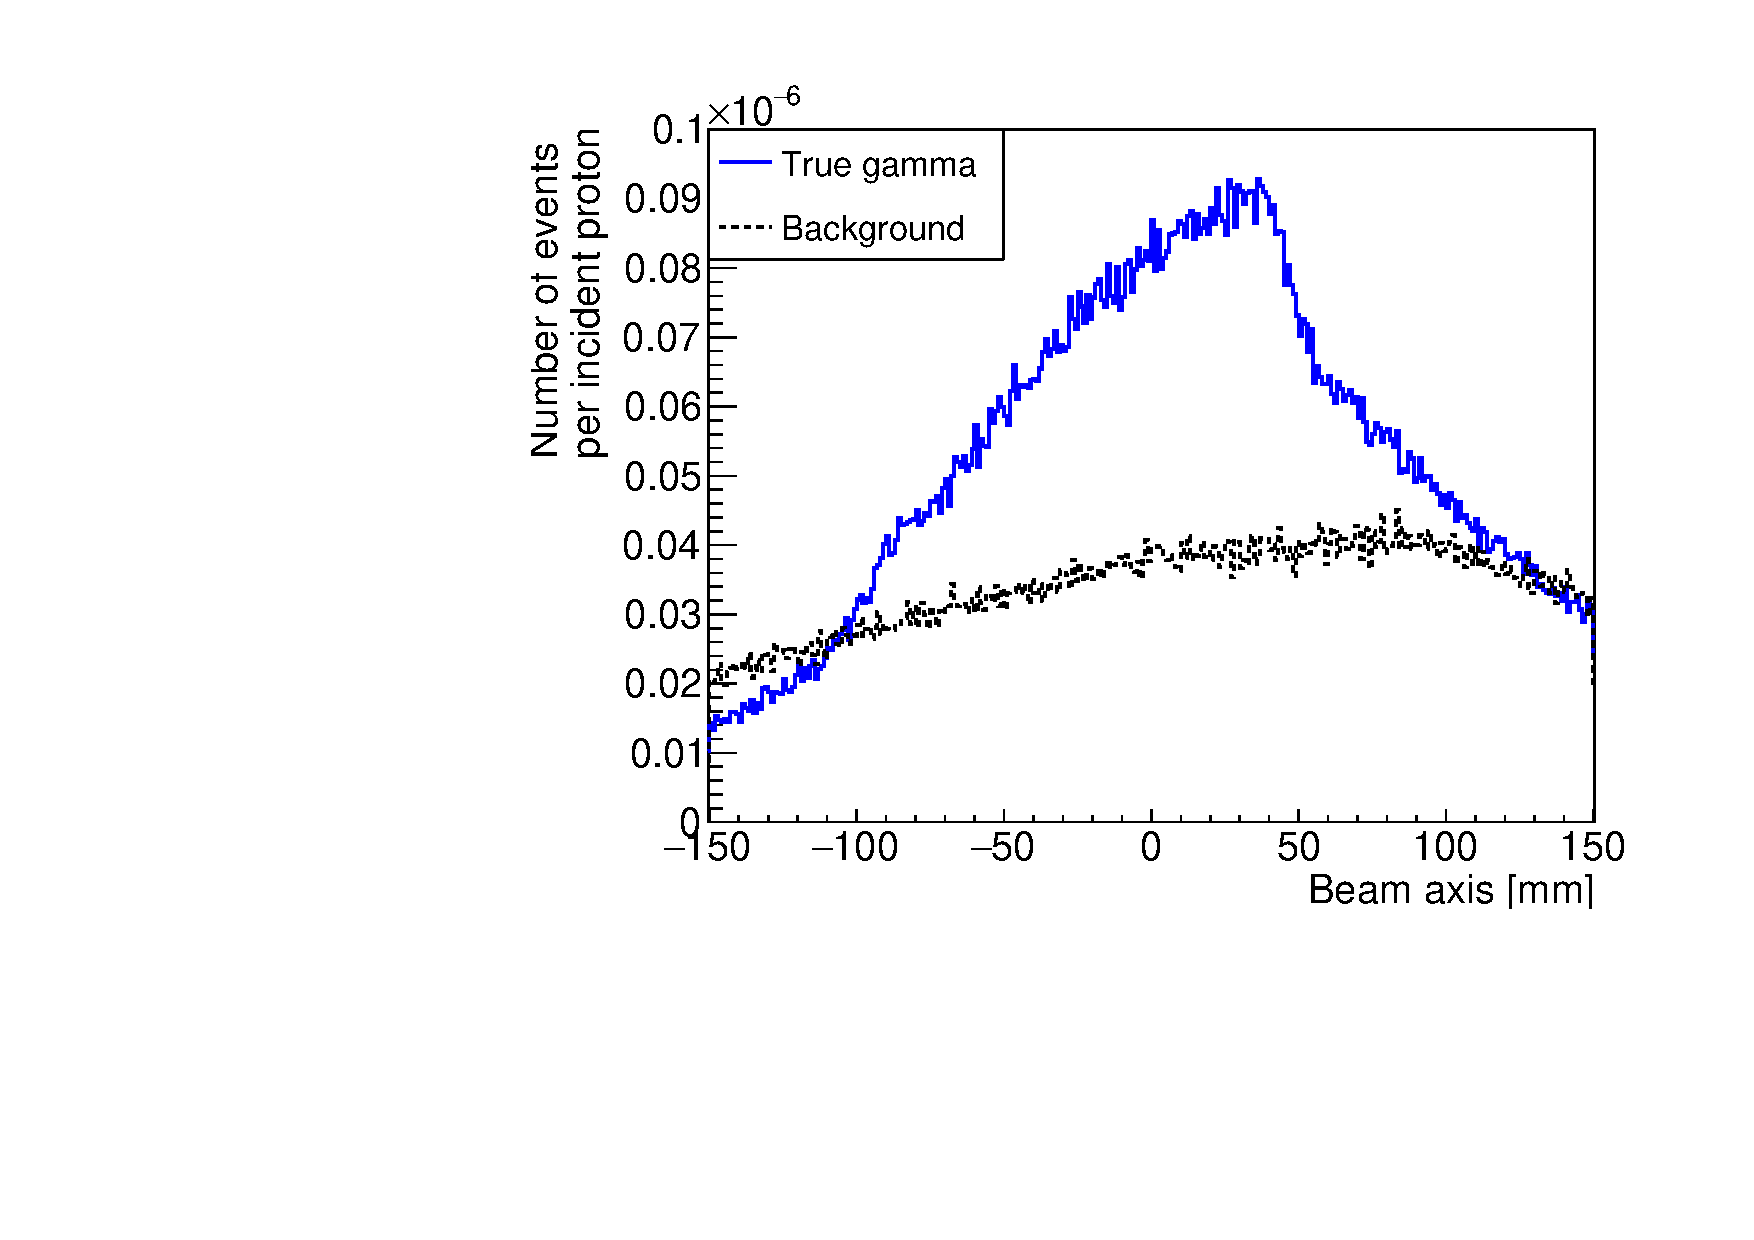
\includegraphics[width=0.33\textwidth]{./Figure/profile_high_stat_linecone_2.pdf}}
% \subfloat[\label{fig:fig_Results_Estimation_Camera_Profil_highStat_CC_simulation_Hadronth_MLEM}]{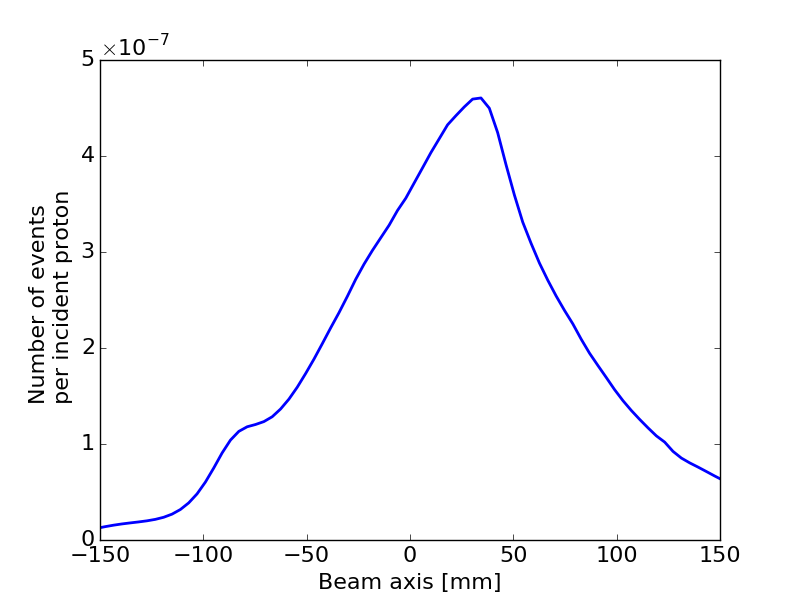
\includegraphics[width=0.32\textwidth]{./Figure/profileY_corr_r15.png}}\\
%  %\subfloat[\label{fig:fig_Estimation_Camera_CC_NURBS_Poisson_LC}]{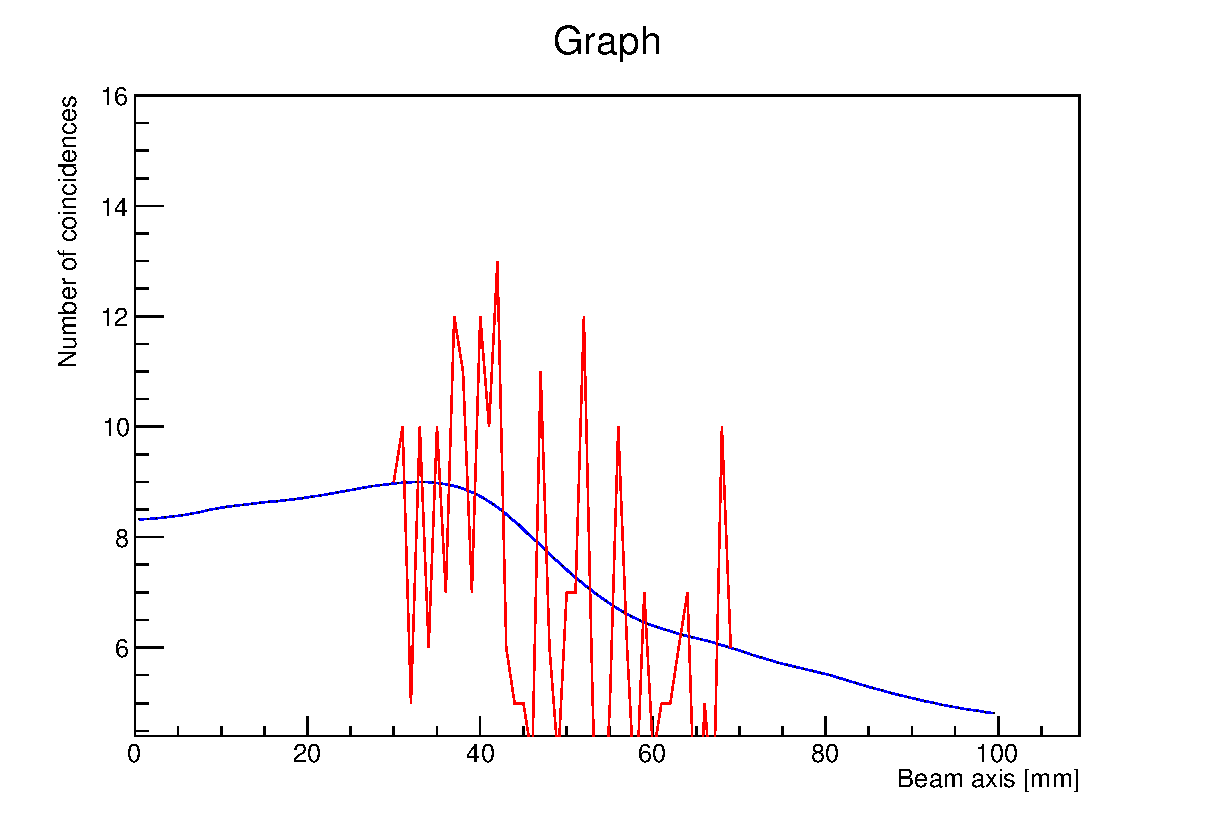
\includegraphics[width=0.33\textwidth]{./Figure/2017-08-02_Poisson_Nurbs_1e8_Article_LC.eps}}
%  \subfloat[\label{fig:fig_Estimation_Camera_CC_NURBS_Poisson_LC}]{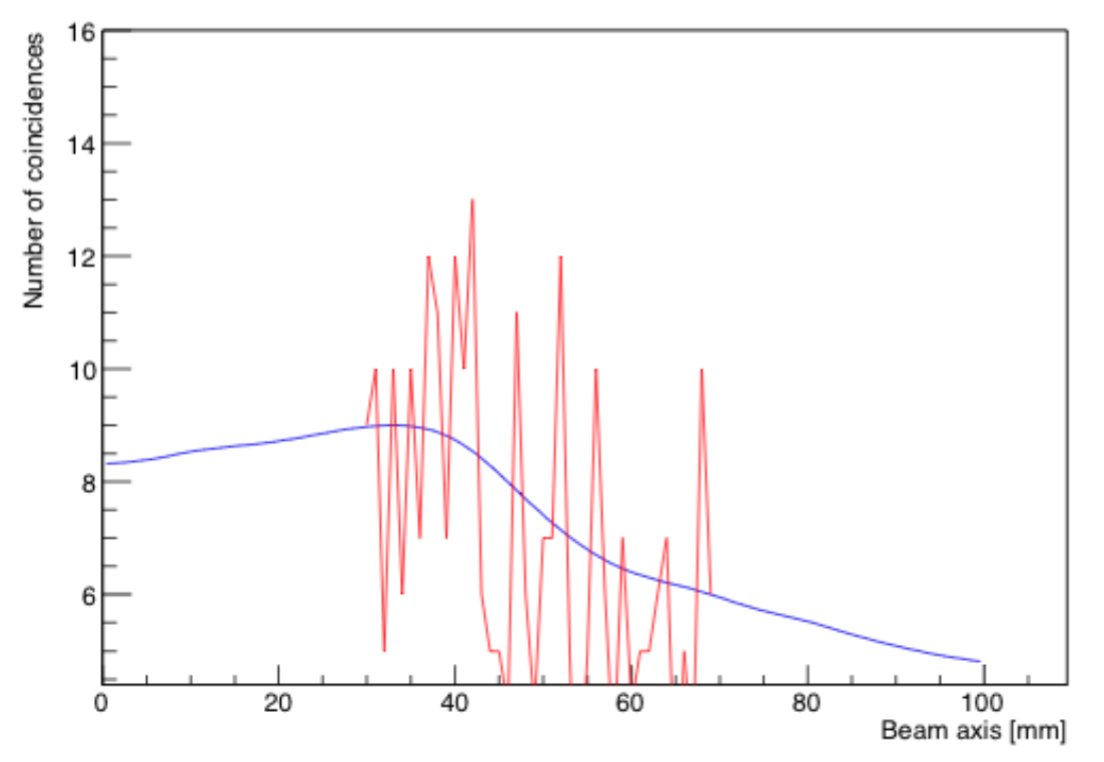
\includegraphics[width=0.33\textwidth]{./Figure/line_cone_NURBS.png}}
%  %\subfloat[\label{fig:fig_Estimation_Camera_CC_NURBS_Poisson_MLEM}]{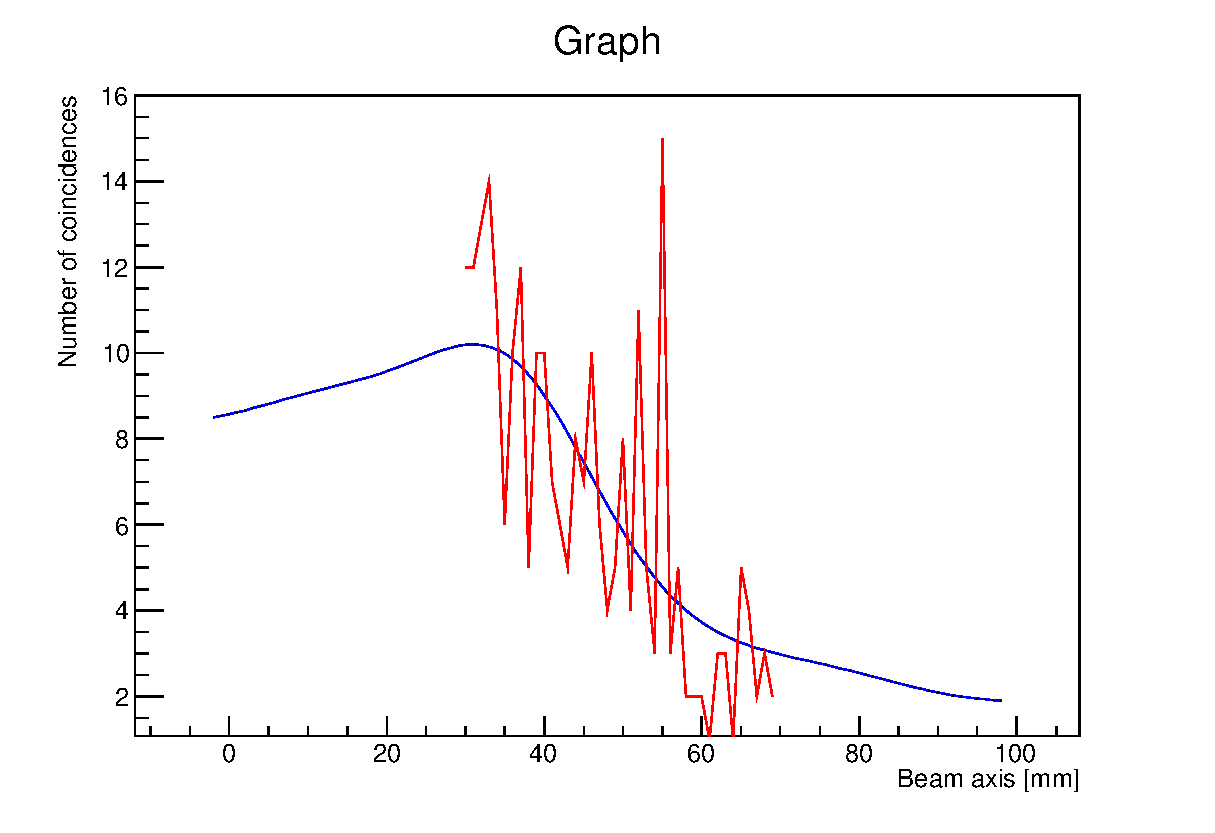
\includegraphics[width=0.33\textwidth]{./Figure/2017-08-02_Nurbs_Poisson_1e8_Article_MLEM.eps}}\\
%  \subfloat[\label{fig:fig_Estimation_Camera_CC_NURBS_Poisson_MLEM}]{\includegraphics[width=0.33\textwidth]{./Figure/MLEM_NURBS.png}}\\
%   %\subfloat[\label{fig:fig_Results_Chi2_Distribution_Variation_CC_simulation_Hadronth_LC}]{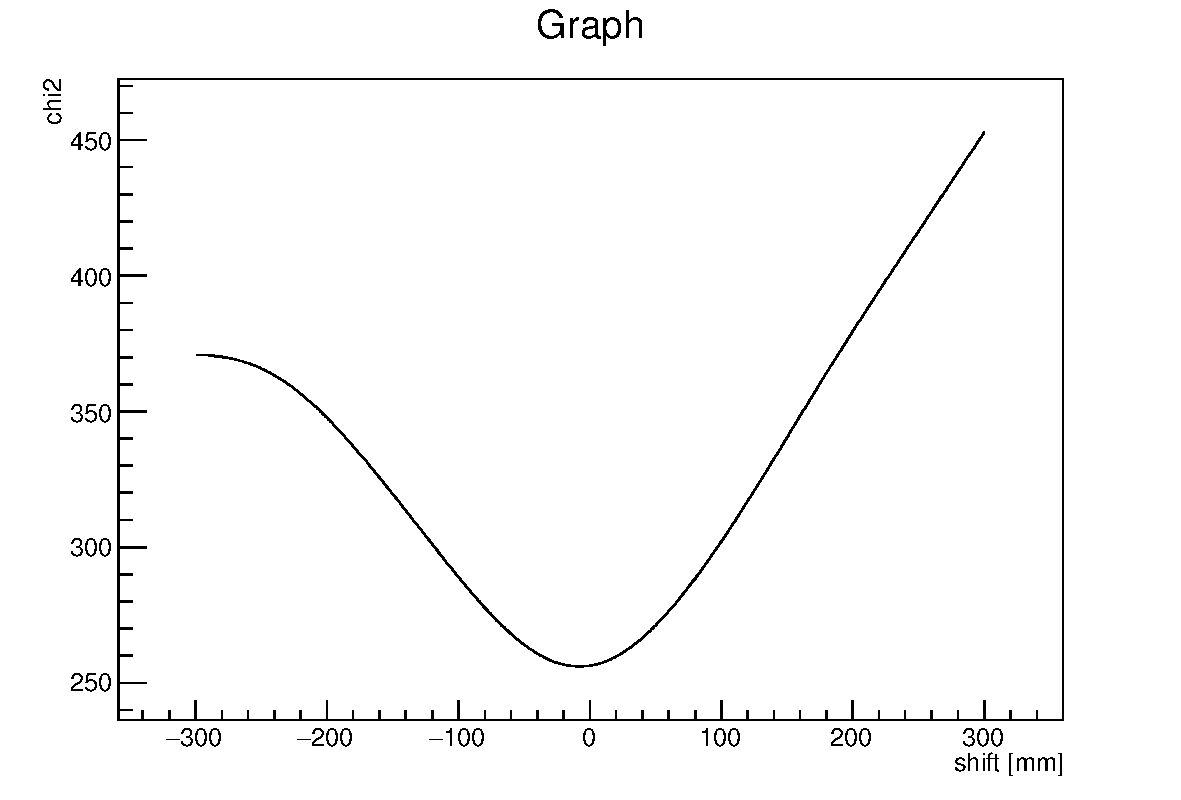
\includegraphics[width=0.33\textwidth]{./Figure/2017-08-02_Distribution_Chi2_1e8_LC.pdf}}
%   \subfloat[\label{fig:fig_Results_Chi2_Distribution_Variation_CC_simulation_Hadronth_LC}]{\includegraphics[width=0.33\textwidth]{./Figure/chi2_linecone.png}}
%  %\subfloat[\label{fig:fig_Results_Chi2_Distribution_Variation_CC_simulation_Hadronth_MLEM}]{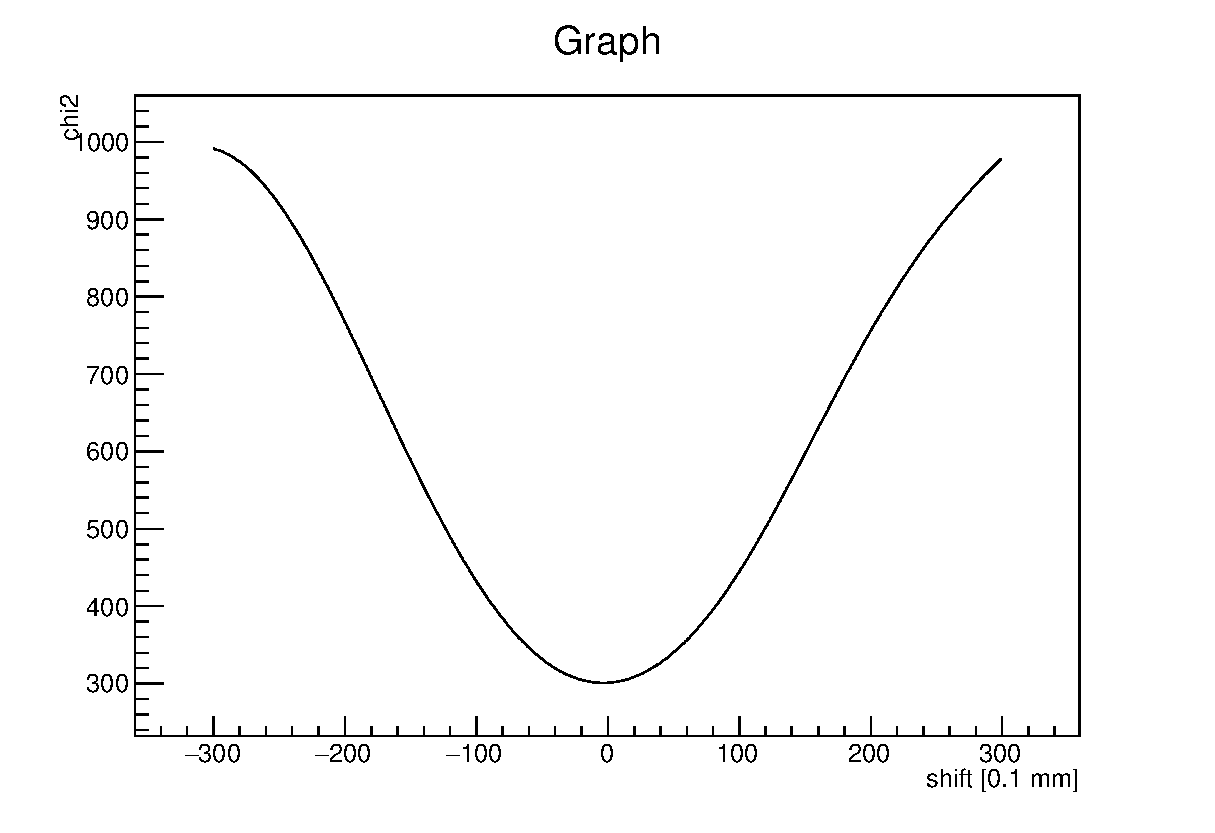
\includegraphics[width=0.33\textwidth]{./Figure/2017-08-02_Distribution_Chi2_Results_binning_1mm_ShiftNurbs0_1mm_1e8_article_MLEM.eps}}\\
%  \subfloat[\label{fig:fig_Results_Chi2_Distribution_Variation_CC_simulation_Hadronth_MLEM}]{\includegraphics[width=0.33\textwidth]{./Figure/chi2_MLEM.png}}\\
%   %\subfloat[\label{fig:fig_Results_Precision_Distribution_Variation_CC_simulation_Hadronth_LC} ]{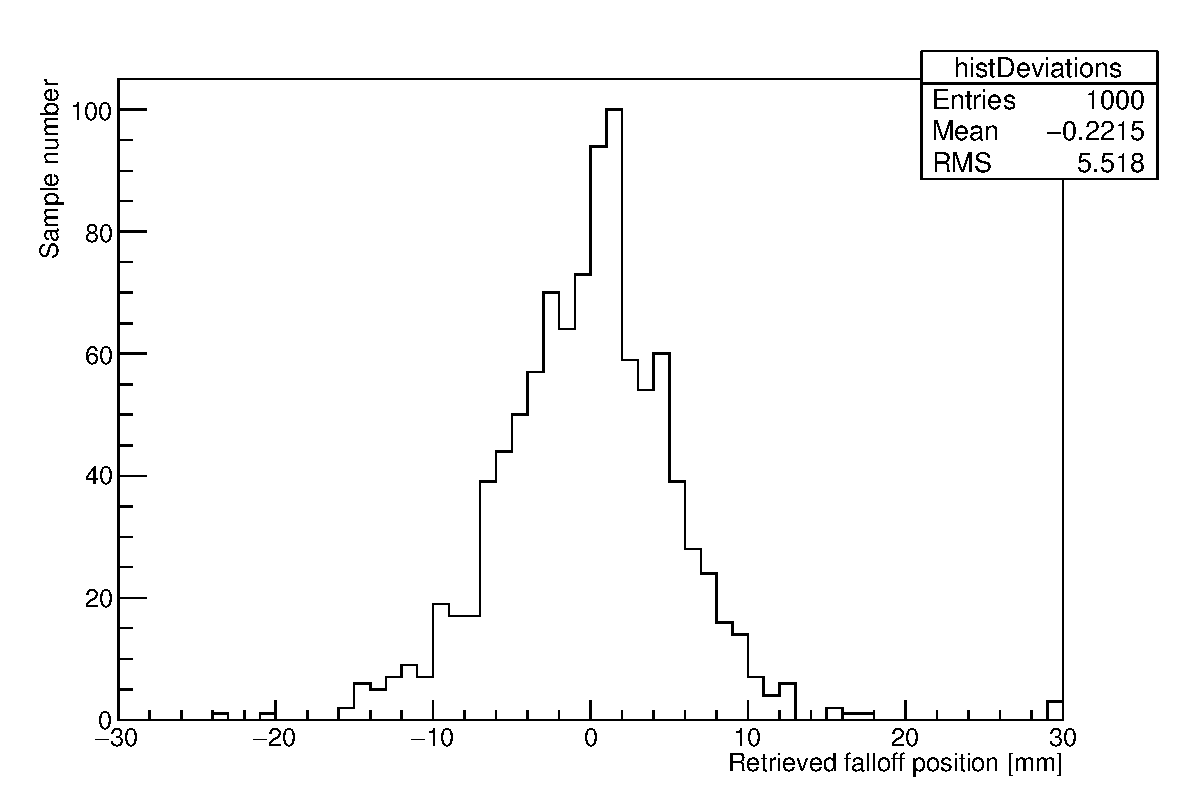
\includegraphics[width=0.33\textwidth]{./Figure/2017-08-02_Distribution_finale_1e8_Article_LC.pdf}}
%   \subfloat[\label{fig:fig_Results_Precision_Distribution_Variation_CC_simulation_Hadronth_LC} ]{\includegraphics[width=0.33\textwidth]{./Figure/deviation_linecone.png}}
%  %\subfloat[\label{fig:fig_Results_Precision_Distribution_Variation_CC_simulation_Hadronth_MLEM} ]{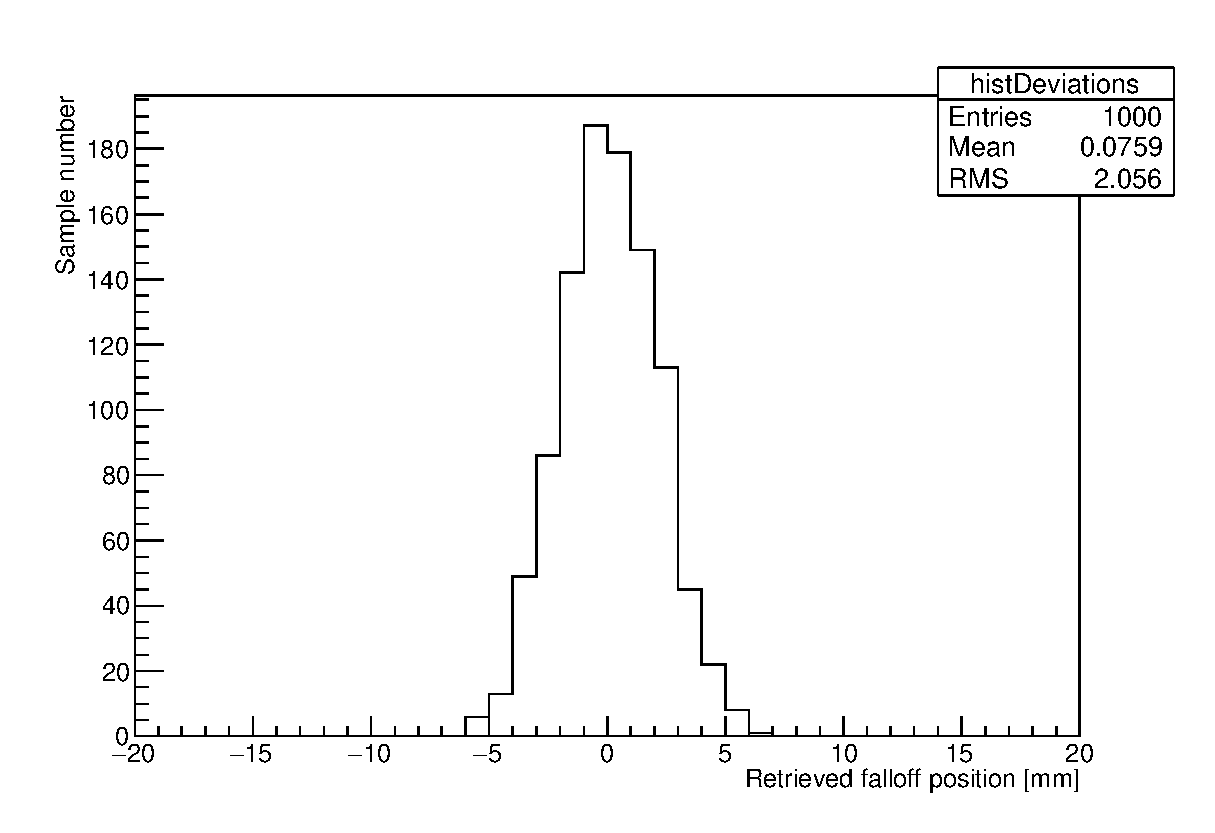
\includegraphics[width=0.33\textwidth]{./Figure/2017-08-02_FallOff_Results_binning_1mm_ShiftNurbs0_1mm_1e8_Article_MLEM.eps}}
%  \subfloat[\label{fig:fig_Results_Precision_Distribution_Variation_CC_simulation_Hadronth_MLEM} ]{\includegraphics[width=0.33\textwidth]{./Figure/deviation_MLEM.png}}
% \caption{Data processing comparison for the same proton simulation with the line cone algorithm (left column) and the LM-MLEM algorithm (right column). The first row gives the reconstructed profile for $10^{10}$ incident protons. The second row shows the reference curve (blue) and the curve obtained with a $10^8$ incident protons subset. The third row shows the $\chi^2$ distribution for one data subset. The last row represents the distribution of the minimal calculated shifts for 1000 subsets at the same statistics of $10^8$ incident protons.}
% \end{figure}

\section{Results}

The possible implementation of the CLaRyS Compton camera as a monitoring system for ion beam therapy has been investigated. The detection efficiency of the camera has been estimated with point-like gamma sources set in different positions with respect to the center of the camera. A PMMA cylindrical phantom has been simulated and exposed to proton and carbon beams at increasing intensities for an analysis of the prompt gamma detection environment (background, random coincidence contamination). The camera precision in the identification of the fall-off of the prompt gamma emission profile has been investigated. For this purpose, the comparison of two different reconstruction methods (line-cone analytical reconstruction and MLEM iterative algorithm) is presented. In the following sections we show the obtained results. 


\subsection{Absolute detection efficiency}
\label{Results::efficiency}

Figure~\ref{fig::efficiency_study} shows the absolute gamma detection efficiency as a function of the gamma source position with respect to the center of the camera in the transverse plane. On the left side, we show the results achieved with an ideal detector. On the right side realistic energy cuts are applied on each detector section: the lower energy limit has been set to 50~keV for the scatterer and 100~keV for the absorber. 

\begin{figure} [!hbtp]	
\centering
%\subfloat[]{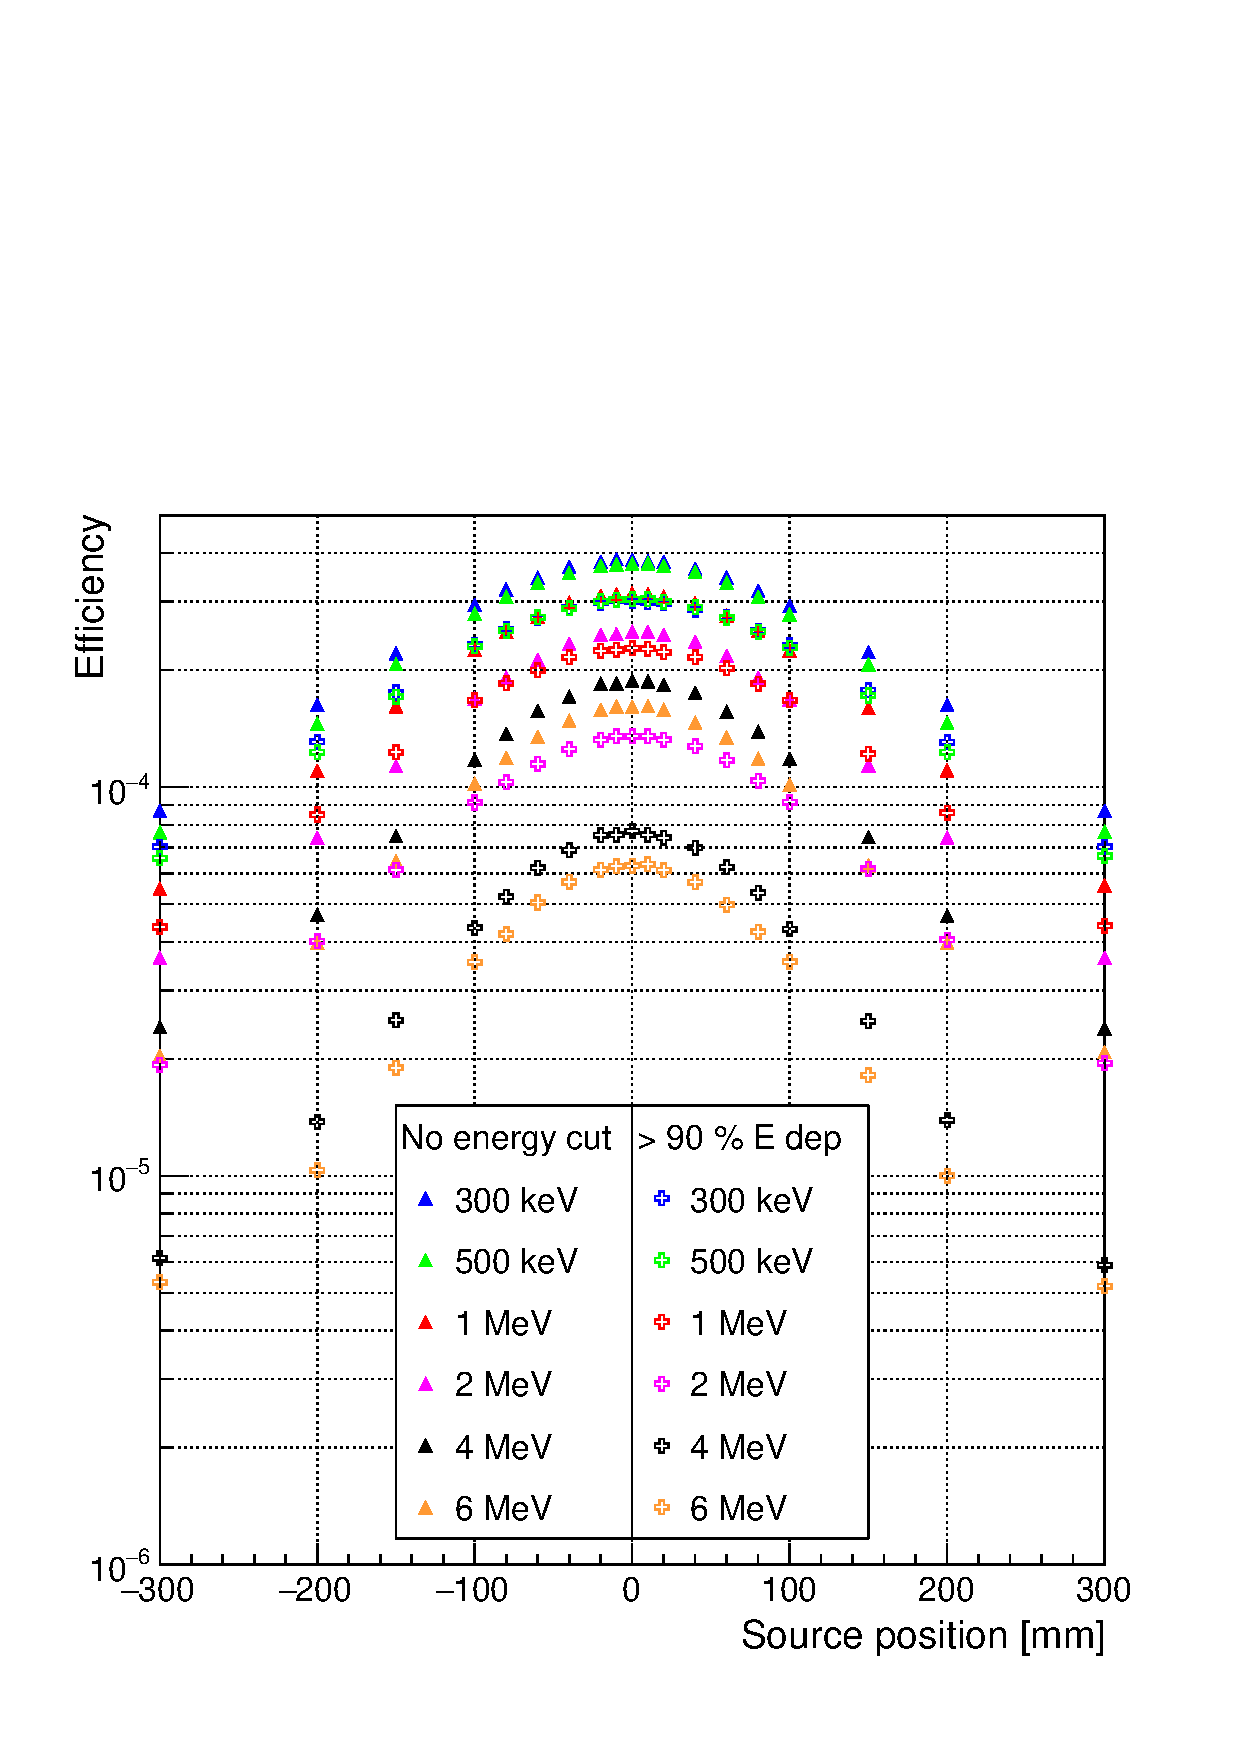
\includegraphics[width=0.5\textwidth]{./Figure/new/EffVSpos_withSumCut.pdf}}
\subfloat[]{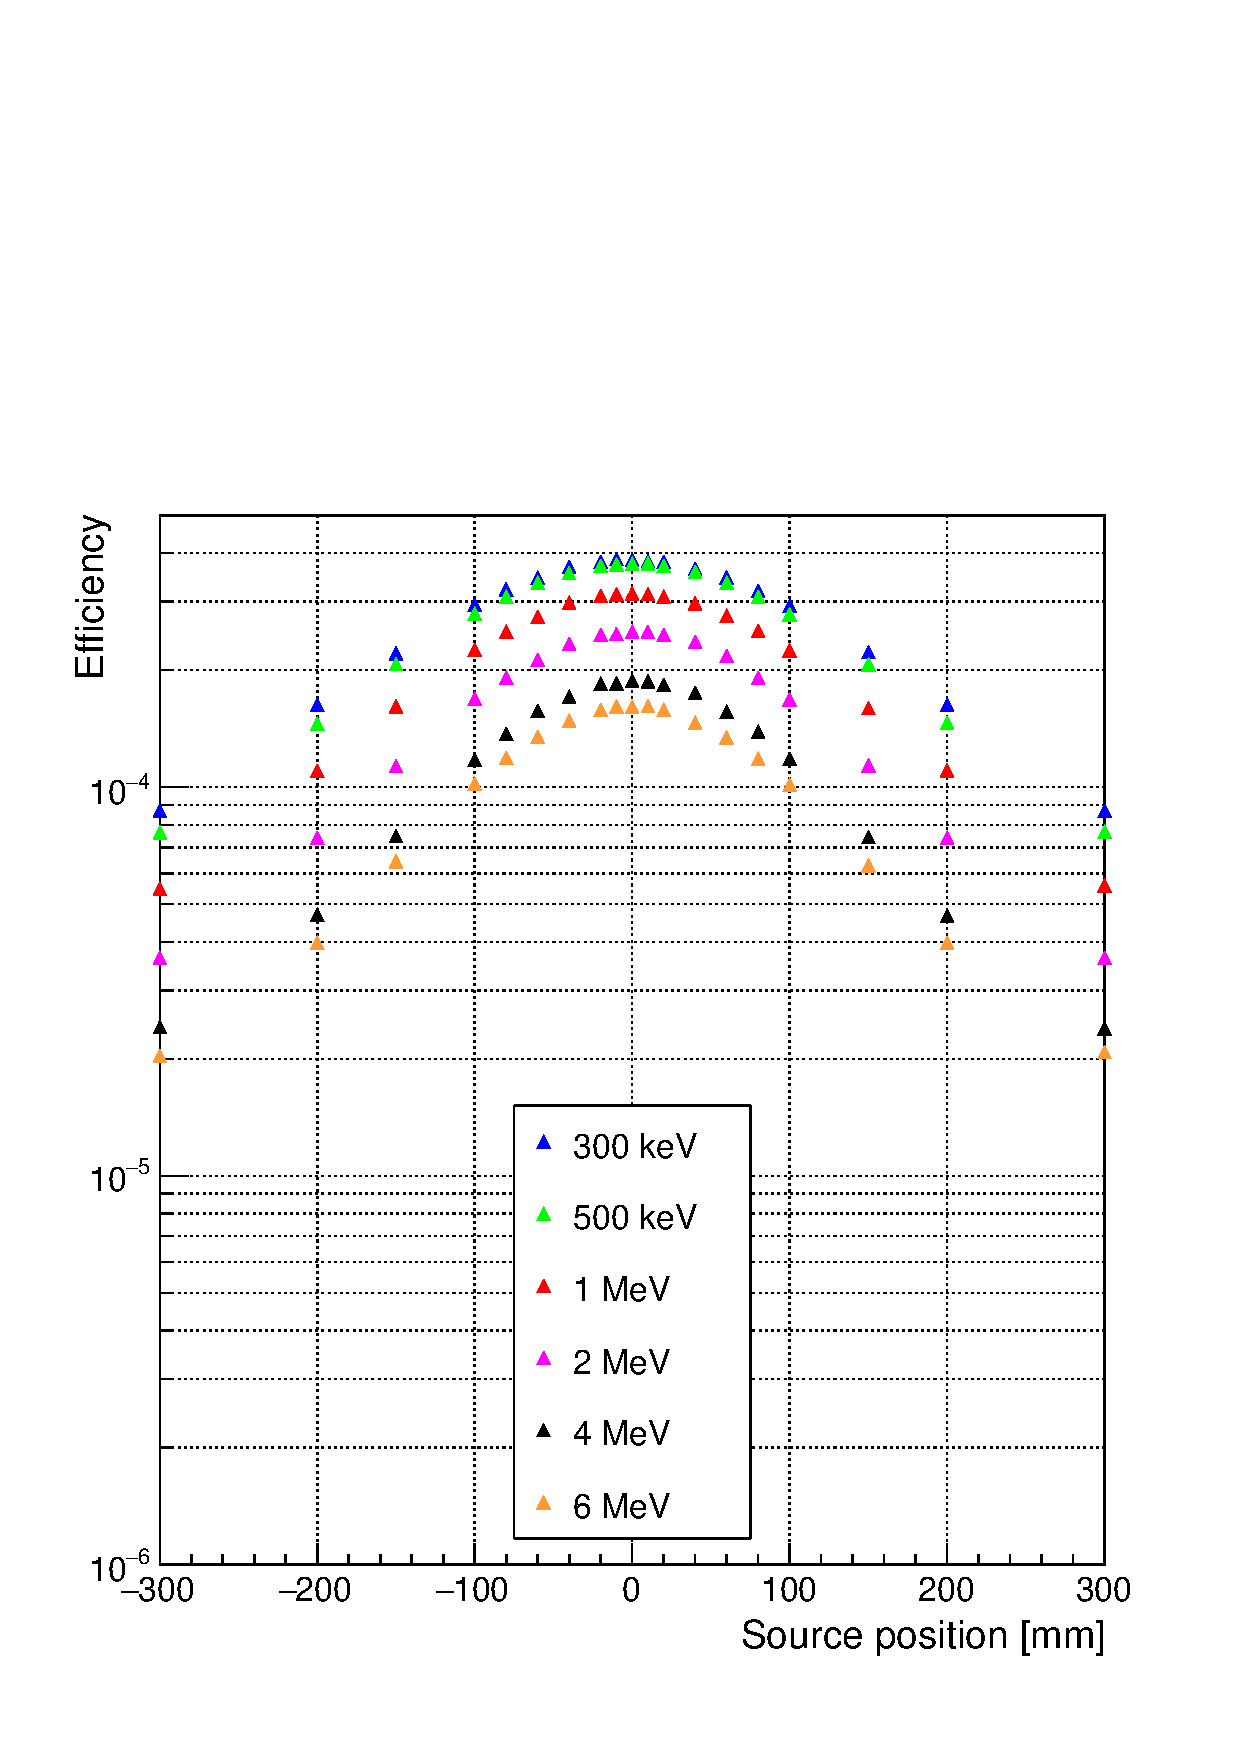
\includegraphics[width=0.5\textwidth]{03_GraphicFiles/chapter3/HT/new/EffVSpos_noCut_simple.pdf}}
%\subfloat[]{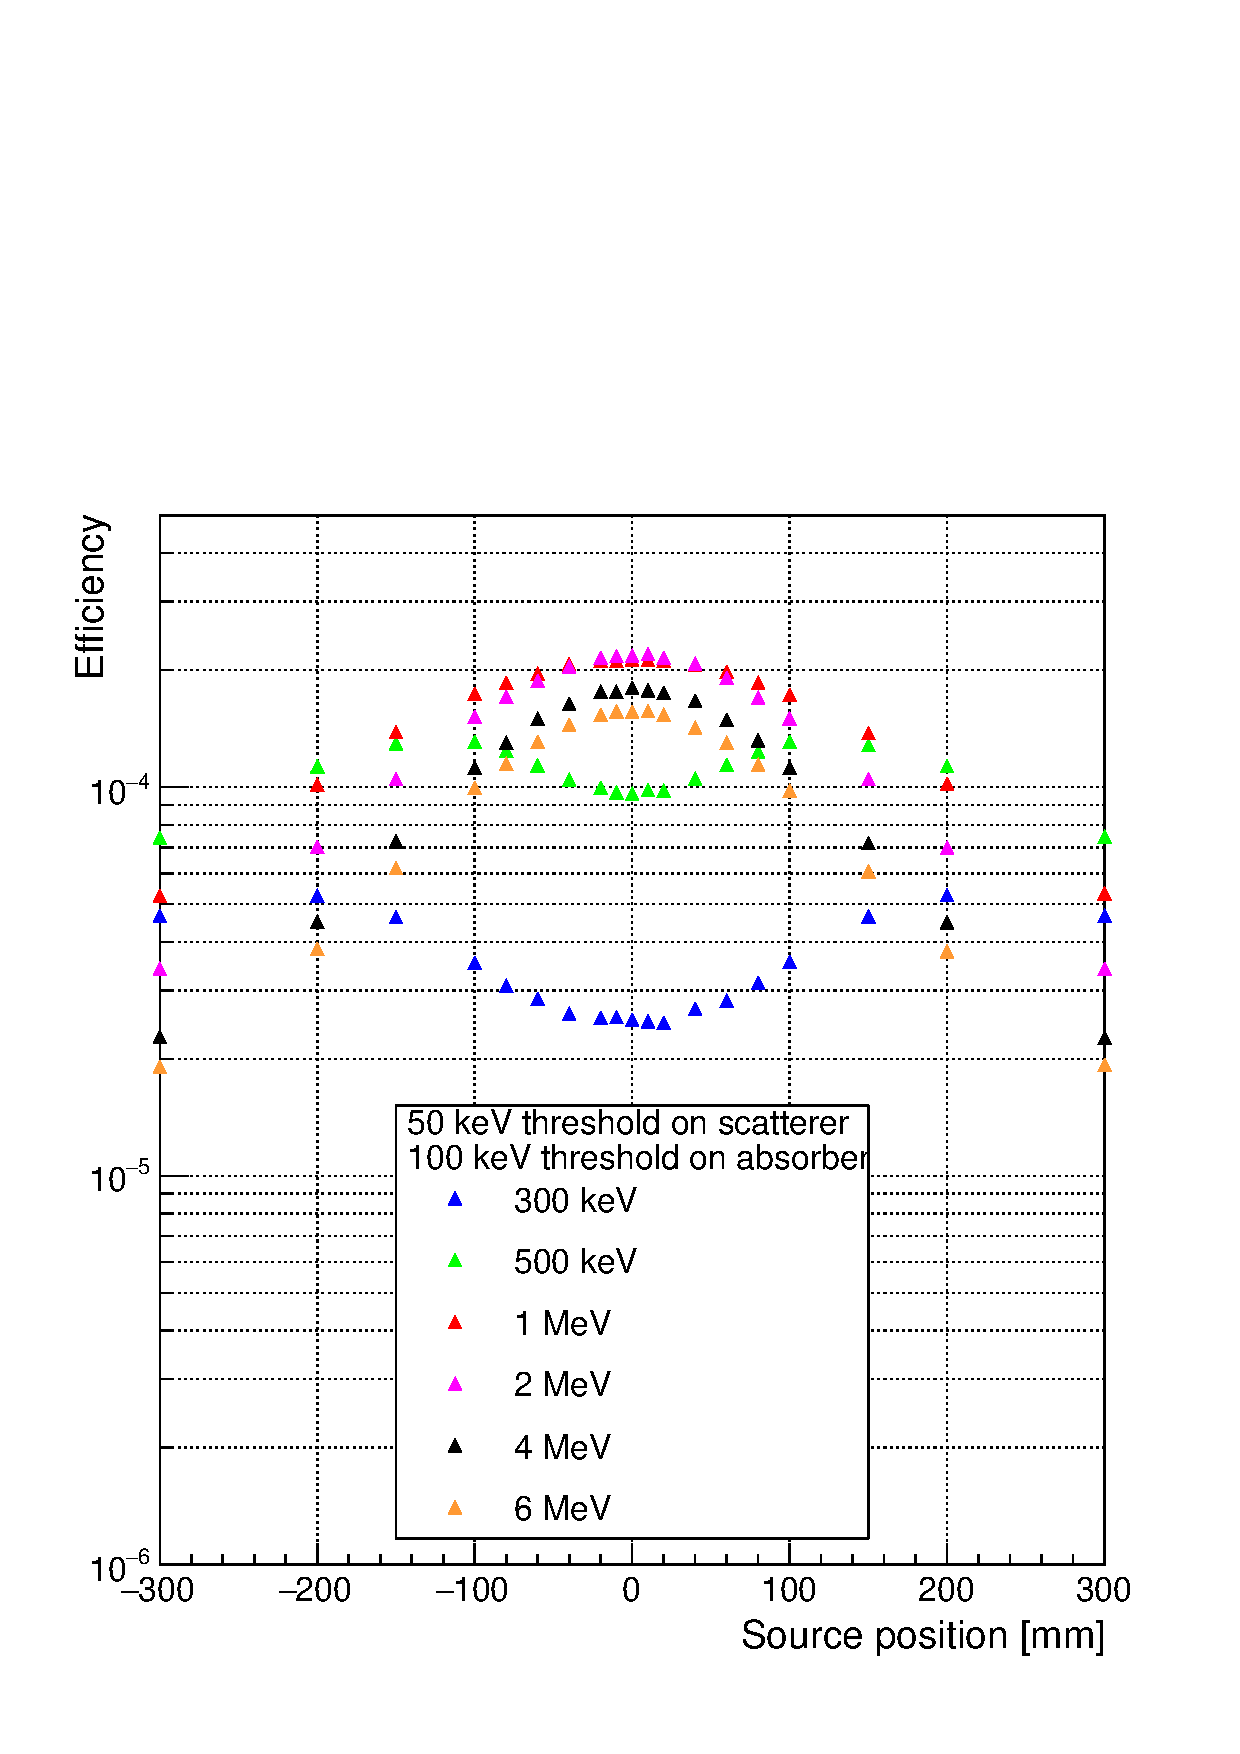
\includegraphics[width=0.5\textwidth]{./Figure/new/EffVSpos_withSingleCut.pdf}}
\subfloat[]{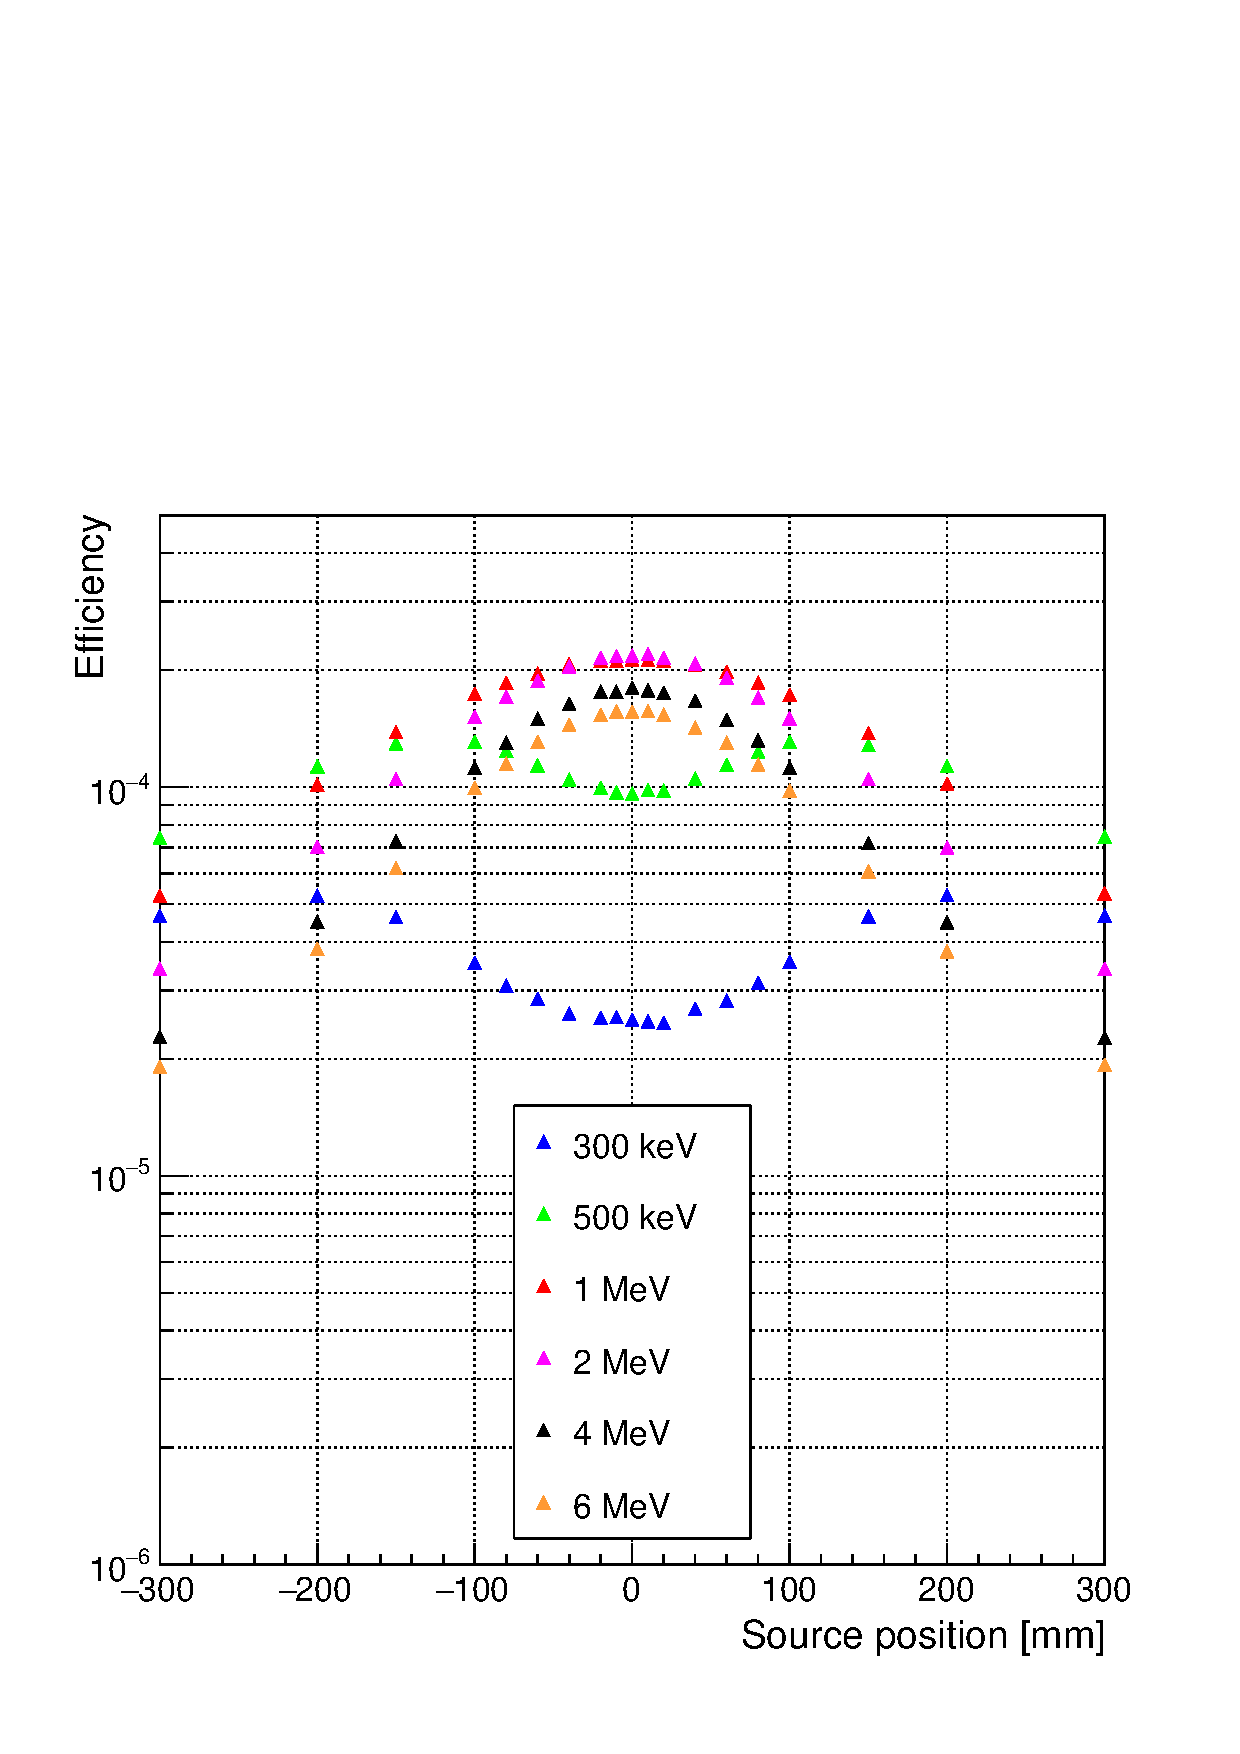
\includegraphics[width=0.5\textwidth]{03_GraphicFiles/chapter3/HT/new/EffVSpos_CutSingle_simple.pdf}}
\caption{Absolute Compton camera efficiency as a function of the gamma source position for different gamma energies, in the range between 300~keV to 6~MeV. The left side shows the camera efficiency with no data selection. In the right side, detection energy thresholds are applied: the lower energy thresholds are set to 
50~keV for the scatterer and 100~keV for the absorber, to reproduce a realistic scenario. These values can change for the final configuration, according to the detector energy resolutions achieved.}
\label{fig::efficiency_study}
\end{figure}

As expected according to the interaction probability energy dependency, the efficiency is higher for low gamma energies, and it lies in the range $4\times10^{-4}$ at 300~keV and $1.5\times10^{-4}$ at 6~MeV at the center of the camera. Moreover, it can be noticed how the efficiency slightly drops as the point source is shifted away from the camera center: efficiency reductions at 500~keV and 4~MeV are respectively of 25\% and 35\%. This effect is more important for high energies, for which the incident gamma is less deflected in the scatterer for the same energy deposited compared to a low energy gamma (see equation~\ref{Compton_equation}).\\  
Figure~\ref{fig::efficiency_study}(b) shows the effect of realistic camera detection thresholds as opposed to ideal detection. The gamma detection efficiency drops of a factor ranging from about 1.25 to more than an order of magnitude for the central detection area for energies in the range 300~keV - 2~MeV respectively. The effect is reduced by the distance of the source from the center of the camera. Negligible effects are detected for positions with a distance greater than 200~mm from the center of the camera, and for any distance at energies above 2~MeV, while the efficiency is reduced in the central area of the camera.\\

\begin{figure} [!hbtp]	
\centering
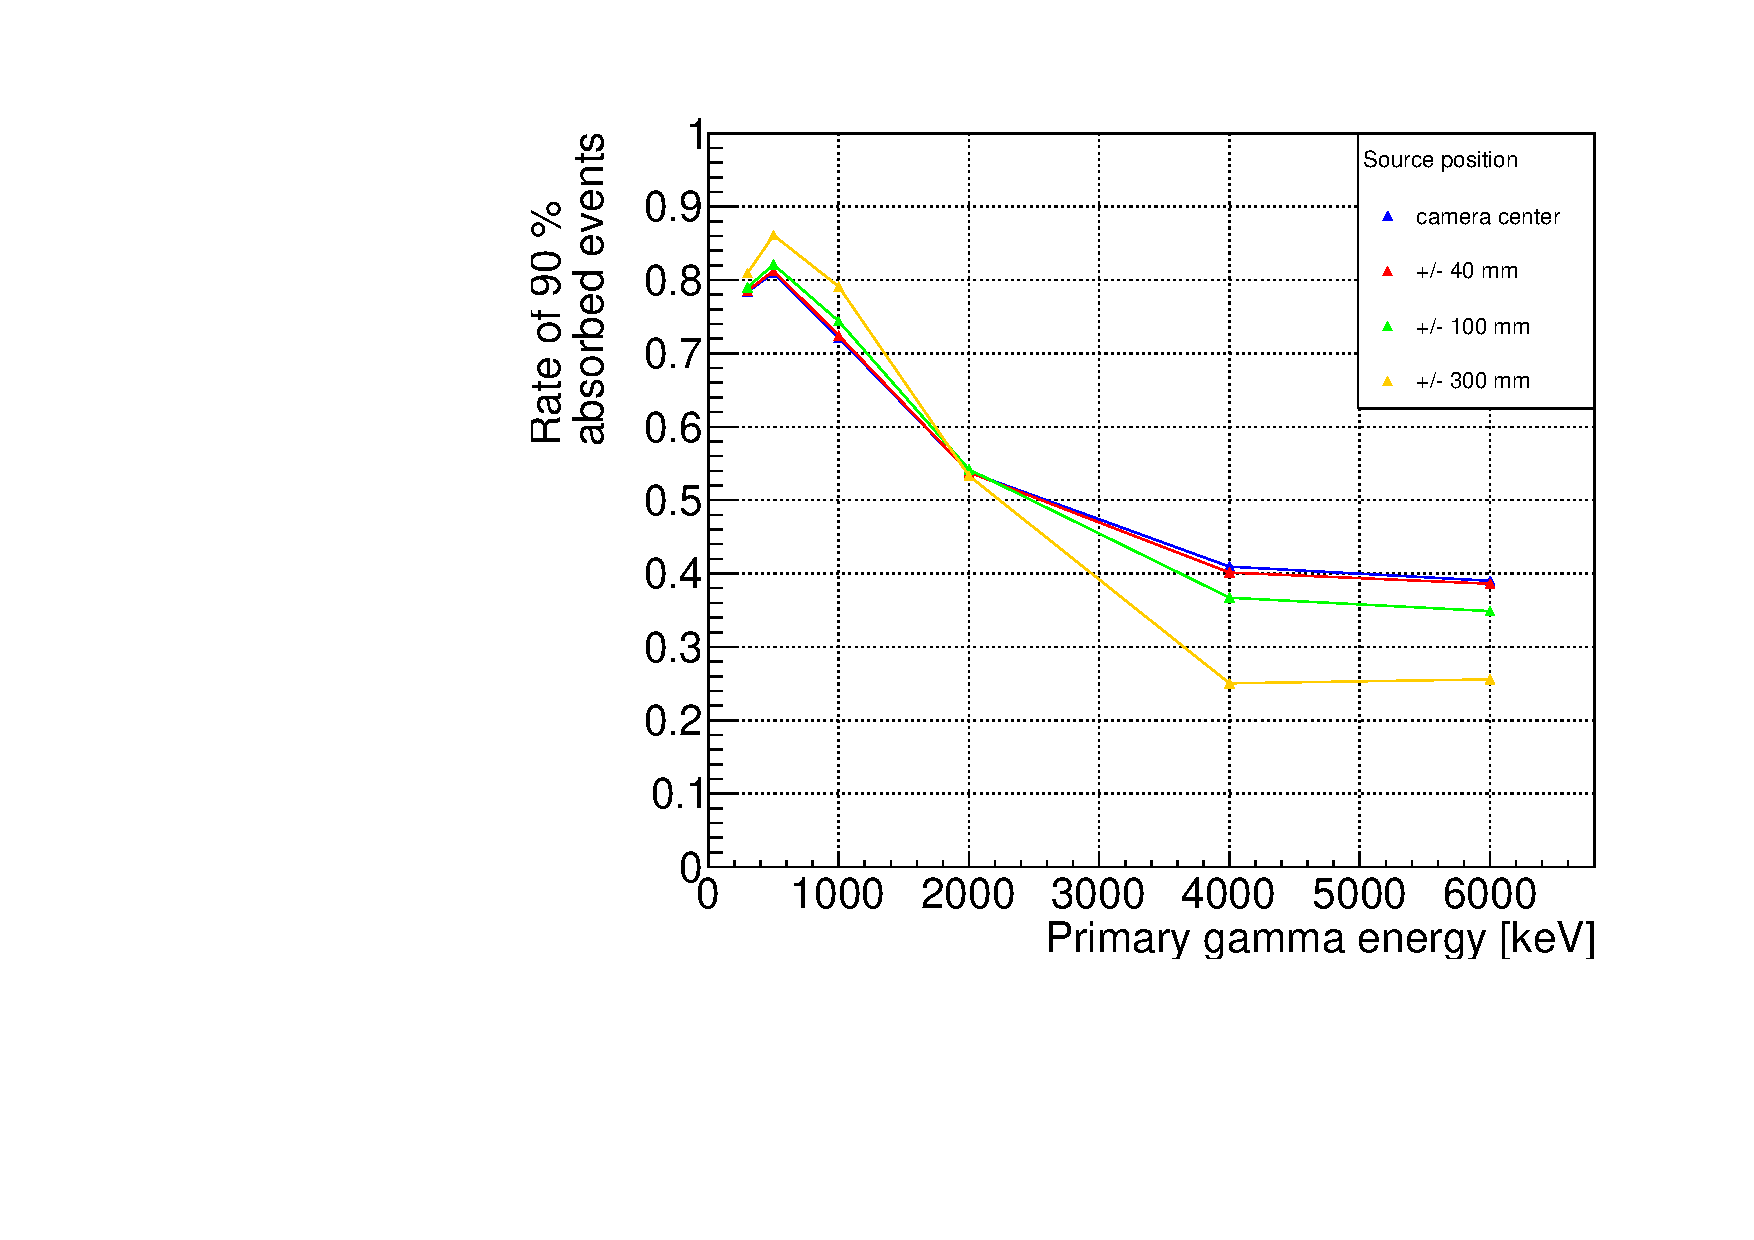
\includegraphics[width=0.5\textwidth]{03_GraphicFiles/chapter3/HT/new/rate_90percent_energy_4distances.pdf}
\caption{Ratio between coincidence events with more than 90\% of the primary photon energy absorbed in the detector layer and all detected coincidences for 4 source positions: center of the camera, 40, 100, 300~mm from the center.}
\label{fig::rate_full_abs}
\end{figure}


Figure~\ref{fig::rate_full_abs} shows the rate of events with more than 90\% of the primary gamma energy deposited in the detector layers, for 4 different source positions (center of the camera, 40, 100, 300~mm far from the center) with no selection applied on a single detector layer basis. As expected, the rate of almost fully absorbed events decreases as the energy increases, in a range between more than 80\% and 40\% for 300~keV and 6~MeV primary photon energy, respectively, with the source at the center of the camera. Also the source position has an impact, with a 35\% reduction if moving from the center to a distance of 300~mm in the transverse plane. For lower energies, the rate of fully absorbed events slightly increases when the source is moving away from the camera center, with maximum variations of less than 10\%. 
 

\subsection{Rate of random coincidences}
\label{Results::beamInt}
 
In figure~\ref{fig:coincidences}, the different components of the signal resulting from the PMMA exposure to proton and carbon ion beams are shown as a function of the beam intensity. The true coincidences represent scatterer-absorber time coincidences generated by the same gamma ray. All the other coincidence types compose the background. The collected data sets are reported with and without the applied time-of-flight discrimination, mainly employed for neutron rejection, as mentioned in section~\ref{MatMeth::TOF_Ecut}.


\begin{figure} [!h]
  %\subfloat[]{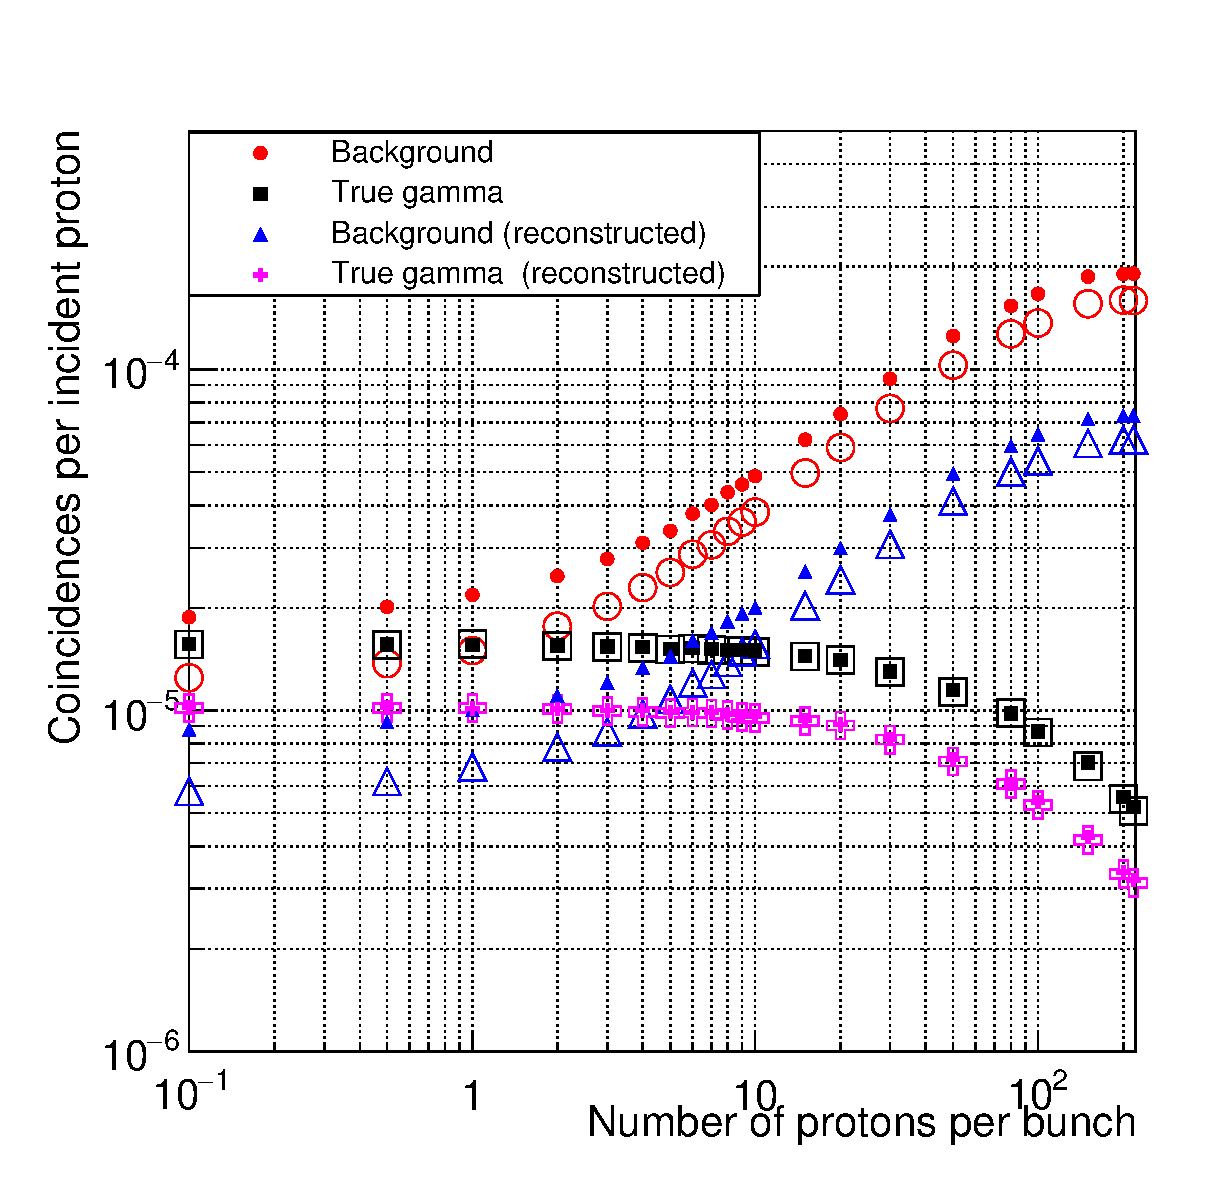
\includegraphics[width=0.5\textwidth]{./Figure/2017_06_28_Taux_coincidences_variation_protons_New_design_4EntreesLegend_LogXLogY.eps}}
  \subfloat[]{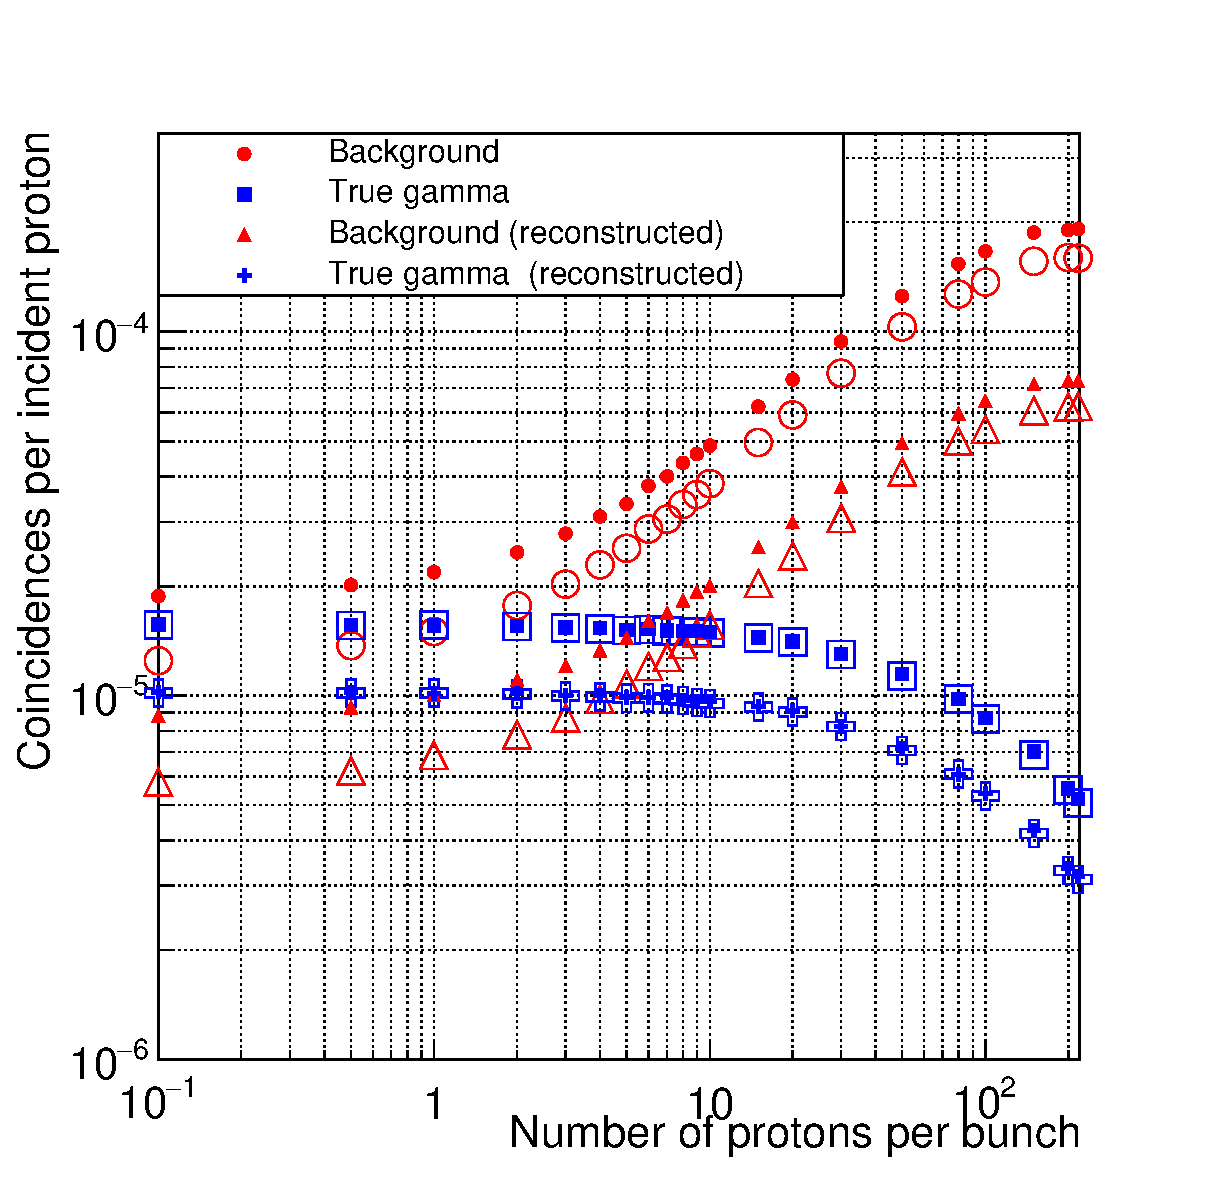
\includegraphics[width=0.5\textwidth]{03_GraphicFiles/chapter3/HT/new/coincYields_protons.eps}}
  %\subfloat[]{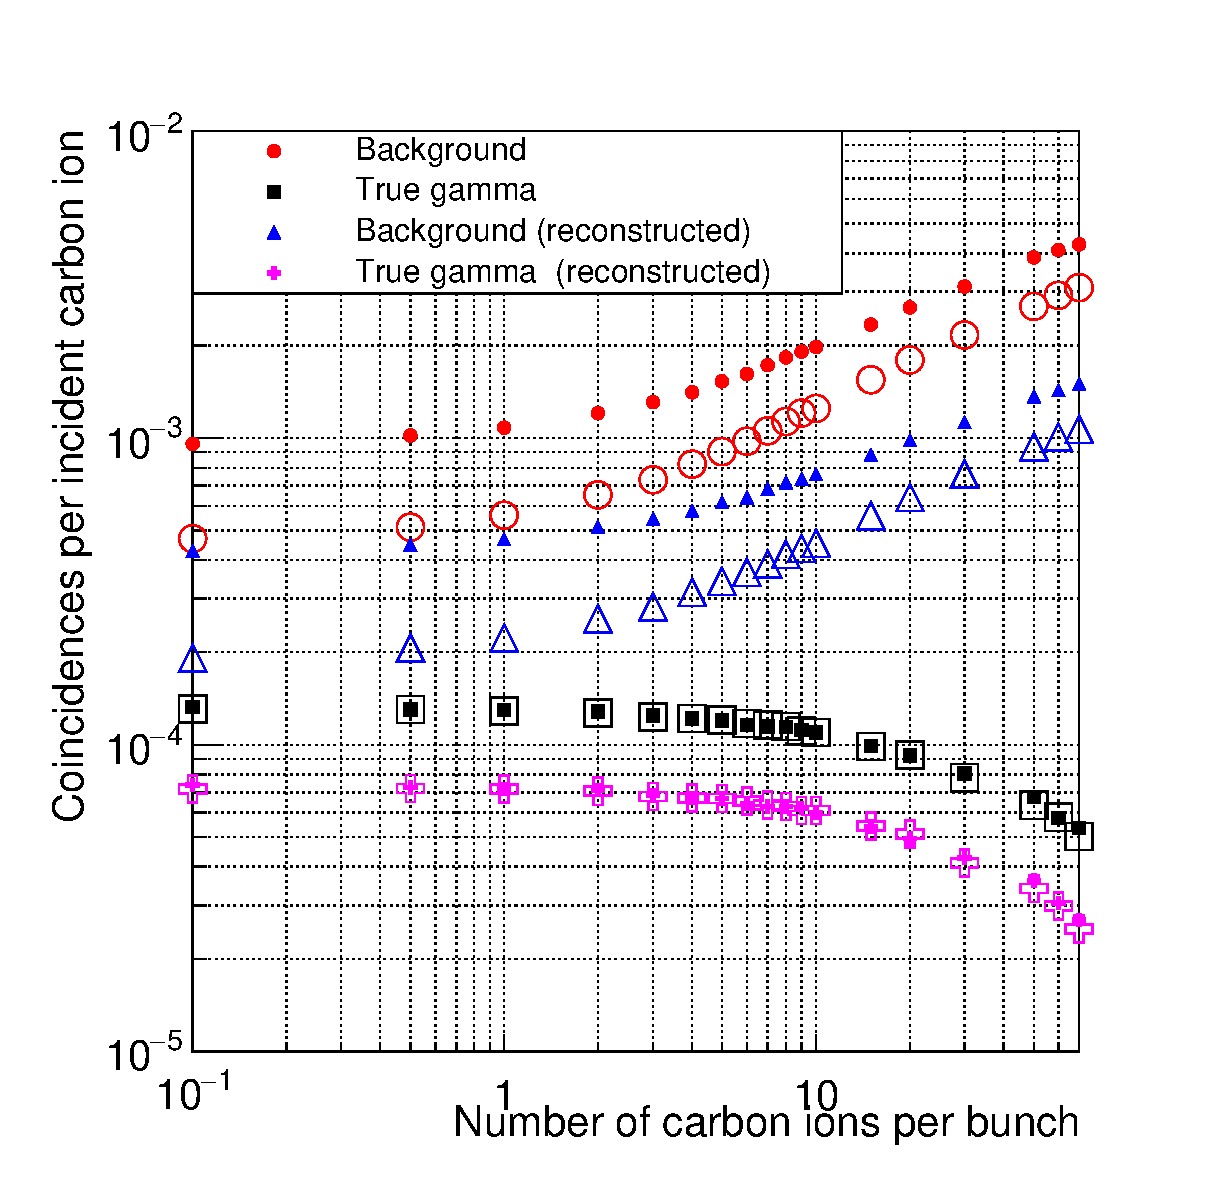
\includegraphics[width=0.5\textwidth]{./Figure/2017_06_28_Taux_coincidences_variation_carbonIons_New_design_4EntreesLegend_LogXLogY.eps}}
  \subfloat[]{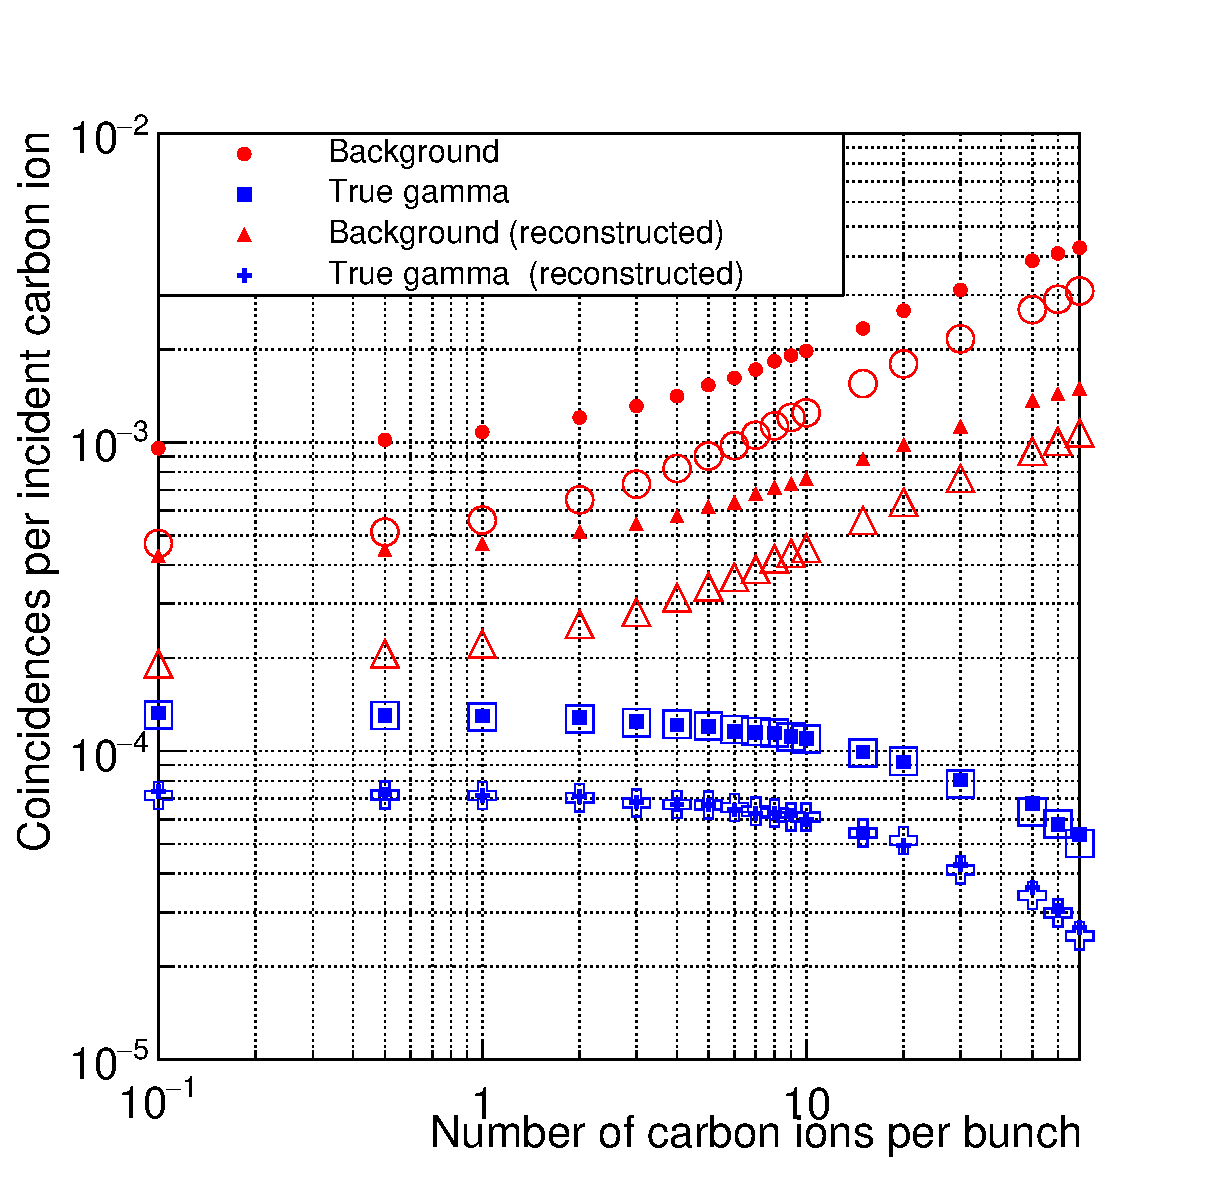
\includegraphics[width=0.5\textwidth]{03_GraphicFiles/chapter3/HT/new/coincYields_Cions.eps}}
  \caption{Coincidences yield for protons (left) and carbon ions (right) as a function of the beam intensity. The intensity is reported as number of incident particles per bunch. The filled markers correspond to the collected data without time-of-flight discrimination, while this cut is applied to the data reported with empty markers. Moreover, the yields are given before and after the profile reconstruction with the line-cone algorithm.}
  \label{fig:coincidences}
\end{figure}

In figure~\ref{fig:coincidences}(a) and (b) the amount of true gamma coincidences and background events are reported before and after reconstruction via line-cone algorithm as a function of the beam intensity for proton (a) and carbon ion (b) beams. In addition to this, for each curve realized with the complete collected data set, the related one realized after time-of-flight selection of events is sketched (empty symbols). All the curves have been normalized to the number of incident ions.

The amount of background events (mainly random coincidences) increases with the increasing beam intensity: a factor of about 30 with respect to true gamma events is obtained for proton beams at  the intensity of 200 protons per bunch with no event selection, while a factor more than two times higher is reported for carbon ions in the same conditions. The time-of-flight selection can slightly improve the signal -over-noise ratio by reducing the amount of background events. The amount of true gamma events and background events becomes similar at the intensity of about 1 proton per bunch.


\subsection{Camera precision}
\label{Results::precision_reconstruction}
Given the results presented in the previous section, the camera precision in the fall-off identification is investigated with proton beams at reduced intensities.
%The simulation setup shown in figure~\ref{fig:fig_setup_CC_simulation_Hadronth} has been implemented to test the line-cone analytic reconstruction method and compare it to the iterative LM-MLEM algorithm~\cite{maxim_filtered_2014,hilaire_compton_2014}. 
A single data set has been collected, corresponding to the irradiation of the PMMA phantom with a proton 160~MeV monoenergetic beam, with a reduced intensity of 1 proton per bunch. A total of $10^{10}$ protons has been simulated to define the reference PG profile, and then different low statistics profiles have been produced for the precision estimate as explained in section~\ref{MatMeth:precision}. 

The high statistics profile reconstructed via line-cone algorithm is shown in figure~\ref{fig:fig_Results_Estimation_Camera_Profil_highStat_CC_simulation_Hadronth_LineCone} and via the LM-MLEM reconstruction method in figure~\ref{fig:fig_Results_Estimation_Camera_Profil_highStat_CC_simulation_Hadronth_MLEM}. A NURBS model of a low statistics sample ($10^8$ incident protons) is shown in figures~\ref{fig:fig_Estimation_Camera_CC_NURBS_Poisson_LC} for the line cone and~\ref{fig:fig_Estimation_Camera_CC_NURBS_Poisson_MLEM} for the MLEM.
Figures~\ref{fig:fig_Results_Chi2_Distribution_Variation_CC_simulation_Hadronth_LC} and~\ref{fig:fig_Results_Chi2_Distribution_Variation_CC_simulation_Hadronth_MLEM} show the distribution of $\chi^2$ calculated for a low statistic profile at $10^8$ incident protons. The retrieved optimal shift distribution is shown in figure~\ref{fig:fig_Results_Precision_Distribution_Variation_CC_simulation_Hadronth_LC} and~\ref{fig:fig_Results_Precision_Distribution_Variation_CC_simulation_Hadronth_MLEM} for the line-cone and LM-MLEM algorithm respectively, for $10^8$ incident protons as well.
Figure~\ref{fig:comparison} shows the results of the reconstruction of the profile obtained with 10$^8$ primary protons.


\begin{figure}
  \centering
  %\subfloat[\label{fig:fig_Results_Estimation_Camera_Profil_highStat_CC_simulation_Hadronth_LineCone}]{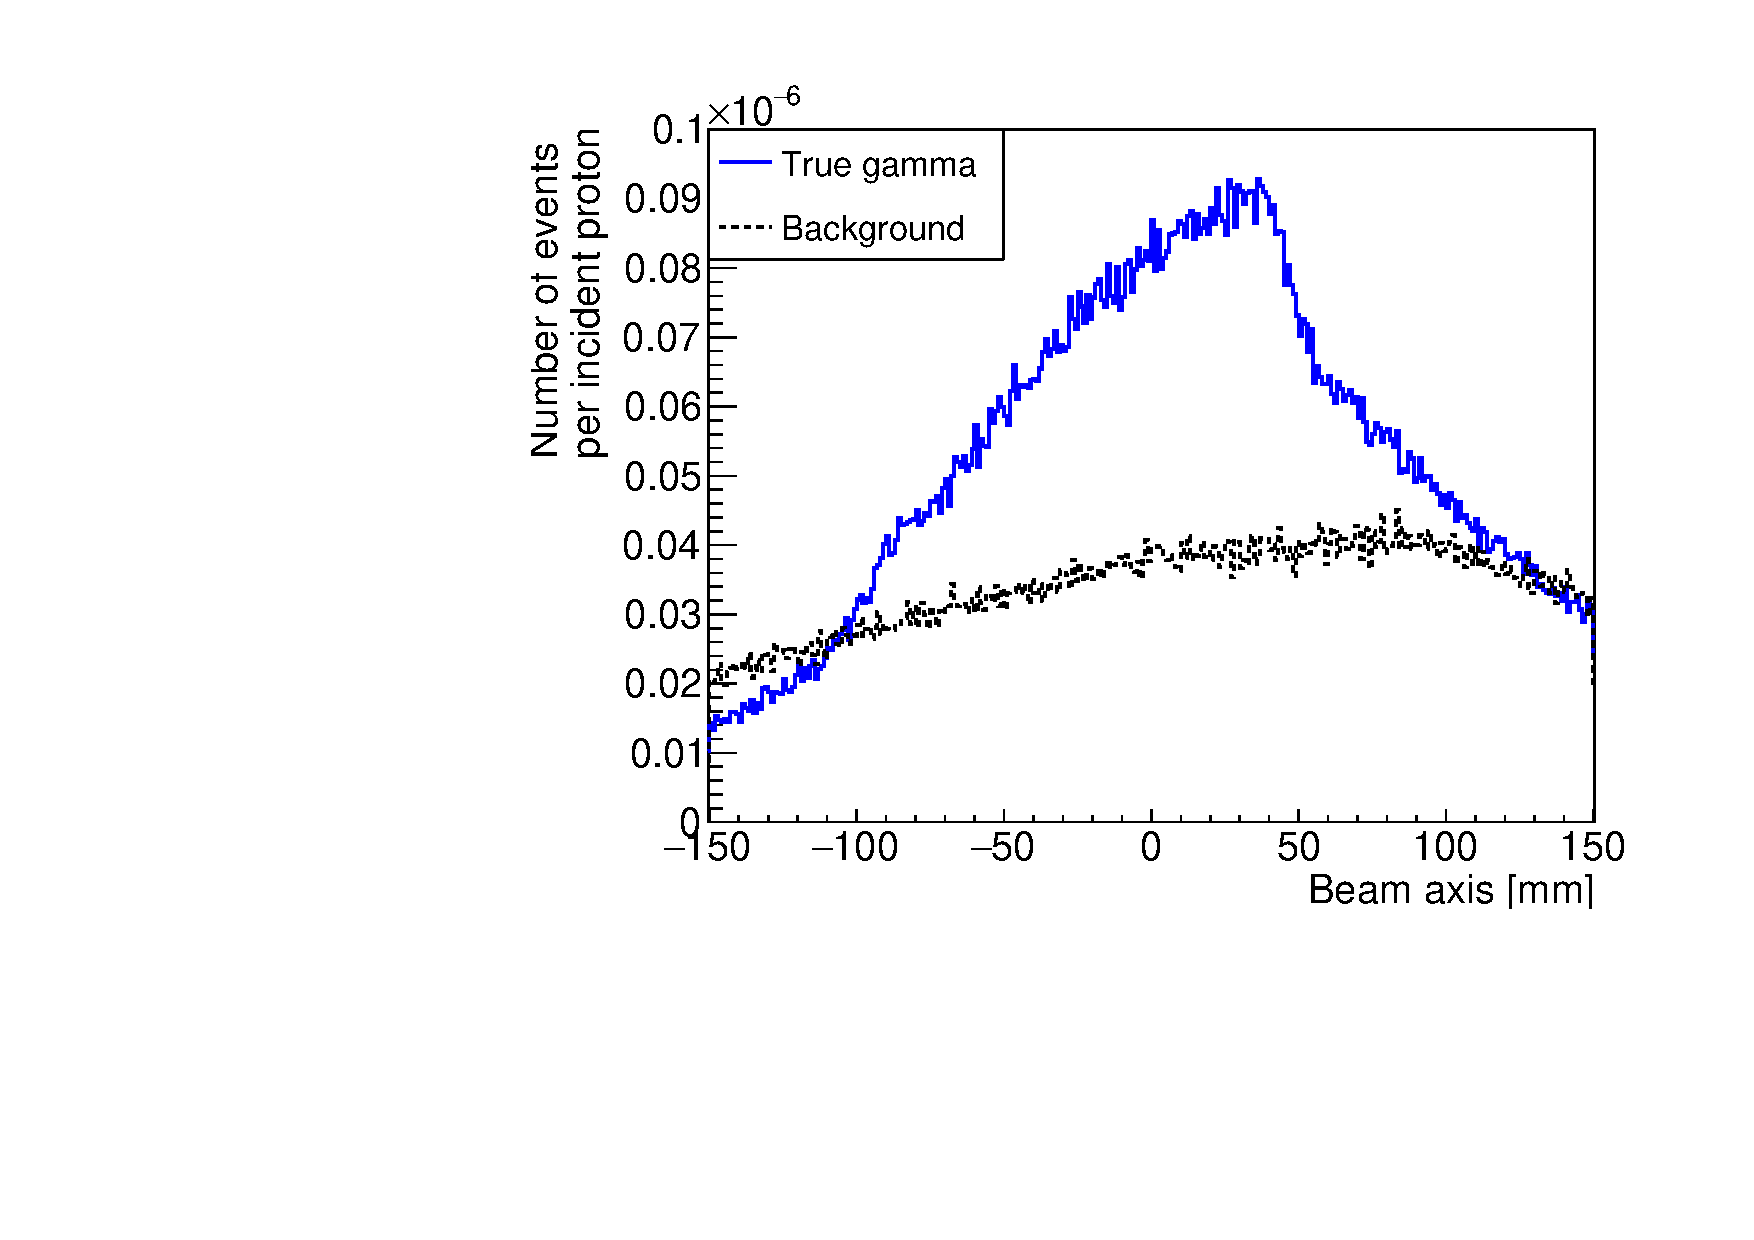
\includegraphics[width=0.48\textwidth]{./Figure/profile_high_stat_linecone_2.pdf}}
	\subfloat[\label{fig:fig_Results_Estimation_Camera_Profil_highStat_CC_simulation_Hadronth_LineCone}]{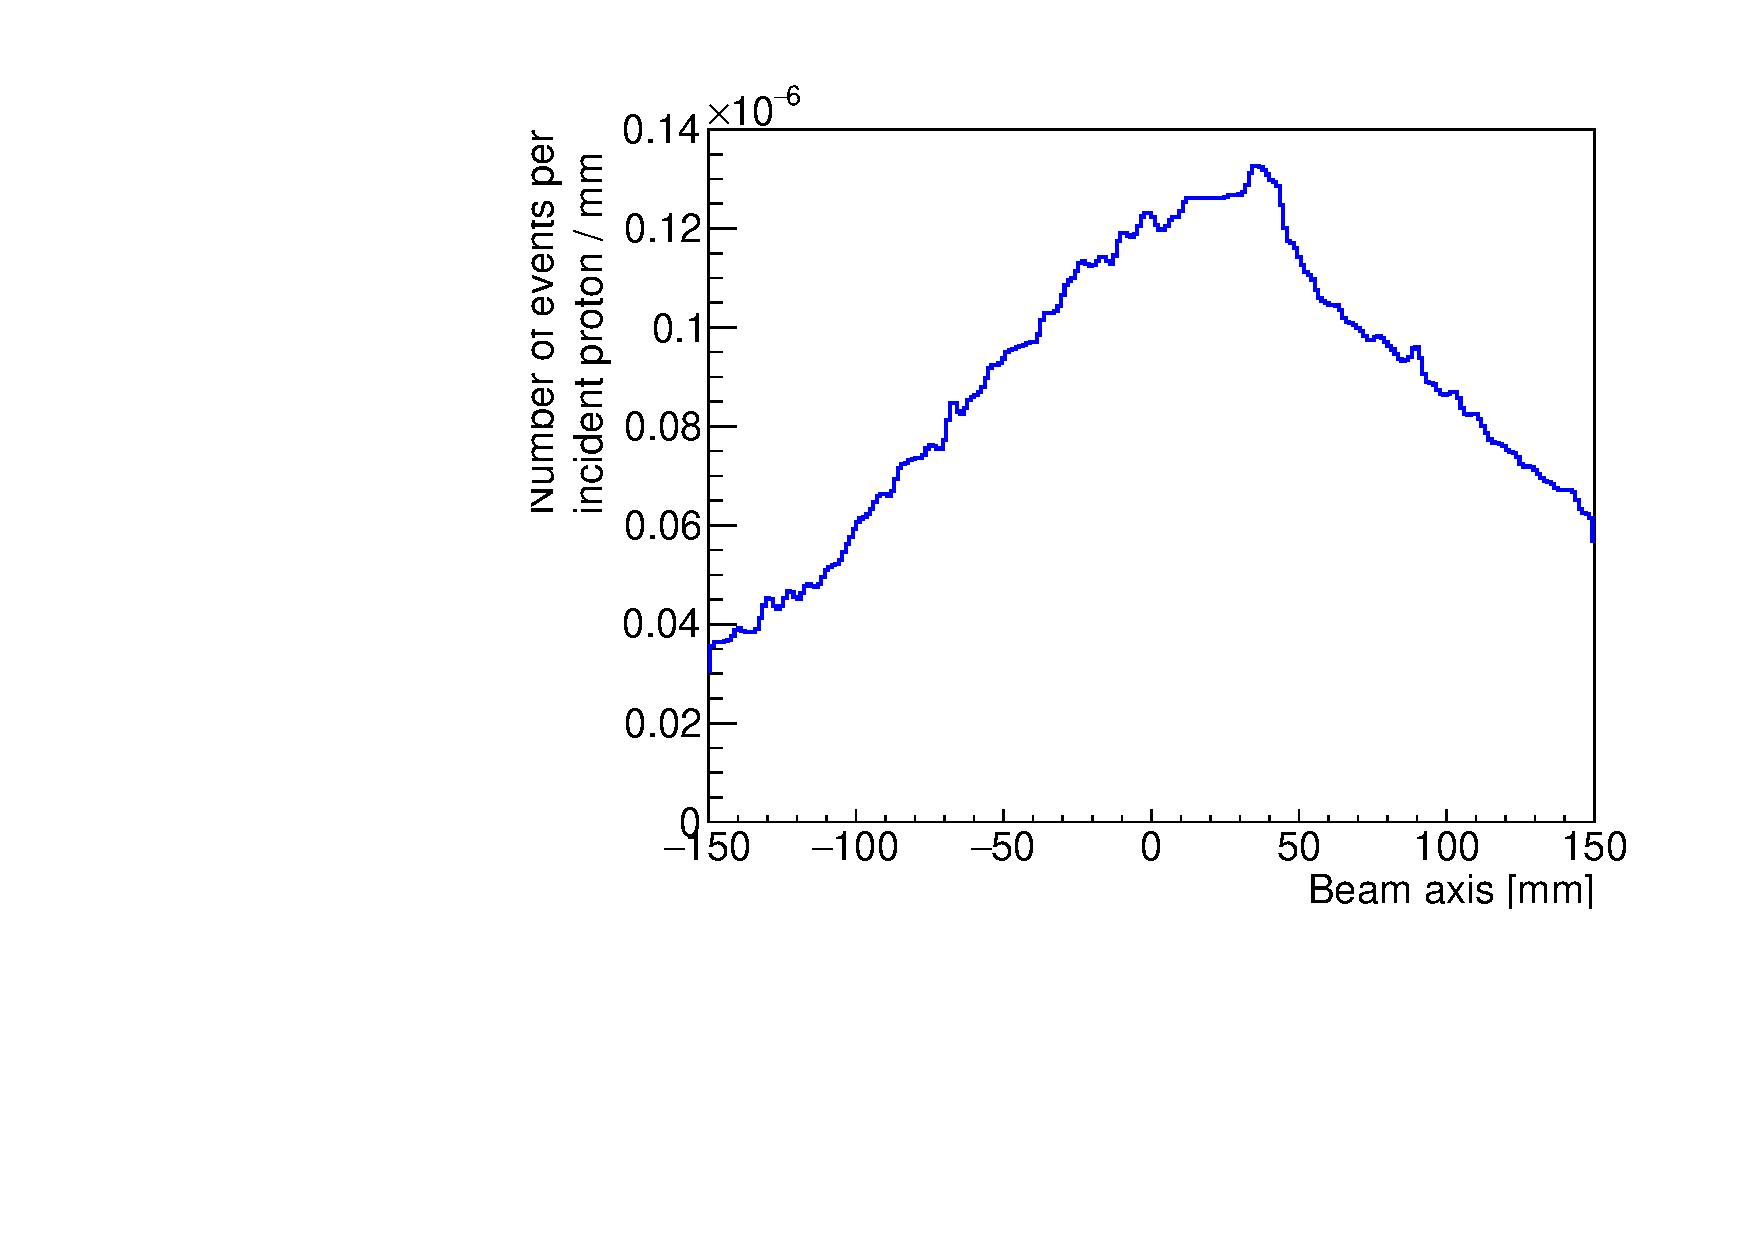
\includegraphics[width=0.48\textwidth]{03_GraphicFiles/chapter3/HT/new/reconstructed_histStat_profile_lineCone_norm.pdf}}
 % \subfloat[\label{fig:fig_Results_Estimation_Camera_Profil_highStat_CC_simulation_Hadronth_MLEM}]{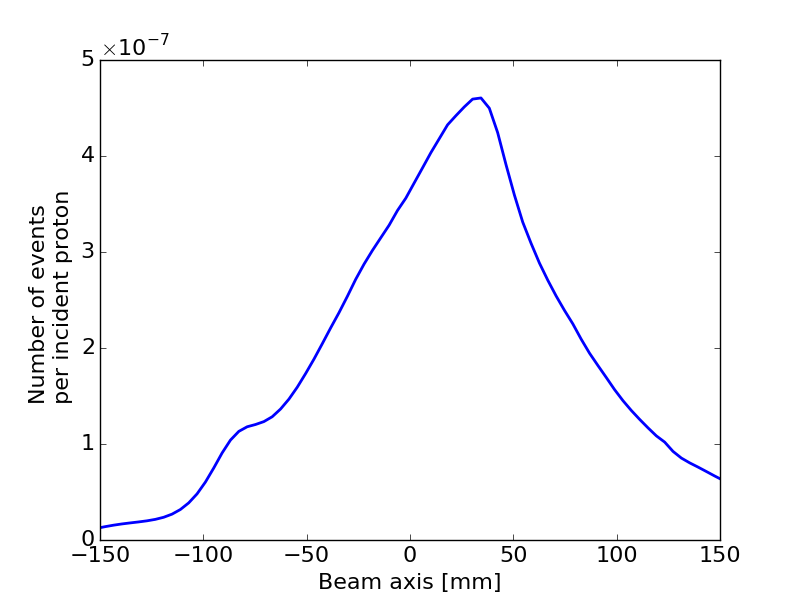
\includegraphics[width=0.48\textwidth]{./Figure/profileY_corr_r15.png}}\\
   \subfloat[\label{fig:fig_Results_Estimation_Camera_Profil_highStat_CC_simulation_Hadronth_MLEM}]{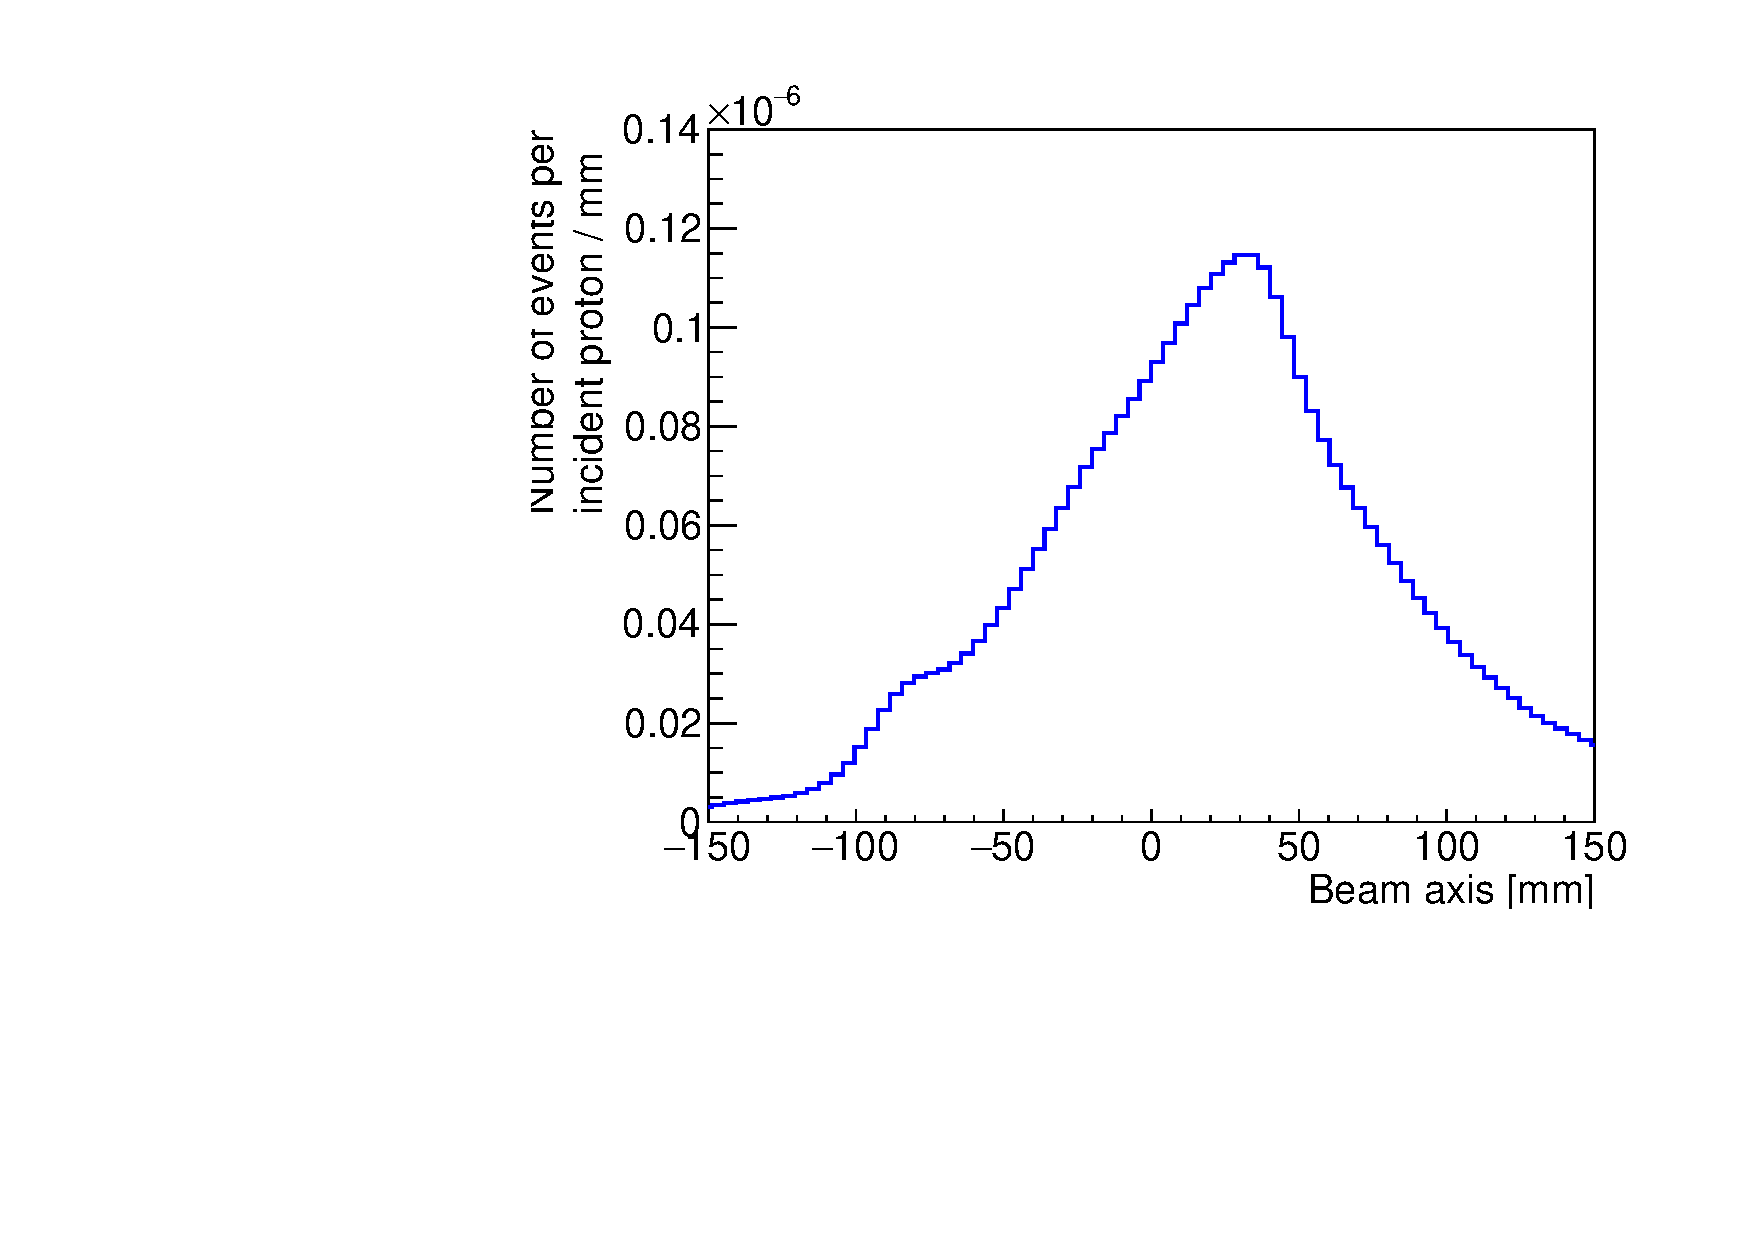
\includegraphics[width=0.48\textwidth]{03_GraphicFiles/chapter3/HT/new/reconstructed_histStat_profile_norm.pdf}}\\
  % \subfloat[\label{fig:fig_Estimation_Camera_CC_NURBS_Poisson_LC}]{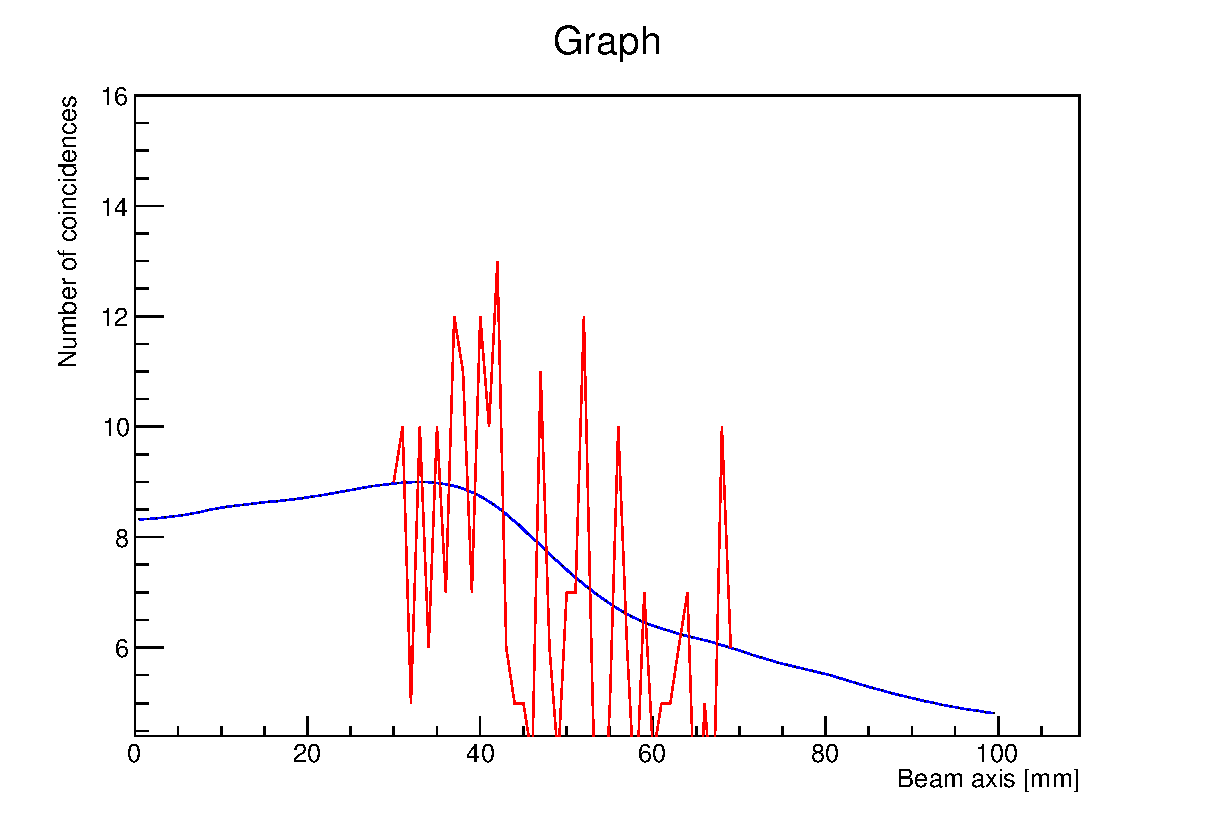
\includegraphics[width=0.33\textwidth]{./Figure/2017-08-02_Poisson_Nurbs_1e8_Article_LC.eps}}
  \subfloat[\label{fig:fig_Estimation_Camera_CC_NURBS_Poisson_LC}]{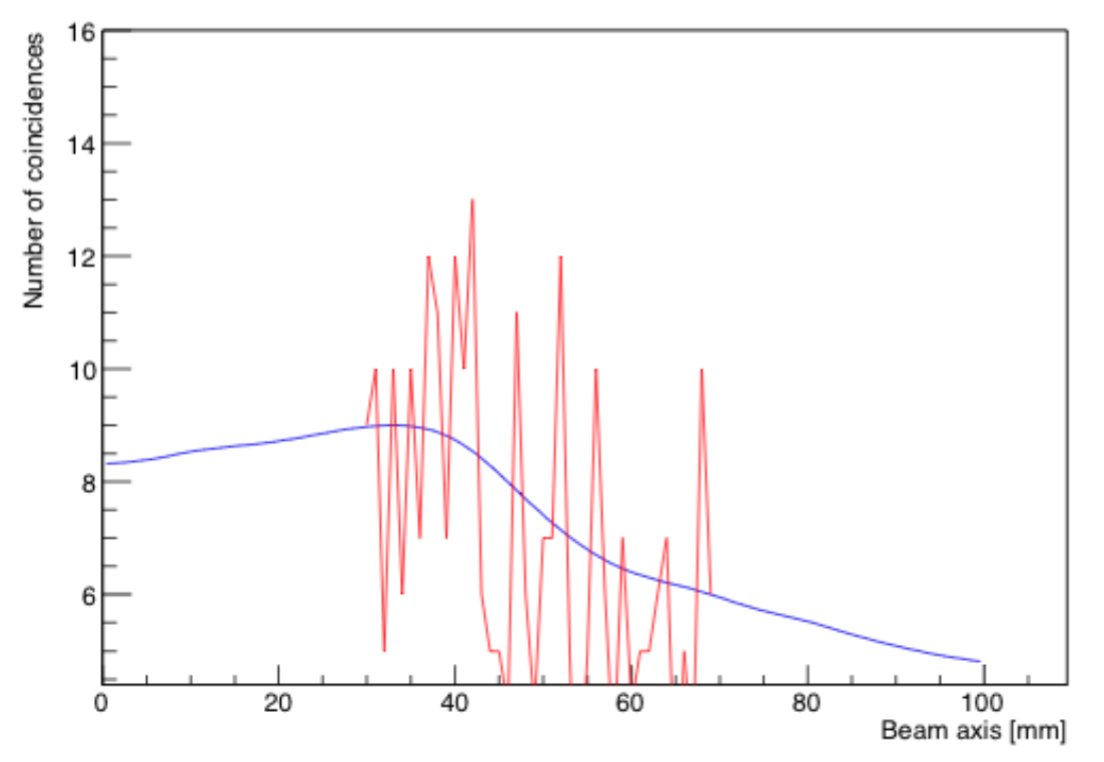
\includegraphics[width=0.48\textwidth]{./Figure/line_cone_NURBS.png}}
  % \subfloat[\label{fig:fig_Estimation_Camera_CC_NURBS_Poisson_MLEM}]{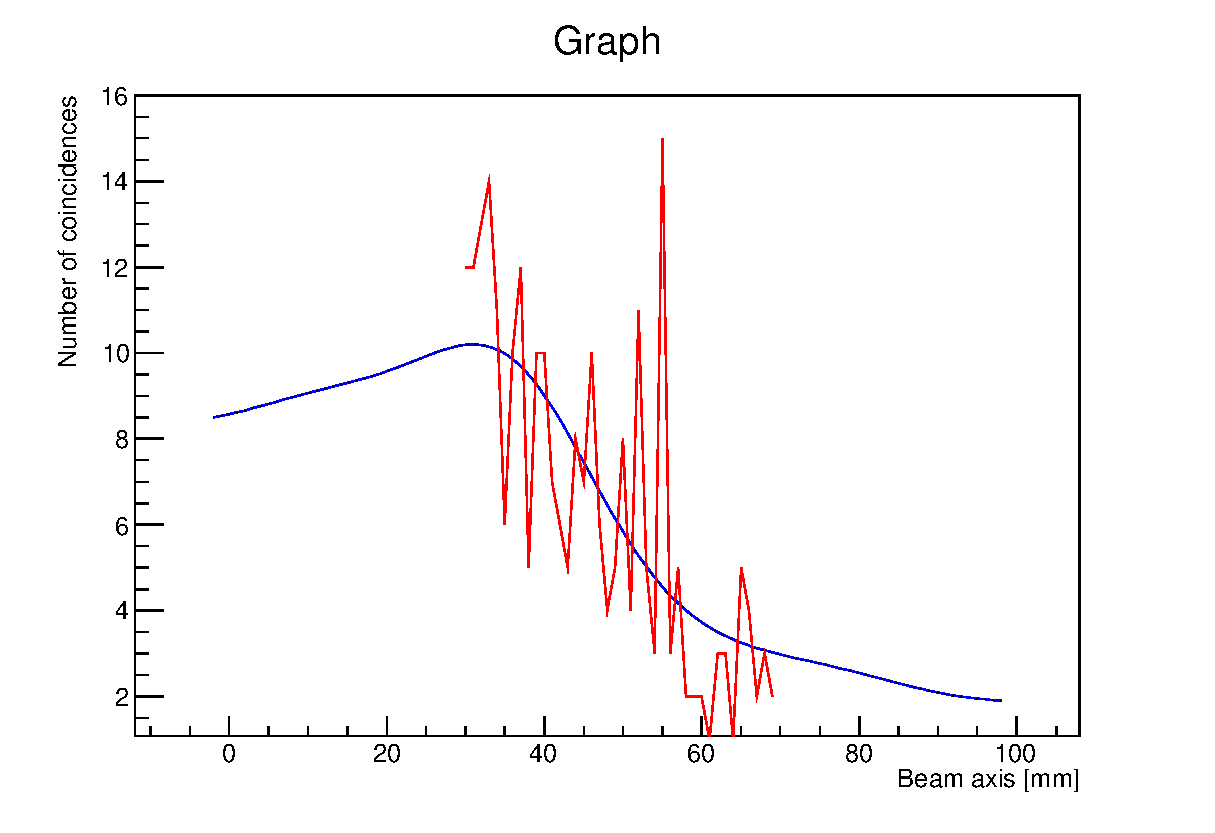
\includegraphics[width=0.33\textwidth]{./Figure/2017-08-02_Nurbs_Poisson_1e8_Article_MLEM.eps}}\\
  \subfloat[\label{fig:fig_Estimation_Camera_CC_NURBS_Poisson_MLEM}]{\includegraphics[width=0.48\textwidth]{03_GraphicFiles/chapter3/HT/MLEM_NURBS.png}}\\
  \caption{Data processing comparison for the same proton simulation with the line cone algorithm (left column) and the LM-MLEM algorithm (right column). The first row gives the reconstructed profile for $10^{10}$ incident protons. The second row shows the reference curve (blue) and the curve obtained with a $10^8$ incident protons subset.}% at the same statistics of $10^8$ incident protons.}
\end{figure}

\begin{figure}
  \centering
  % \subfloat[\label{fig:fig_Results_Chi2_Distribution_Variation_CC_simulation_Hadronth_LC}]{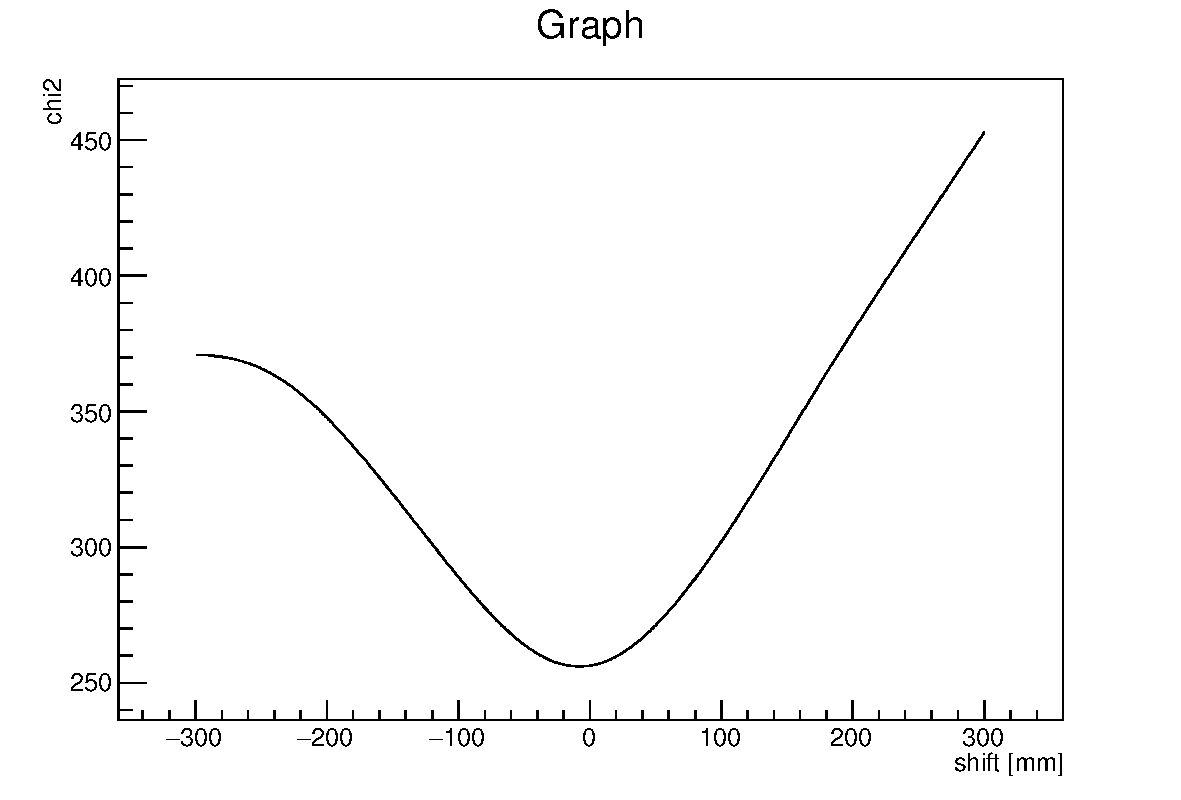
\includegraphics[width=0.33\textwidth]{./Figure/2017-08-02_Distribution_Chi2_1e8_LC.pdf}}
  \subfloat[\label{fig:fig_Results_Chi2_Distribution_Variation_CC_simulation_Hadronth_LC}]{\includegraphics[width=0.48\textwidth]{03_GraphicFiles/chapter3/HT/chi2_linecone.png}}
  % \subfloat[\label{fig:fig_Results_Chi2_Distribution_Variation_CC_simulation_Hadronth_MLEM}]{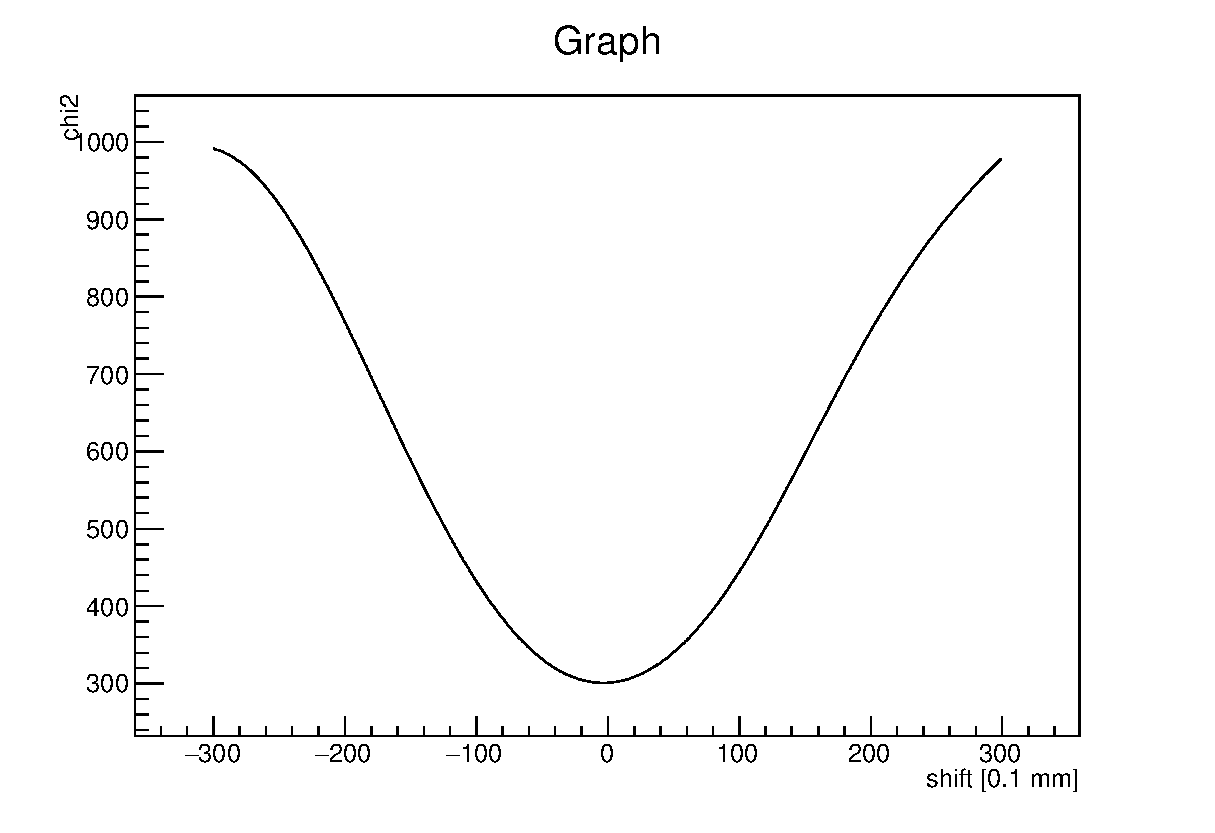
\includegraphics[width=0.33\textwidth]{./Figure/2017-08-02_Distribution_Chi2_Results_binning_1mm_ShiftNurbs0_1mm_1e8_article_MLEM.eps}}\\
  \subfloat[\label{fig:fig_Results_Chi2_Distribution_Variation_CC_simulation_Hadronth_MLEM}]{\includegraphics[width=0.48\textwidth]{03_GraphicFiles/chapter3/HT/chi2_MLEM.png}}\\
  % \subfloat[\label{fig:fig_Results_Precision_Distribution_Variation_CC_simulation_Hadronth_LC} ]{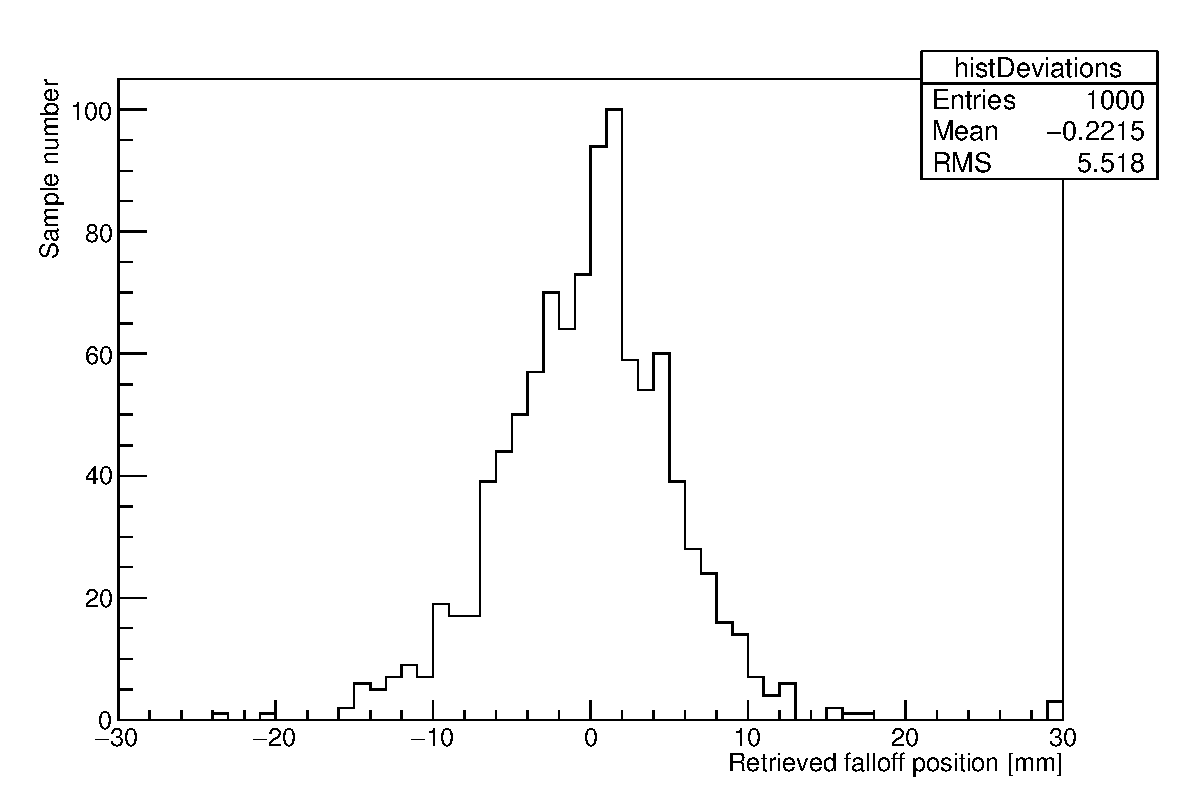
\includegraphics[width=0.33\textwidth]{./Figure/2017-08-02_Distribution_finale_1e8_Article_LC.pdf}}
  \subfloat[\label{fig:fig_Results_Precision_Distribution_Variation_CC_simulation_Hadronth_LC} ]{\includegraphics[width=0.48\textwidth]{03_GraphicFiles/chapter3/HT/deviation_linecone.png}}
  % \subfloat[\label{fig:fig_Results_Precision_Distribution_Variation_CC_simulation_Hadronth_MLEM} ]{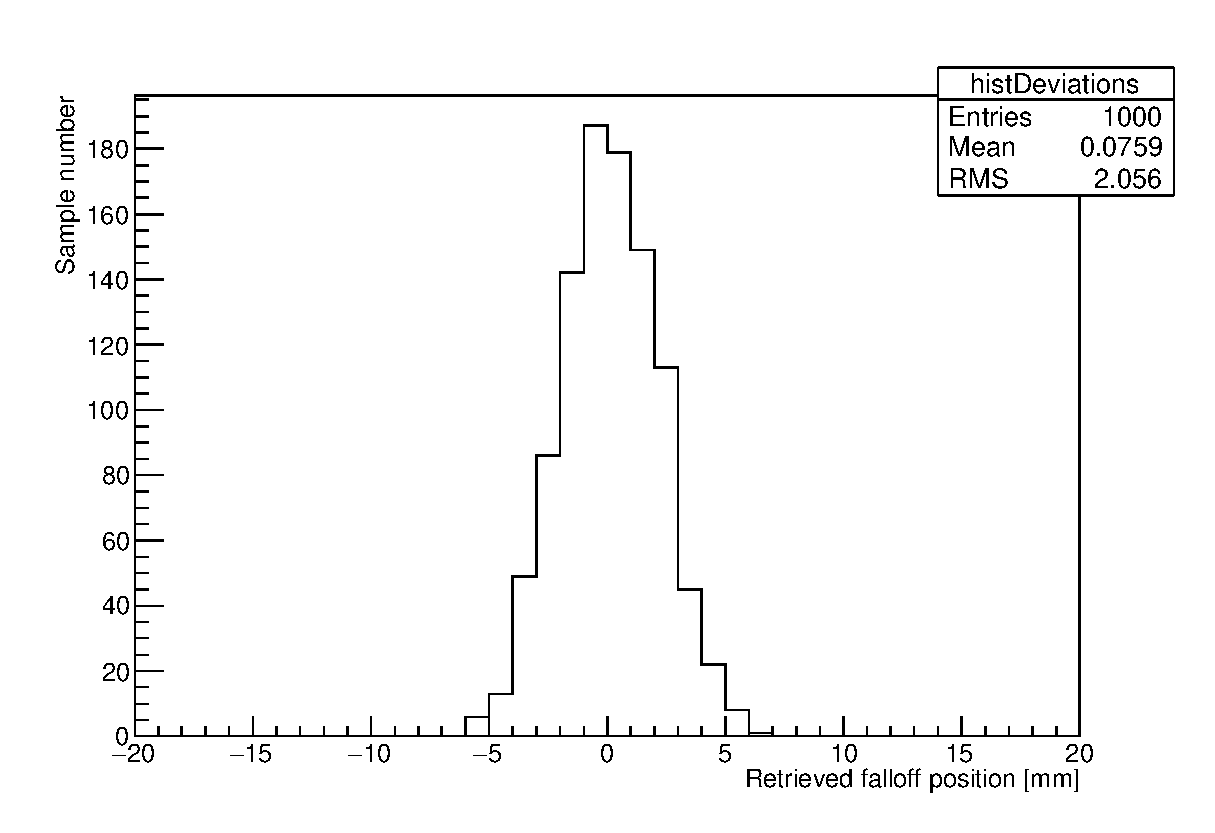
\includegraphics[width=0.33\textwidth]{./Figure/2017-08-02_FallOff_Results_binning_1mm_ShiftNurbs0_1mm_1e8_Article_MLEM.eps}}
  \subfloat[\label{fig:fig_Results_Precision_Distribution_Variation_CC_simulation_Hadronth_MLEM} ]{\includegraphics[width=0.48\textwidth]{03_GraphicFiles/chapter3/HT/deviation_MLEM.png}}
  \caption{Data processing comparison for the same proton simulation with the line cone algorithm (left column) and the LM-MLEM algorithm (right column). The first row shows the $\chi^2$ distribution for one data subset. The last row represents the distribution of the minimal calculated shifts for 1000 such subsets.}% at the same statistics of $10^8$ incident protons.}
\end{figure}

\begin{figure}
\centering
\subfloat[]{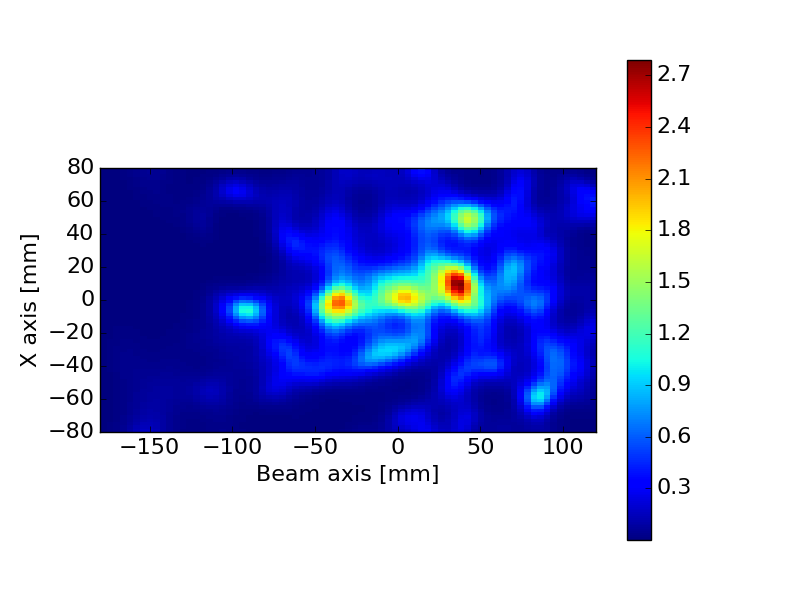
\includegraphics[width=0.5\textwidth,clip=true,trim=0 70 130 90]{03_GraphicFiles/chapter3/HT/projection2D_Z_corr_r20.png}}
%\subfloat[]{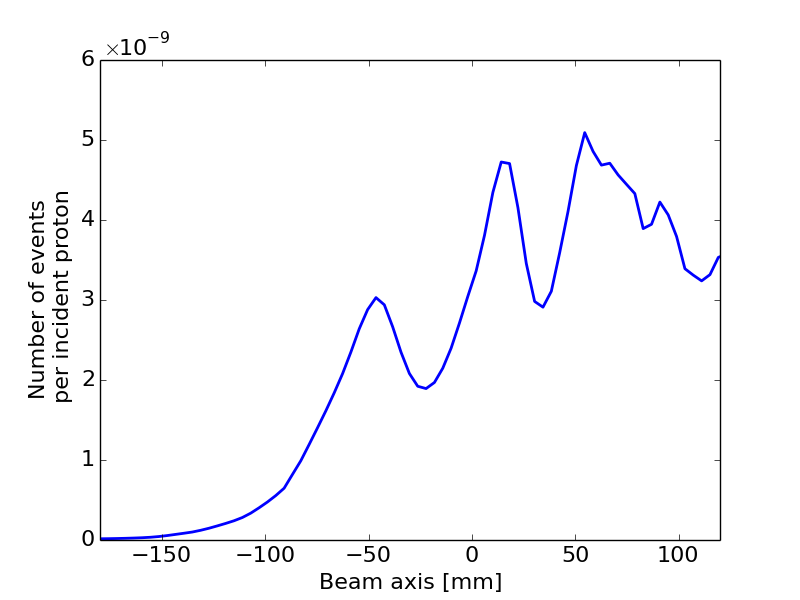
\includegraphics[width=0.5\textwidth]{./Figure/profileY_corr_r20.png}}\\
\subfloat[]{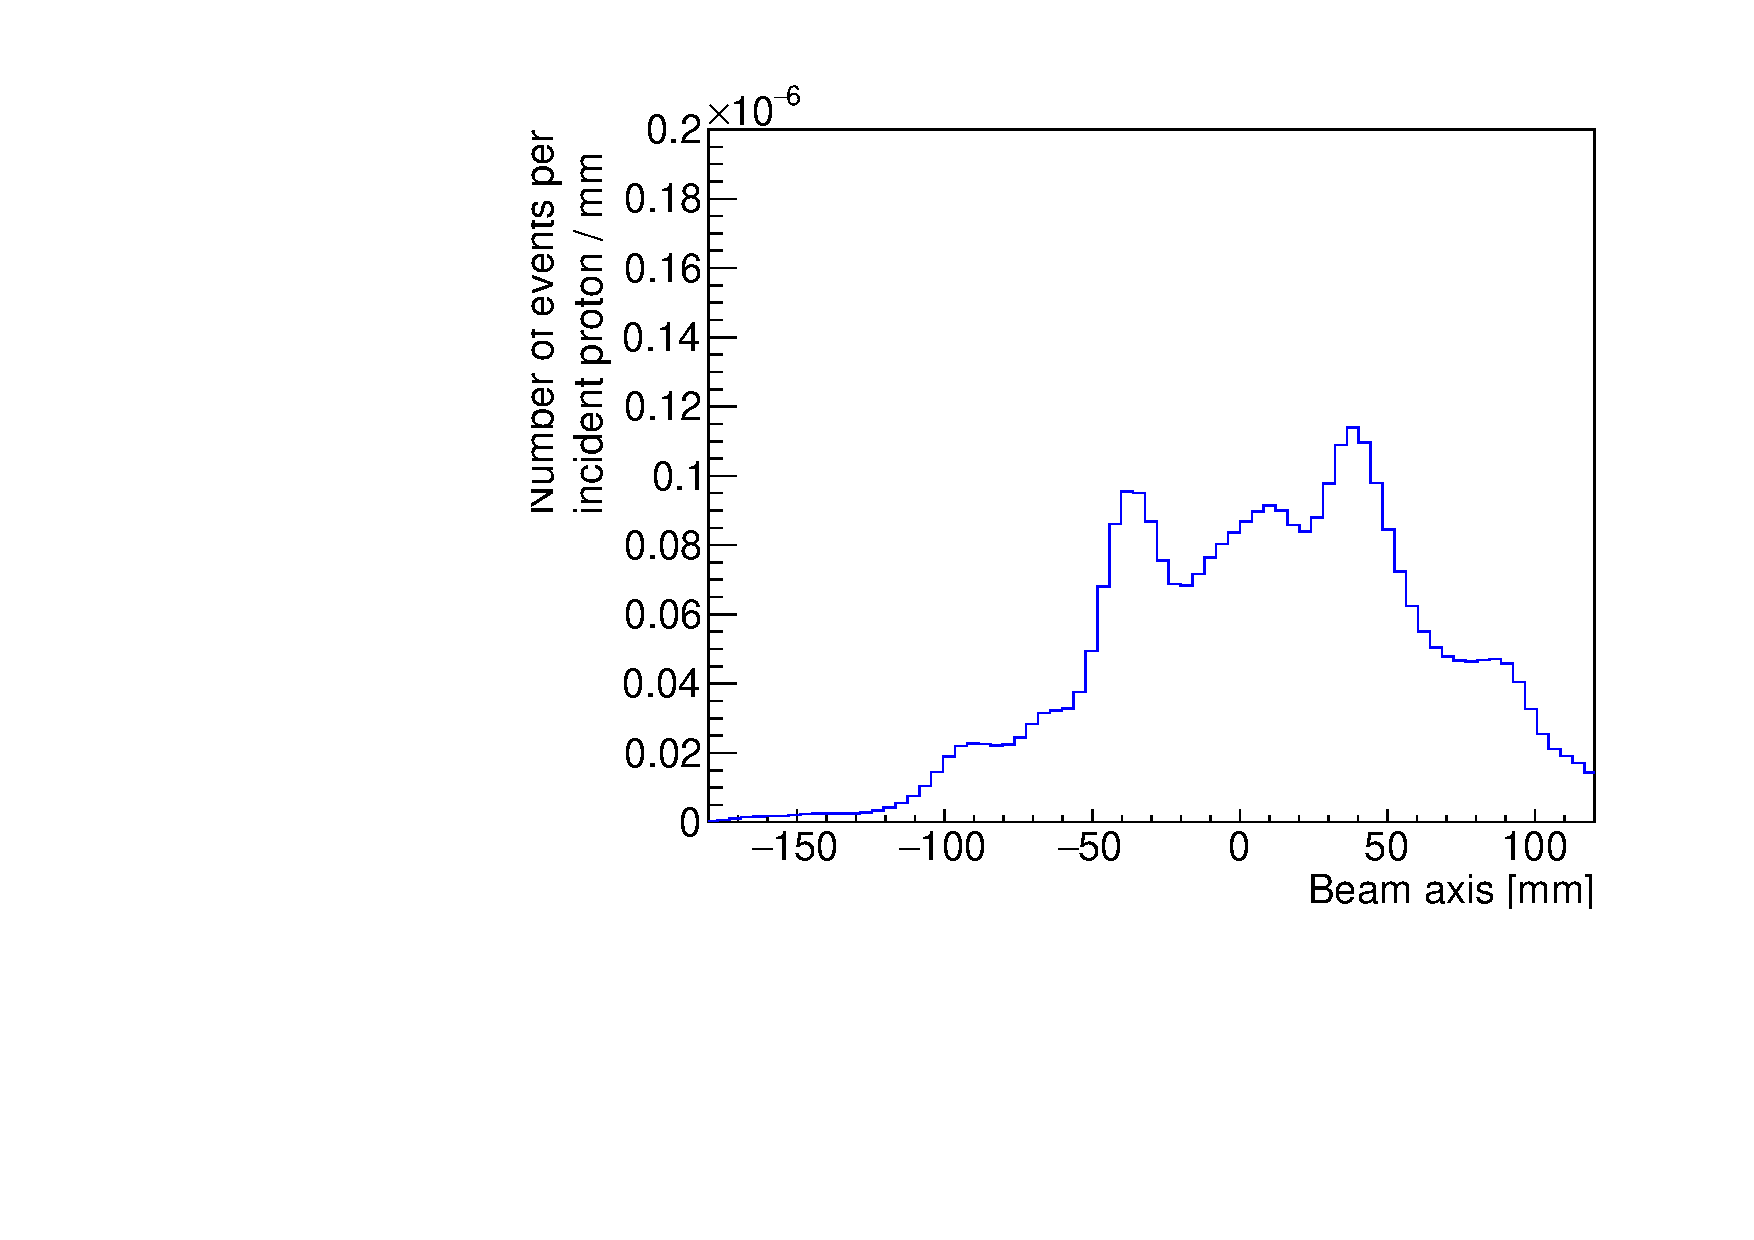
\includegraphics[width=0.5\textwidth]{03_GraphicFiles/chapter3/HT/new/reconstructed_lowStat_profile_norm.pdf}}\\
%\subfloat[]{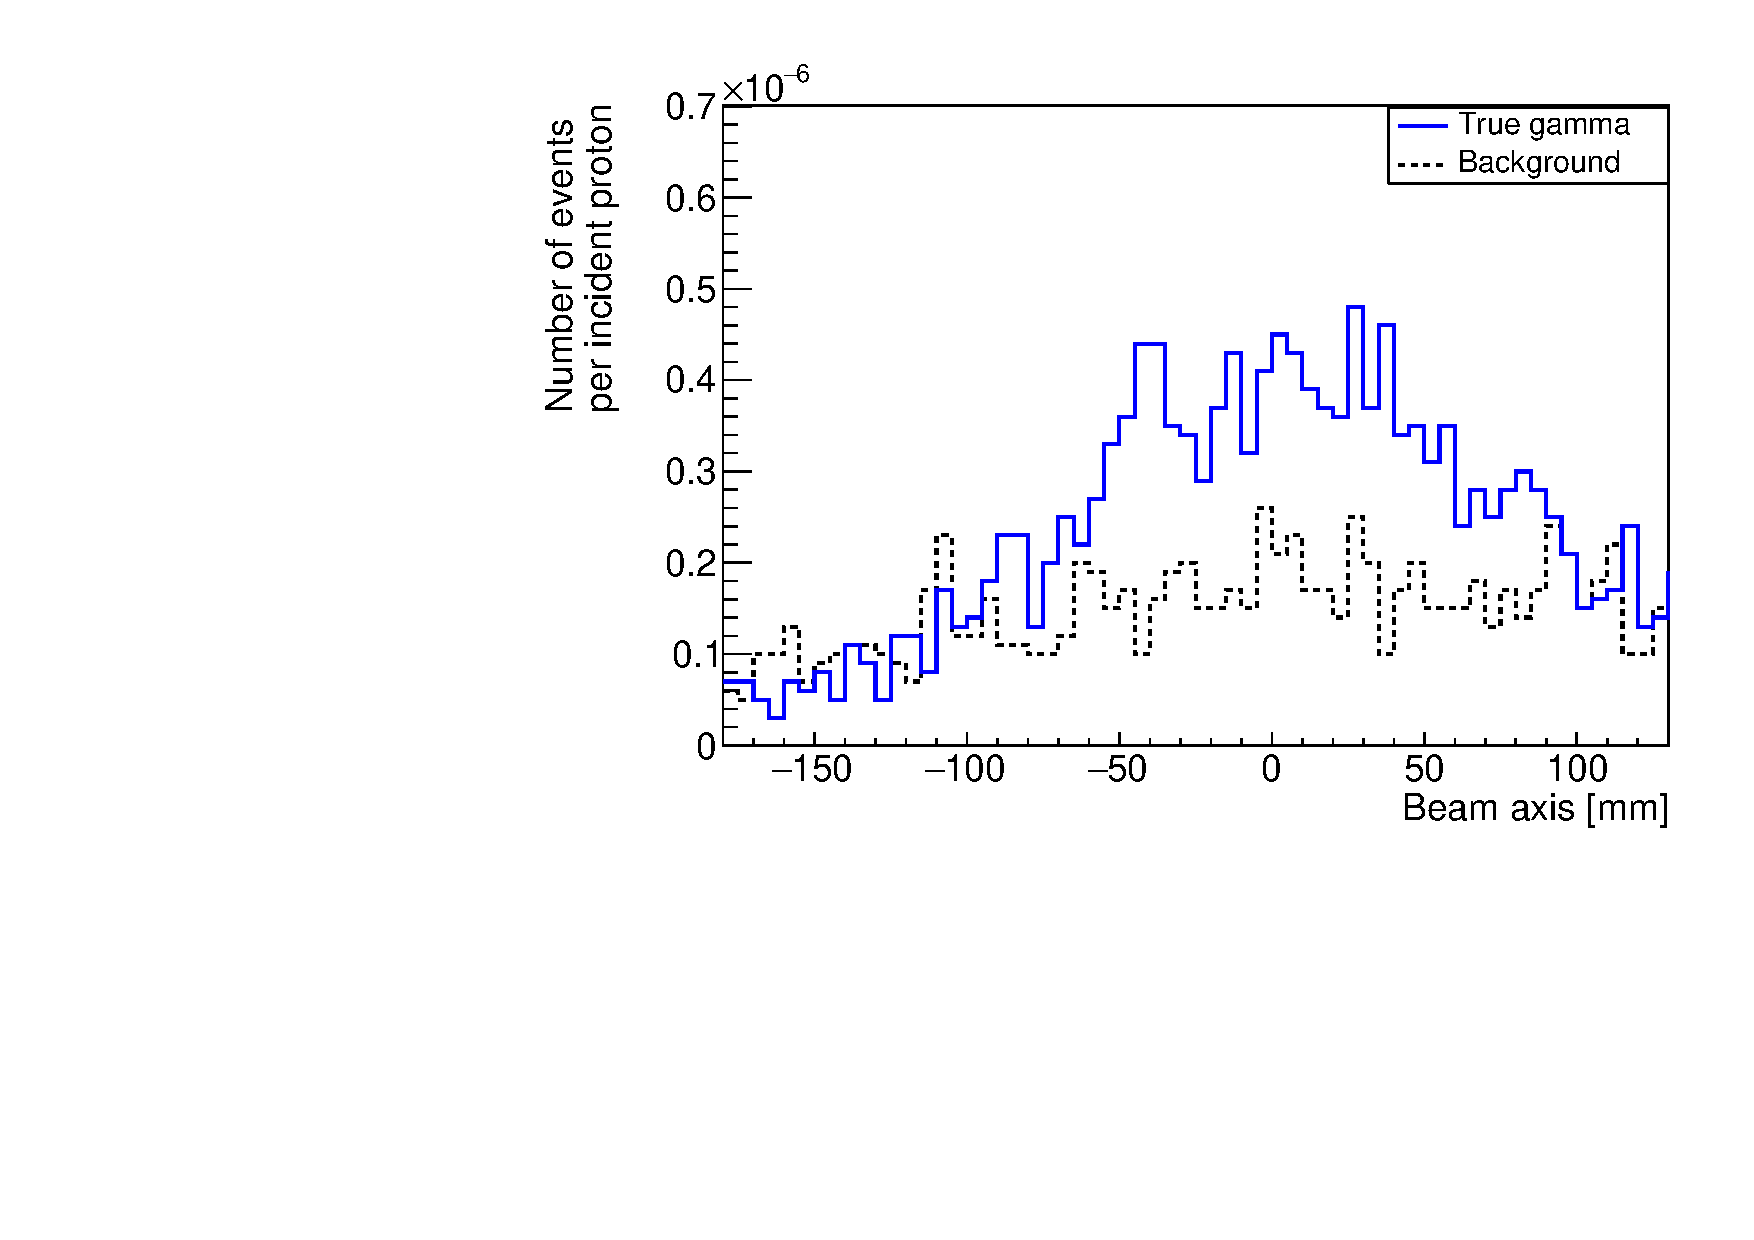
\includegraphics[width=0.5\textwidth]{./Figure/2015_02_16_Reconstruction_coinc_160MeVProton_TOF_6ns_file0to100_zoom.pdf}}
\subfloat[]{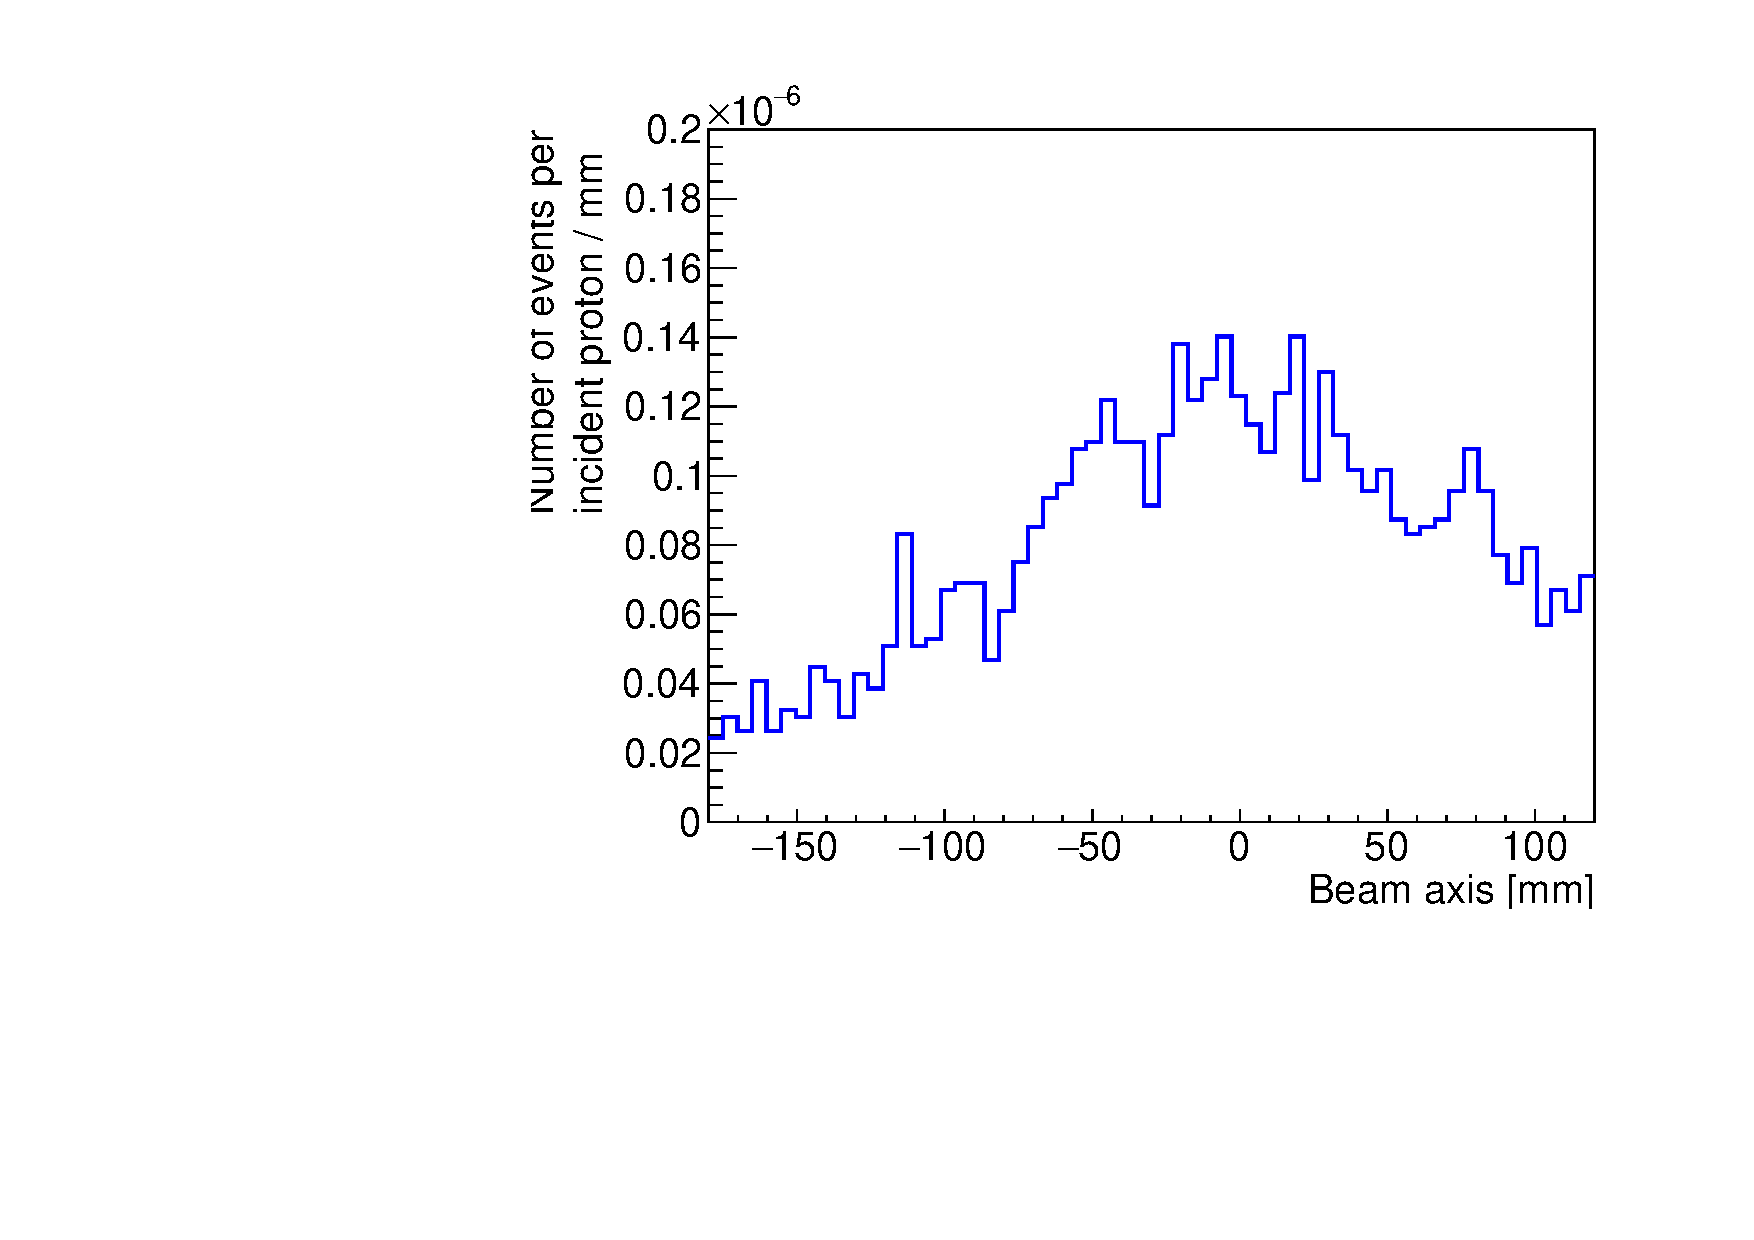
\includegraphics[width=0.5\textwidth]{03_GraphicFiles/chapter3/HT/new/recon_profile_line-cone_lowStat_norm.pdf}}

\caption{Line-cone and LM-MLEM reconstruction for a 160~MeV proton beam, $10^{8}$ total incident protons. The beam intensity is 1 proton per bunch. The Compton camera is centered at the expected Bragg peak position, $y=+50\,$mm. The time-of-flight event selection is applied on the collected data set. 20 iterations are performed for the MLEM reconstruction.
Figure (a) represents the MLEM reconstructed 2D image in the plane $(x,y)$, parallel to the camera entrance surface. The position $x=0\,$mm corresponds to the center of the PMMA phantom and the $y$ direction corresponds to the beam axis, with the target entrance at $y=-100\,$mm and the target end at $y=+100\,$mm.  In figure (b) the 1D profile along the $y$ axis is sketched. The profile fall-off is located at $y=+50\,$mm. Figure (c) shows the profile obtained by means of the line-cone algorithm for the same time-of-flight selected data.}
\label{fig:comparison}
\end{figure}


The analysis method described in section~\ref{MatMeth:precision} is applied to the different PG obtained profiles to retrieve the camera precision in the falloff identification. The results are shown in figure~\ref{fig:precision}, where the two reconstruction methods are represented by different markers.

\begin{figure}	
\centering
\includegraphics[width=0.7\textwidth]{03_GraphicFiles/chapter3/HT/2017-10-21_Precision_Comparaison_linecone_MLEM_Article_Fit.eps}
\caption{Fall-off retrieval precision (FRP) for two different reconstruction algorithms: line-cone and LM-MLEM. The precision is shown as a function of the total number of incident protons, in the range $1\times10^{8}$ to $5\times10^{9}$.}	
\label{fig:precision}
\end{figure}

The iterative MLEM reconstruction method enables one to achieve a better precision, with a reduction of about 3~mm of the falloff retrieval accuracy in the whole range of statistics explored. A linear behavior, highlighted by the performed linear fit of the two data sets, is verified with increasing number of primary protons, starting from the single spot scale of about 10$^8$ primaries, till $5\times10^9$ protons, which can correspond to the monitoring of a group of spot with the same planned range. 

\section{Discussion}

We studied in this simulation work the performance of the CLaRyS Compton camera prototype and its possible implementation as prompt gamma detector for ion beam therapy monitoring. The proposed analysis is focused on three main points: absolute gamma detection efficiency, true and random coincidence rate and camera precision in the identification of the prompt gamma emission profile fall-off.

The absolute gamma detection efficiency has been measured with the detector exposed to gamma sources at six different energies, and the efficiency variation as a function of the source position has been reported. The whole study has been performed with a fixed camera geometry, but different geometrical configuration can change the obtained results. In~\cite{Fontana_APPB} we tested the same prototype with two absorber configurations, showing an absolute efficiency reduction of a factor approximately two when reducing the absorber from a $8\times6$ block matrix to a $3\times3$ one. To this efficiency reduction corresponds an increased spatial resolution, probably given by the selection of gamma scattered with small angles. This hypothesis is confirmed by the efficiency variation generated by the applied energy thresholds. Indeed, for low energies, below 2~MeV, the increased efficiency in the central section of the camera active surface shown in figure~\ref{fig::efficiency_study}(a) is linked to the increased relative number of photons approaching the camera with small angles. These photons are more likely undergoing Compton scattering with a reduced energy deposition, which is recorded by an ideal detector and rejected by the energy threshold. The effect is all the more important as the primary gamma energy is limited, creating the peculiar energy dependence of the efficiency reduction observed in the results in figure~\ref{fig::efficiency_study}(b). Therefore, in case the compactness of the detector must be privileged, the efficiency reduction is not dramatic for the Bragg peak monitoring purpose. Moreover, such a compact configuration allows for the implementation of several detector heads, which can be set at different angles and provide additional spatial information. In case the highest possible efficiency is required, the distance between scatterer and absorber can be modified, knowing that for reduced distances the efficiency is increased because a minimal amount of scattered photons escapes the absorber field of view. On the other hand, a reduction of the inter-detector distance is not recommended for accurate TOF measurements (for fixed target-scatterer distance), given the uncertainty added by the detectors time resolutions. In addition to this, also the spatial resolution is affected by a reduction of the scatterer-absorber distance, given the increased amount of photons scattered with large Compton angles included in the collected events. Indeed, large angle scatterings tend to degrade the spatial resolution.   
Regarding the dependence of the efficiency on the Compton camera position, an accurate setup with respect to the expected Bragg peak position appears mandatory for the detection optimization.

A further study showed how this effect is mainly due to the cut applied on the scatterer detector. 
%The results emerged from the analysis of the rate of true and random coincidences with respect to the beam intensity show how at a realistic clinical intensity the signal-over-noise ratio is very low (less than 0.1) for both raw and reconstructed events and for proton and carbon beams. 
The study of the signal to noise ratio as a function of beam intensity was performed (see figure \ref{fig:coincidences}). The results show that, at clinical intensities, this ratio is very low. The TOF selection is effective in the case of carbon beams, where a significant proton and neutron contamination is expected. If we consider the case of proton beams, the amount of random and true coincidences is comparable at an intensity of about 1 proton per bunch, so that a clinical intensity reduction should be necessary to fit this configuration. Even if a possible image reconstruction is not excluded by the low signal-over-noise ratio detected at realistic beam intensity, given the fact that the random coincidence are distributed in an homogeneous way in the reconstructed volume, an intensity reduction can be an option in order to obtain more significant data sets. It must be noticed that the need for Bragg peak position online check is all the more necessary for distal spots, which are in general the first to be treated, so that a beam intensity reduction at the beginning of the treatment can be foreseen in case an accurate monitoring is strictly needed. This would not affect the treatment delivery, nor the planned patient rate in the clinical work-flow. 
In the case of carbon ions, the larger amount of secondary neutron produced during the patient treatment seems to require other background rejection methods in order to lead to an advantageous signal-over-background ratio. Note also that online filtering strategies  may be used to improve the quality of the date: already in figure \ref{fig:coincidences}, one can notice that the amount of reconstructed events is about half that of true gamma, which means that partial absorption in the absorber leads to events which cannot be reconstructed via the line-cone method. More refined pre-analysis could be used and have been proposed in \cite{Draeger:2017aa}.

The camera precision has been estimated starting from a reference prompt gamma emission profile obtained at high primary particle statistics ($10^{10}$), with the random extraction of 1000 data subsets per intensity and applying a minimization robust algorithm to define the shift of the identified profile fall-off with respect to the reference one.
The camera precision in the falloff identification rapidly increases for increasing primary particle statistics. A sufficiently good precision is achieved on a spot basis for proton beams, where the precision is about 2~mm with a MLEM reconstruction: a qualitative monitoring of each spot seems then possible. In order to achieve millimeter or sub-millimeter precision, some spot grouping methods must be considered. As a general result, the LM-MLEM iterative algorithm, which is now the standard for this kind of image reconstruction,  guarantees a better fall-off identification precision over the whole explored intensity range. However, MLEM does not exploit the additional information provided by the knowledge of the beam position in the transverse plane. In future studies, such a priori information should be considered in order to improve the reconstruction rapidity and image quality. At present, given the long calculation time required by the iterative algorithm, the line-cone reconstruction method can still be an option for on-line treatment check, when safety limit can be fixed in order to exclude severe deviation from the treatment planning and an interruption of the dose delivery in real time can be foreseen. Moreover, the TOF information can be included in the line-cone reconstruction method in order to constrain the emission on a single point, and improve its accuracy.

The Compton detection principle has already proven its potential in detecting prompt gammas for ion beam therapy monitoring purpose, and the CLaRyS Compton camera prototype shows promising results for this application. The detector is now at the final development stage, its components are being tested on beam in clinical facilities and a first beam test with a complete system is foreseen for the next year. New simulation studies are to ba carried out to benchmark the Compton camera device to other detection systems, like PET machines or collimated detectors, already used or tested in clinics for ion beam therapy monitoring.            



\clearpage
%\printbibliography[heading=subbibintoc]
